% !TeX encoding = UTF-8
\documentclass[twoside,english,1p,final,sort&compress]{elsarticle}
\usepackage[T1]{fontenc}
\usepackage[utf8]{inputenc}
\pagestyle{headings}
\usepackage{amsthm}
\usepackage{gensymb}
\usepackage{xspace}
\usepackage{amsmath}
\usepackage{accents}
\usepackage{multirow}
\usepackage{arydshln}
\usepackage{xcolor}
\usepackage{amssymb}
\usepackage{subcaption}
\usepackage{adjustbox}
\usepackage{placeins}
\usepackage[colorlinks = true]{hyperref}

% To have Times only in text not maths
\renewcommand{\rmdefault}{ptm}

\makeatletter

\theoremstyle{plain}
\newtheorem{thm}{\protect\theoremname}

% specify here the journal
\journal{International Journal of Mechanical Sciences}

% use this if you need line numbers
\usepackage{lineno}

\makeatother

\usepackage{babel}
\providecommand{\theoremname}{Theorem}

%\newcommand{\w}{\mbox{\large\ensuremath{\mathsf{w}}}}
%\newcommand{\A}{\mbox{\large\ensuremath{\mathsf{A}}}}
%\newcommand{\B}{\mbox{\large\ensuremath{\mathsf{B}}}}
%\newcommand{\C}{\mbox{\large\ensuremath{\mathsf{C}}}}
\newcommand{\dotp}{\boldsymbol{\cdot}}
%\newcommand{\ccirc}{\kern0.5ex\vcenter{\hbox{$\scriptstyle\circ$}}\kern0.5ex}
\newcommand{\e}[1]{\exp\left({#1}\right)}
\newcommand{\lay}[1]{^{(#1)}}
\newcommand{\mdot}[1]{\accentset{\mbox{\bfseries .}}{#1}}
\newcommand*{\ie}{\emph{i.e.}\@\xspace}
\newcommand*{\versus}{\emph{vs.}\@\xspace}
\newcommand*{\eal}{et \emph{al.}\@\xspace}
\newcommand*{\eg}{e.g.,\@\xspace}
%\newcommand{\ERMS}{\text{E}_\text{RMS}}
\newcommand{\AARE}{\text{E}_\text{AAR}}
\newcommand{\R}{\text{R}}
%\newcommand{\Dev}	{\mbox{\Large\ensuremath{\mathsf{s}}}}
%\DeclareMathOperator{\sech}{sech}
%\DeclareMathOperator{\sigmoid}{sig}

\usepackage{esvect}
% Redefine the esvector shape to remove overlapping
\def\traitfill@#1#2#3#4{%
  $\m@th\mkern2mu\relax#4#1\mkern-1.5mu %on met \relbaredd au d\'ebut
   \cleaders\hbox{$#4\mkern-0.3mu#2\mkern-0.3mu$}\hfill %remplit avec relbareda
   \mkern-1.5mu#3$%
}
\renewcommand{\overrightarrow}{\vv}

\begin{document}
\begin{frontmatter}

\title{Phenomelogical and artificial neural network models' comparison study for hot deformation of AISI P20: Interpolation and extrapolation predictions}

\author[LGP]{Pierre Tize Mha}
\author[LGP]{Amèvi Tongne}
\author[LGP]{Olivier Pantalé \corref{cor1}}
\ead{Olivier.Pantale@enit.fr}
\ead[url]{http://www.enit.fr}

\cortext[cor1]{Corresponding author}

\address[LGP]{Laboratoire Génie de Production, INP/ENIT, Université de Toulouse, 47 Av d'Azereix, Tarbes, France 65016}

\begin{abstract}
Non-linear numerical modeling is increasingly used for the simulation of complex processes such as forming or machining. The constitutive laws necessary for these simulations are therefore becoming more and more complex regarding the increasingly precise consideration of physical phenomena (plasticity, thermal dependence, damage ...) and their implementation in numerical codes requires the identification of many parameters. The use of these constitutive laws for dynamic or quasi-static applications requires the identification of these parameters under conditions close to those encountered during the real process, mainly in terms of deformation, strain rates, and temperatures. The availability of a constitutive law in the finite element codes does not guarantee the success of a study to be carried out if it does not comply with the model development criteria. This is because the models integrated in the numerical codes are not developed based on forms that are adjustable to any type of study. In this study, a new form of non-linear constitutive flow law based on the Modified Zerilli--Armstrong model, which can answer the above problem, has been developed to apply it to the numerical simulation of two different tests (a quasi-static compression test, the necking of a circular bar). This flow law is based on the modified Zerilli--Armstrong model, which, together with the new modified Johnson--Cook model, has been compared to appreciate the relevance of the proposal. For that, an implementation of this new law via the VUHARD subroutine into the Abaqus/Explicit finite element code was made to model the two tests. The comparison of the results obtained (from identification) by our proposed law with those obtained using the NMJC shows that this new law better approaches the experiments than the other one. This is also showed through the numerical results using the Abaqus software. It can be said that this way of formulating a flow law allows to highlight the great performance of the proposed approach. Although this law has been used only used for quasi-static tests, we can say that it can also be used in dynamic tests.
\end{abstract}

\begin{keyword}
Zerilli--Armstrong flow law \sep Constitutive Behavior \sep Finite Element Method \sep Numerical Implementation \sep Johnson--Cook flow law
\end{keyword}

\end{frontmatter}
\linenumbers

%--------------------------------------------------------------------------
\section{Introduction\label{sec:Introduction}}
%--------------------------------------------------------------------------
\textcolor{red}{Due to technological advances, industries are constantly looking for innovations to maintain their competitiveness. For the metallurgical industry, these innovations involve the development of new materials. In conjunction with the implementation of these new materials, it becomes necessary to characterize their thermomechanical behavior, in particular in order to feed the data bases used by the numerical simulation models more and more widespread nowadays \cite{Trimble-2020-Finite, Yuan-2021-Particle}}.

\textcolor{red}{Among the different approaches used, the finite element method (FEM) is one of the numerical methods that has become the most popular nowadays. Like any numerical method, the accuracy of the solution depends very strongly on the constitutive equation describing the behavior of the material and implemented in the computational code \cite{Li-2021-Finite, Liu-2021-Finite}. This constitutive equation is linked to the mathematical model that describes it. This choice is not entirely free, insofar as the choice of the behavior law (speaking of an analytically formulated model) used to describe the behavior of a material is guided by its availability in the finite element codes \cite{Miller-2021-Thermomechanical}. This forces an adaptation between the studied material (which is real) and the behavior law (representative mathematical model) available in the FEM code which is not necessarily the one able to describe the behavior of the studied material. The problem of the non flexibility of the models available in the finite element codes appears immediately and limits the adequacy of the model to the reality of the behavior since the behavior laws established and available in the FEM codes are for the most part specific to a particular material or class of materials. In other words, as soon as they are applied to materials different from the one for which they were originally developed, they find their limits because they do not manage to represent the reality described by the experiment as one would wish. It is therefore interesting to think about developing a method that can be applied to any material of any class and implemented in a finite element code. This approach involves a number of parameters depending on the material studied, but with a more global mathematical form adaptable to a wider range of materials. In this study, we propose an approach allowing a better adaptability of the behavior law to various materials. To justify the relevance of this proposal, let us first examine the models developed so far and try to see if some of them meet this need}.

\textcolor{red}{According to the literature, analytical models describing the behavior of materials can be grouped into three categories: empirical models, semi-empirical models, and physical models. Empirical models describe the behavior of the material by considering macroscopic quantities without considering its microstructure, whereas physical models consider the microstructure. As for the semi-empirical models, they try to be at the border between the empirical and physical models. Among a large number of models, the Johnson--Cook (JC) \cite{Johnson-1983-Constitutive, Johnson-1985-Fracture} and the Zerilli--Armstrong (ZA) \cite{Zerilli-1987-Dislocation} models are the best known and available in finite element codes. The JC model is widely used because it is simple to use and has fewer constants to be determined \cite{Khan-2004-Quasi-static, NematNasser-2003-Thermomechanical}. However, this model, in its original state, contains some problems related to the phenomena describing the behavior of the material. We refer here to strain hardening, strain rate hardening, and thermal effects that are described separately in the JC model as analyzed by Jia \eal \cite{Jia-2021-Modified-JC}. To overcome this difficulty, several modified forms of the Johnson--Cook model have been developed in the past \cite{Rule-1998-Revised-JC, Vural-2003-Large, Lin-2010-Modified-JC, Lin-2012-Phenomenological, Li-2013-Modified-JC, Zhou-2019-Research, Zhang-2015-Modified-JC}}.

\textcolor{red}{Due to its more physical formulation, the ZA model is preferred over the JC model because it allows for the coupling between strain rate and temperature effects \cite{Johnson-1988-Evaluation, Voyiadjis-2005-Microstructural, Dey-2007-Influence}. However, the drawbacks of this model are related to the temperature limit value of the test. Indeed, this model applies only to low strain rates and for temperatures limited to $0.6~T_m$ (where $T_m$ is the melting temperature of the material) \cite{Chiou-2005-Strain, Lee-2005-Strain, Chen-2007-Comparative, Lee-2006-Effects}. Moreover, this model, in its original form, does not take into account the coupling between deformation and temperature effects \cite{Samantaray-2009-Thermo-viscoplastic}. In order to reduce these shortcomings (\eg applying this model over a wider temperature range) of the ZA model, Modified Zerilli--Armstrong forms (MZA) have been proposed by several authors over the last past years \cite{Nemat-2004-Plasticity, Lennon-2004-Influence, Muralli-2017-Performance, Cheng-2021-Modified-ZA, Muralli-2021-Finite}}.

\textcolor{red}{These two approaches are among the most popular and the choice depends on the effectiveness of the method for a given problem. So we have on the one hand, the JC formulation and its variants and on the other hand the ZA approach with its variants too. Another approach proposed by Lin \eal \cite{Lin-2010-Modified-JC} is to combine the JC model with the MZA model (in its modified form proposed by Samantaray \eal \cite{Samantaray-2009-Thermo-viscoplastic}). This approach allows combining on the one hand the factor taking into account the strain hardening effects described by the JC model and on the other hand the factor describing the strain rate effects and the thermal softening described by the MZA model in a unified formulation. The major difficulty of all the variants mentioned above is the restriction of the parameters on which the model depends, thus limiting the applicability domain of the developed model. Therefore, it seems necessary to look for a method that does not limit the number of parameters, unlike the approaches mentioned above, and that can describe more accurately the reality observed by the experiment}.

\textcolor{red}{Artificial neural networks (ANNs) offer an alternative way to solve these problems. ANNs are currently used to solve problems that are difficult to conceptualize using traditional computational methods. Thus, unlike a classical approach based on a regression method, an artificial neural network does not need to know the mathematical form of the model it seeks to reproduce and can therefore learn directly from experimental data without any prior assumption on the nature of the input parameters and their interactions. Thus, artificial neural networks can enable new approaches for modeling material behavior and have been successfully applied for the prediction of constitutive relationships of some metals and alloys \cite{Lin-2008-ANN, Lu-2011-ANN, Ashtiani-2016-CSP, Huang-2021-CMM}. Although this approach is very effective, it does not allow the interpretation of the obtained results, because it does not take into account the physics of the phenomena for the considered material}.

\textcolor{red}{From the above, we can retain that there are two main families of models to describe the behavior of a material. On the one hand, analytical models presenting a problem of flexibility and on the other hand, implicit models, based on neural networks, more adaptable but presenting a problem of physical interpretation. It is therefore interesting to develop a physical model that is able to adapt to any material and can be efficiently implemented in a finite element code. In this perspective, we propose here a new formulation based on the MZA model, whose interest is to answer the two problems mentioned above. To appreciate the relevance of our approach, we used the Abaqus/Explicit software which offers the possibility to implement a new behavior law using a FORTRAN VUMAT or VUHARD subroutine following the example of the works proposed by \cite{Gao-2007-FRT, JansenVanRensburg-2012-TSV, Duc-Toan-2012-MJC, Ming-2018-ERV}}.

\textcolor{red}{The main paragraphs of this work are as follows: Section \ref{sec:ConstLaws} presents two  known constitutive laws which will serve as the basis of the the proposed one presented in Section \ref{sec:ProposedModel}. Since this model is new and will be used to perform a numerical model using Abaqus, the three derivatives of flow stress $\sigma$ with respect to the strain $\varepsilon^p$, the strain rate $\mdot{\varepsilon}^p$ and temperature are required. So, determination of these derivatives is done in this Section. Section \ref{sec:Application} is devoted to the comparison of the proposed model to the others one where identification is done on a 100Cr6 steel. Section \ref{sec:NumSimulations} details the numerical results of the models identified in Section \ref{sec:Application} using the cylindrical compression test and the necking of circular benchmark tests. Conclusion and future works are detailed in Section \ref{sec:Conclusion}}.

%----------------------------------------------
\section{Experimental procedure}
%----------------------------------------------
The material used in this study is the modified carbon alloy AISI P20 whose chemical composition is given in the Table. Cylindrical specimens were machined with an initial diameter of $10$ mm and a height of $15$ mm. Hot compression tests were conducted on a Gleeble-3800 thermo-simulator (Figure \ref{fig:Gleeble3800}), at temperatures of $1050^\circ$C,  $1050^\circ$C,  $1100^\circ$C,  $1150^\circ$C,  $1200^\circ$C and  $1250^\circ$C with strain rates of $0.001\ \text{s}^{-1}$, $0.01\ \text{s}^{-1}$, $0.1\ \text{s}^{-1}$, $1.0\ \text{s}^{-1}$, $2.0\ \text{s}^{-1}$ and $5.0\ \text{s}^{-1}$. Thin tantalum sheets were used as a lubricant material at the contact surface of anvils and specimen to minimize the frictions during hot deformation. The samples were heated to $1260^\circ$C temperature and were held for $5$ min to eliminate thermal gradients at the test temperatures. Then cooled to test temperature where the specimen is held $1$ minute before deformation. After compression the specimen is quencted rapidly for microstructure studies. The procedure of this test is illustrated in Figure \ref{fig:Heating}.
\begin{figure}[!ht]
\centering
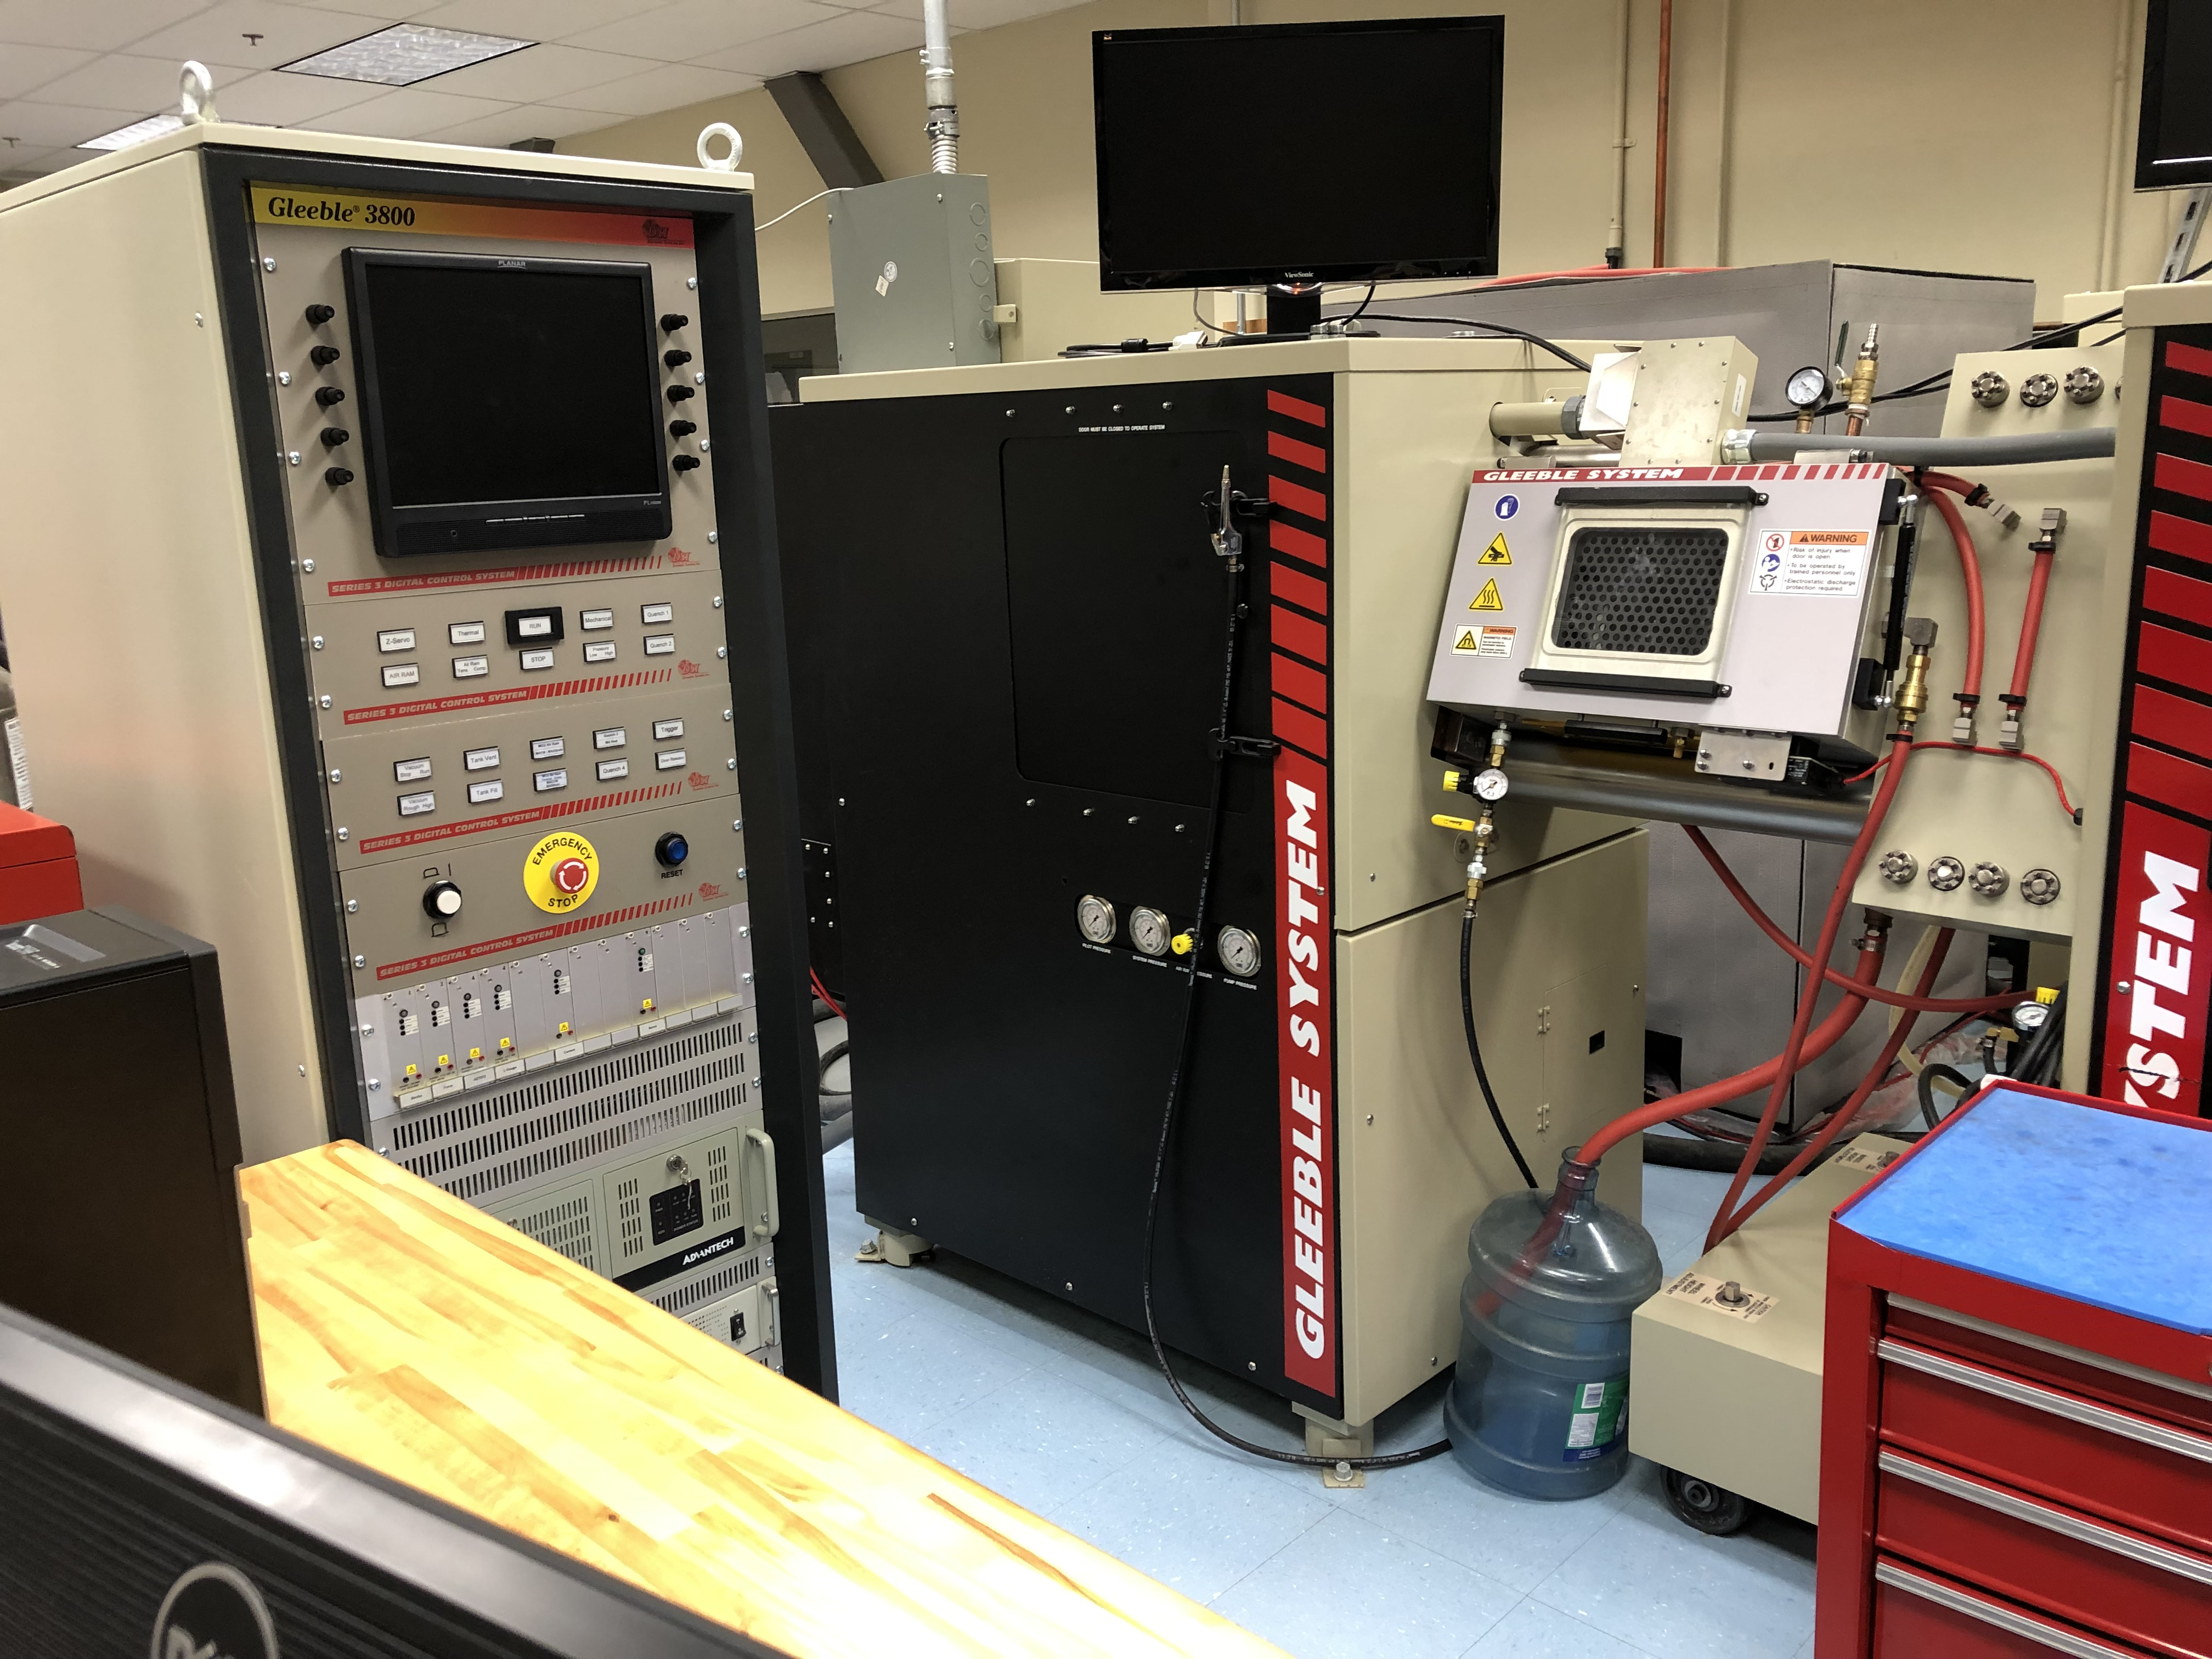
\includegraphics[width=0.9\columnwidth]
{newFigures/Gleeble-3}
\caption{Gleeble 3800 simulator system}
\label{fig:Gleeble3800}
\end{figure}
\begin{figure}[!ht]
\centering
\includegraphics[width=0.9\columnwidth]
{newFigures/GleebleDesign}
\caption{Schematic diagram of the experimental process.}
\label{fig:Heating}
\end{figure}
\begin{table}[h!]
\centering{}
\caption{Chemical Composition of the AISI P20 Steel (Weight Percent)}
\scalebox{0.9}{
\begin{tabular}{lcccccccc}
\hline
C  &Mn & Mo   & Si   & Ni       &Cr& Cu & Other& Balance\\
\hline
 0.30        &       0.89      &0.52		   &	0.34     &	 0.68          &1.86& 0.17& Microalloying& Iron\\
\hline
\label{tab: Composition}
\end{tabular}}
\end{table}
%------------------------------------------------------------------------
\section{Results and discussion\label{sec:ConstLaws}}
%------------------------------------------------------------------------

%------------------------------------------------------------------------
\subsection{Flow stress behaviour}
%------------------------------------------------------------------------
The flow stress curves obtained from the compression tests performed on Gleeble-3800 simulator for each test condition are shown in Figure \ref{fig:rawData}. From these curves it can be seen that the flow stress increases with increasing strain rate but decreases with increasing temperature. It should be noted that the strain influences the flow stress. Indeed, for all strain values below $0.2$, the stress increases with strain before reaching a peak value at low strain rates and then decreases to maintain a stable value until the end of the test. The peak stress value increases with strain rate but decreases with temperature. For higher strain rates ($1.0\ \text{s}^{-1}$, $2.0\ \text{s}^{-1}$ and $5.0\ \text{s}^{-1}$) the flow stress increases throughout the test. The slight increase in stress at low strain rates when the strain is large is due to friction between the specimen and the grip during the test. For low strain rates, lubrication is lost over time and therefore friction occurs. This results in a progressive increase in stress.

To explain the overall behaviour of the flow stresses observed during this test, we will rely on two fundamental phenomena that can be observed during a compression test: Dynamic Recovery (DRC) and Dynamic Recrystallization (DRX). At the beginning of the deformation, the amount of dislocations increases and they start to move, leading to a rapid increase in stress known as work-hardening. As the strain continues to increase, the dislocations are set in motion, leading to a stress relaxation phenomenon usually known as DRC. During this DRC mechanism, some of the dislocations are removed, due to their combination with another dislocation, or due to their integration into a grain boundary, and some of them are rearranged and formed as sub-grains within the initial grains. The combination of these dislocations moderates the increase of dislocations linked to strain hardening and thus controls the amount of energy stored in the material and manages the increase in flow stress. DRX consists of the germination of new grains, at the borders or inside the initial grains. These two phenomena therefore explain the different shapes of the flow stress curves observed for this alloy. As an example, the Figure \ref{fig:BarNecking} , and Figure \ref{fig:AfterCompM} show the microstrutures of AISI P20 before and after compression. As observed on the flow curves, it can be seen that recrystallisation is almost complete for this temperature and strain rate. Indeed, most of the grain boundaries start to form new grains. The identification of the behavioural laws of these curves will be done in the next section in order to predict its behaviour in any test condition. This will be done on the one hand to test the ability of the models to describe an interpolation and on the other hand to do extrapolation.
\begin{figure}[!ht]
\centering
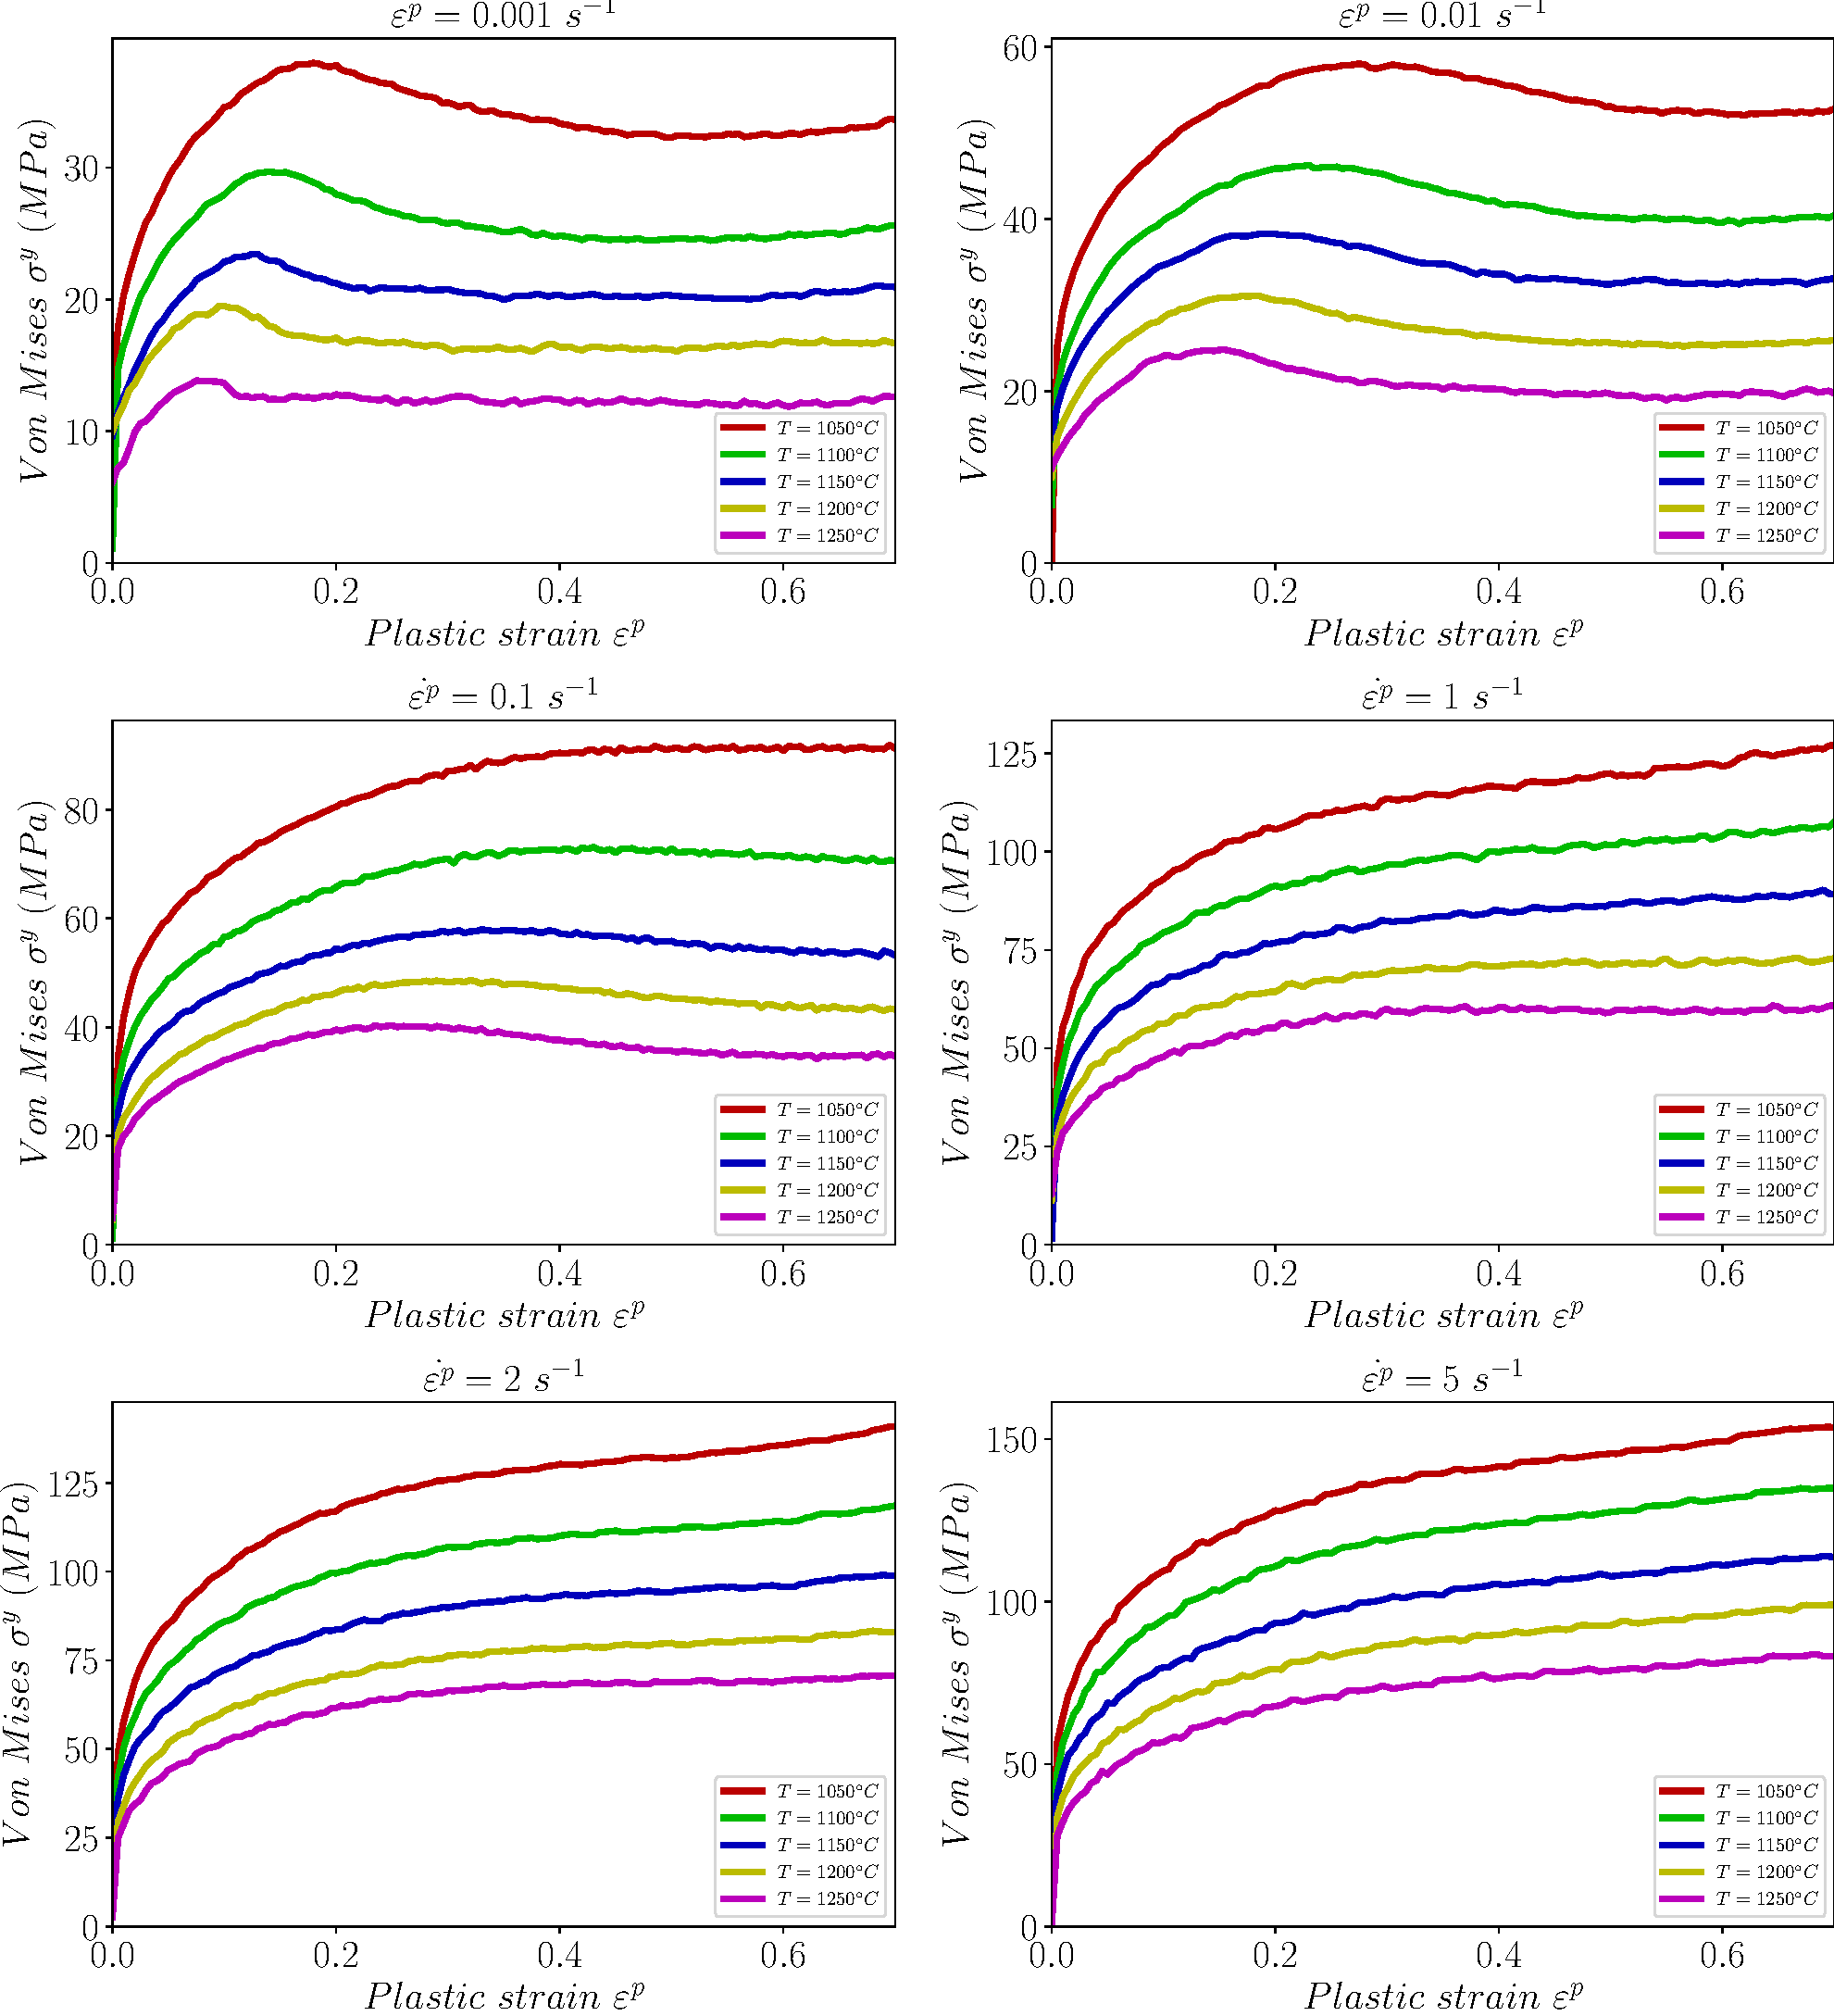
\includegraphics[width=1.02\columnwidth]
{newFigures/rawData}
\caption{Flow stress-strain curves of AISI P20 alloy at various temperatures and strain rates.}
\label{fig:rawData}
\end{figure}
\begin{figure}[!ht]
\centering
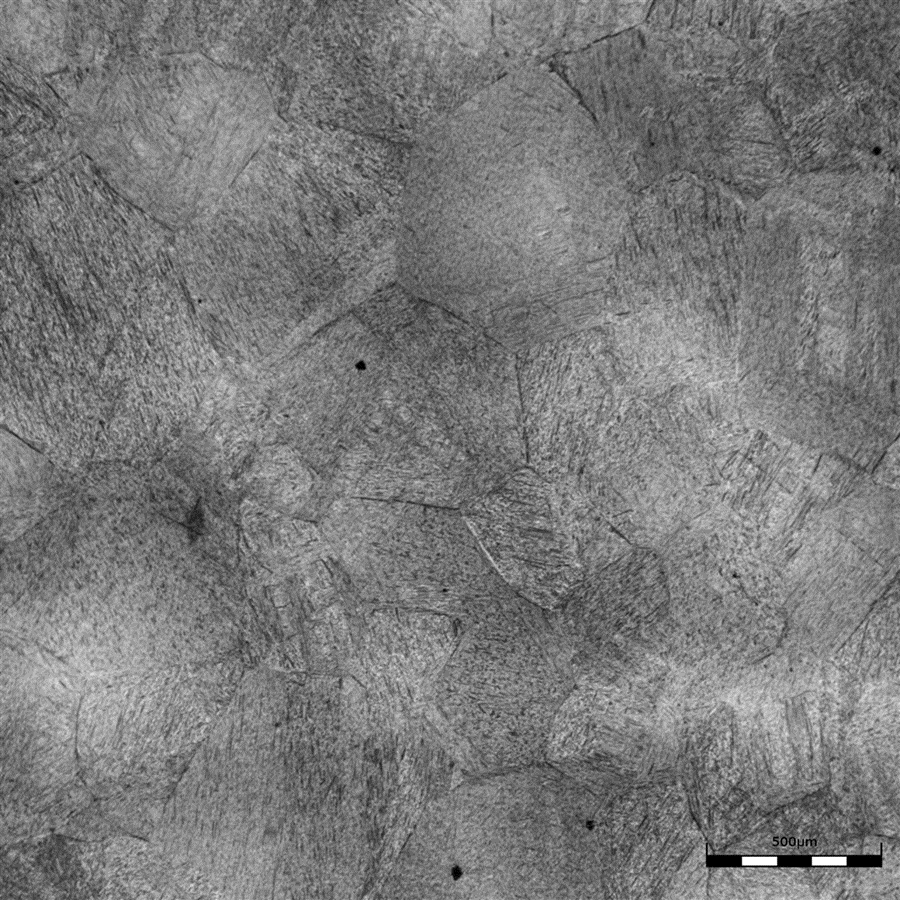
\includegraphics[width=0.9\columnwidth]
{newFigures/BeforeCompM}
\caption{Optical micrograph of the AISI P20 steel before hot compression held during $5$ minutes at $1260^\circ$C}
\label{fig:BeforeCompM}
\end{figure}
\begin{figure}[!ht]
\centering
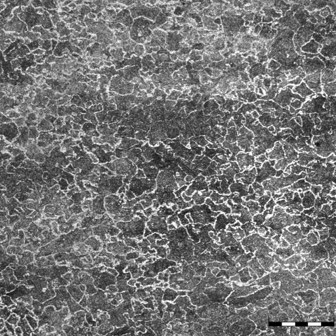
\includegraphics[width=0.9\columnwidth]
{newFigures/AfterCompM}
\caption{Optical micrograph of AISI P20 alloy after howt compression with a strain rate $0.001\ \text{s}^{-1}$ under $1150^\circ$C.}
\label{fig:AfterCompM}
\end{figure}
%-------------------------------------------------------------------------
\subsection{Analytical constitutive flow laws}
%-------------------------------------------------------------------------
The complete characterization of the thermomechanical behavior of a material is very important before its use in numerical simulations. This characterization usually involves experimental tests that serve as a basis for the development of constitutive laws. As mentioned in the introduction, many constitutive laws exist today, and selecting one of them based on explicit criteria hinders the development of computational models for new materials. Since the purpose of this work is to compare analytical models with the ANN model in terms of interpolation and extrapolation, it is important to justify the choice of the analytical models presented here among the many that exist in the literature. Among the most widely used analytical models nowadays, the Johnson-Cook (JC) model is the most used due to its simplicity of use linked to the number of its reduced and easy to obtain parameters. It should be noted that it is not the best model but the most integrated in finite element software. Hence the existence of several modified forms of this model. The Zerilli-Armstrong model, and particularly its modified form (MZA), is also widely known since it tries to provide solutions to the shortcomings of the JC model, particularly with regard to the coupling of physical parameters. Hence its use also in this study. In this perspective, the Hansel Spittel model (HS)is also one of the most widely used models in numerical simulation of casting and forging operations as it is integrated in the FORGE software. Also, the method of identifying its parameters is very simple to do as it is done in one step. Of course, it has its limitations as will be shown in the following sections. Furthermore, the Arrhenius model will be used in this study because it is one of the models that not only provides a good prediction of the flow stress but also takes into account the physical parameter Q (the deformation activation energy coefficient) which is of great importance in the study related to the microstructural analysis of materials. Hence its use in the development of analytical models dedicated to the microstructural analysis of materials. The shortcomings of these models were the main motivation for the formulation of the model proposed in this work, the details of which can be found in our previous work.
%-------------------------------------------------------------------------
\subsubsection{Johnson--Cook model\label{sec:JC}}
%-------------------------------------------------------------------------
The JC model as mentioned above, is one of the most widely used analytical models as it can be applied to several materials under different conditions of strain, strain rate and temperature. However, the formulation of this model does not take into account the simultaneous effect of strain, strain rate and temperature. Indeed, it is formulated by describing the effect of each physical parameter (strain, strain rate and temperature) separately as a factor in the mathematical expression of the model. Hence its inability to describe the phenomenon of temperature-induced softening. The equation that describes this model is given as follows:
\begin{equation}
\label{eq: JCmodel}
\sigma^y = \left(A + B\varepsilon^{p^n}\right)\left(1+C\ln\mdot{\varepsilon}^*\right)\left(1-T^{*^m}\right)
\end{equation}
Where $\sigma^y$ is the equivalent stress flow stress, $\varepsilon^p$ is the plastic strain, ($A=\sigma_0$) is the elastic limit of the material, $B$ is the strain hardening's coefficient, $n$ is the strain hardening's exponent. $C$ and $m$ are the material constants that describe the strain rate hardening and thermal softening exponent respectively. $\mdot{\varepsilon}^*$ is the dimensionless strain rate which is given by $\mdot{\varepsilon}^* = \mdot{\varepsilon^p}/\mdot{\varepsilon_0}$. $\mdot{\varepsilon^p}$ and $\mdot{\varepsilon_0}$ are strain rate and reference strain rate respectively. $T^{*^m} = (T-T_0)/(T_m - T_0)$ is homologous temperature where $T, T_m$ and $T_0$ are the déformation temperature, meltinng temperature (1460$^\circ$C in our case) and reference temperature respectively. For the determination of the parameters of the analytical models, the reference values for strain rate and temperature are $2.0$ and $1050^\circ$C respectively and the value of $A$ is $43.0988$ MPa. Here after datailed the steps for determination the JC model parameters.
At the reference strain rate, Equation \ref{eq: JCmodel} becomes:
\begin{equation}
\label{eq: JCbn}
\sigma^y = A + B\varepsilon^{p^n}
\end{equation}
Taking the natural logarithm on both sides of Equation \ref{eq: JCbn} we have:
\begin{equation}
\label{eq:JClog1}
\ln\left(\sigma^y-A\right)= \ln(B) + n\ln\varepsilon^p
\end{equation}
By plotting $\ln(\sigma^y-A)$ \versus $\ln\varepsilon^p$ (Figure \ref{fig:JCSigmaAB}) from Equation \ref{eq:JClog1}, $n$ and $B$ can be obtained as slope and intercept respectively. Thus, for a strain value equal to $0.1$ the values of these two parameters are $n=0.313969$ and $B=114.518$.
\begin{figure}[!ht]
\centering
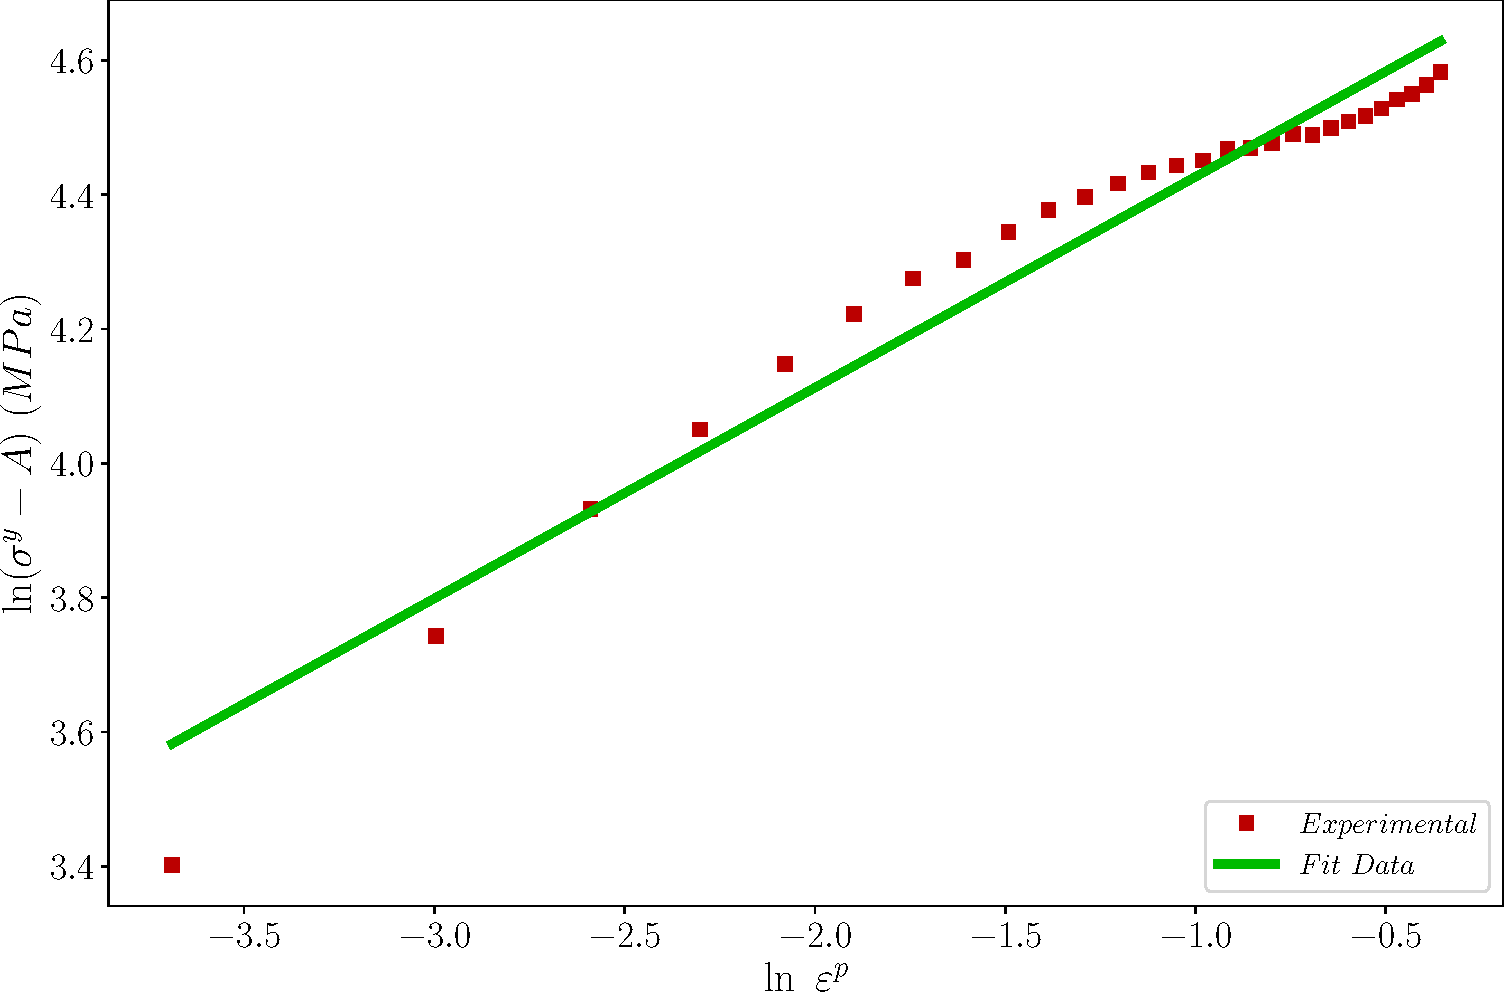
\includegraphics[width=0.9\columnwidth]
{newFigures/JCSigmaAB}
\caption{Relationship between $ln(\sigma^y -A)$ and $\ln(\varepsilon^p)$ at $1050^\circ$C and $0.1$}
\label{fig:JCSigmaAB}
\end{figure}
\FloatBarrier
Once the parameters $A$, $B$ and $n$ are known and at the reference temperature, the Equation \ref{eq: JCmodel} becomes:
\begin{equation}
\frac{\sigma^y}{A + B\varepsilon^{p^n}} = 1 + C\ln\mdot{\varepsilon}^*
\end{equation}
From this equation one can easily obtain the parameter $C$ using the linear fitting method for each strain value and averaging all these values as shown in Figure \ref{fig:JCSigmaAB1} the value is $0.0976681$. 
\begin{figure}[!ht]
\centering
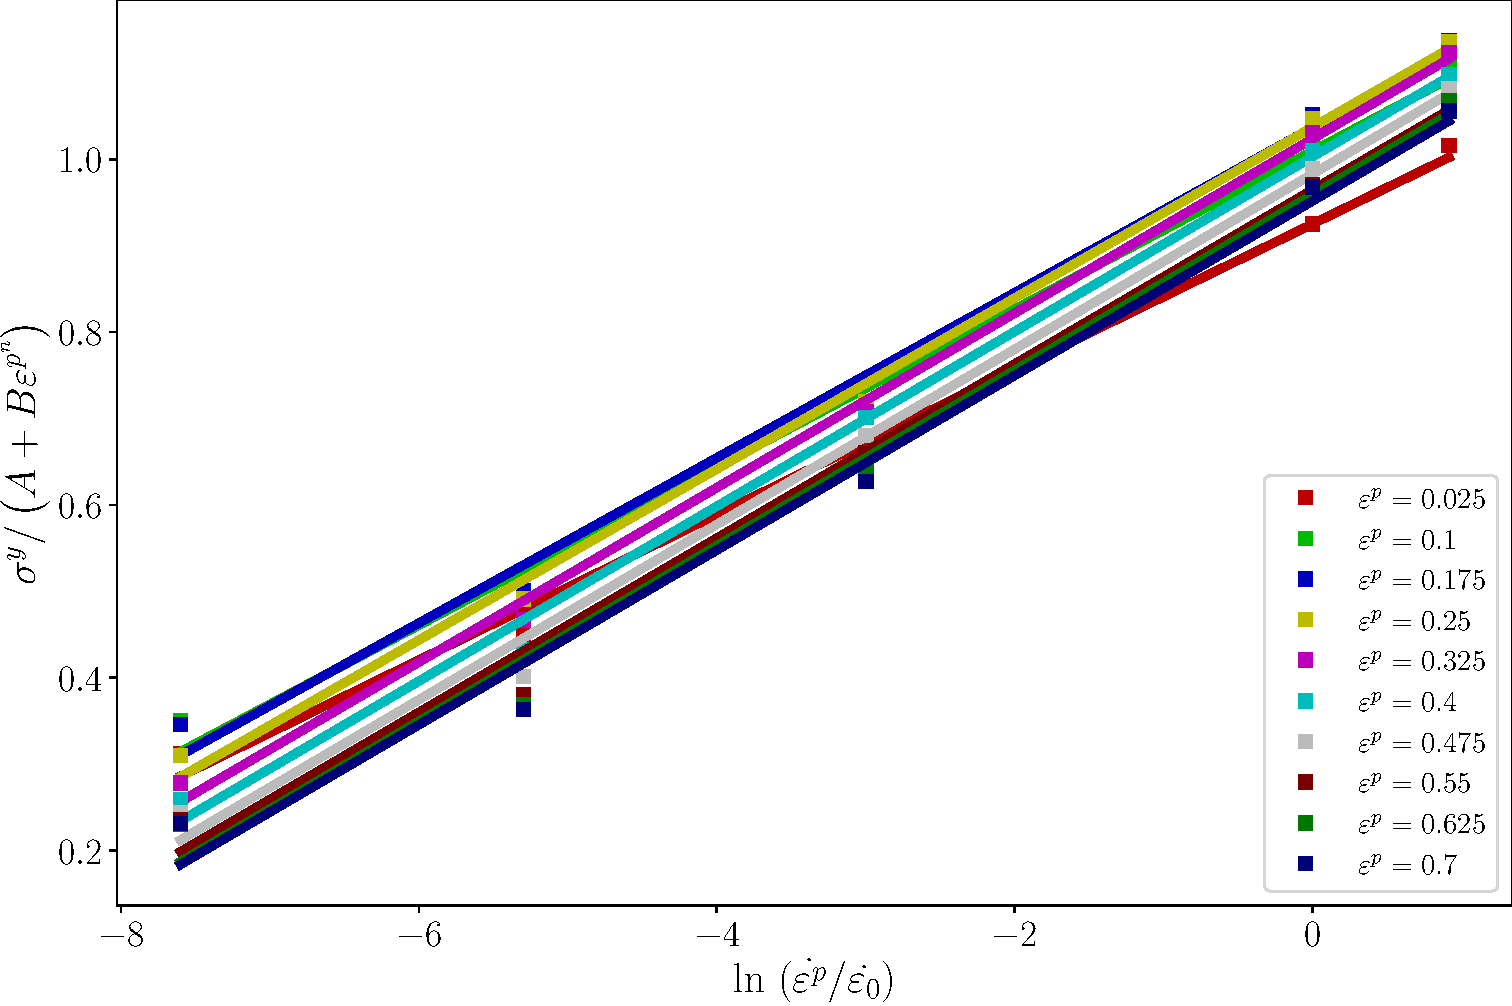
\includegraphics[width=0.9\columnwidth]
{newFigures/JCSigmaAB1}
\caption{Relationship between $\sigma^y/(A+ B\varepsilon^{p^n})$ and $\ln(\dot{\varepsilon}^*)$}
\label{fig:JCSigmaAB1}
\end{figure}
The $m$ parameter is determined at the reference strain rate. Under this condition, the Equation \ref{eq: JCmodel} can be written as following:
\begin{equation}
\frac{\sigma^y}{A + B\varepsilon^{p^n}} = 1 - T^{*^m}
\end{equation}
Taking the natural logarithm of both sides of that equation, we have:
\begin{equation}
\ln\left(1 - \frac{\sigma^y}{A + B\varepsilon^{p^n}}\right)  = m\ln T^*
\end{equation}
Plotting $\ln\left(1 - \frac{\sigma^y}{A + B\varepsilon^{p^n}}\right)$ as a function of $\ln T^*$ allows us to get the parameter $m$ as a slope for all values of the deformation by averaging them and the value is $0.898932$. Figure \ref{fig:JCSigmaT} illustrates this determination for some deformations.
\begin{figure}[!ht]
\centering
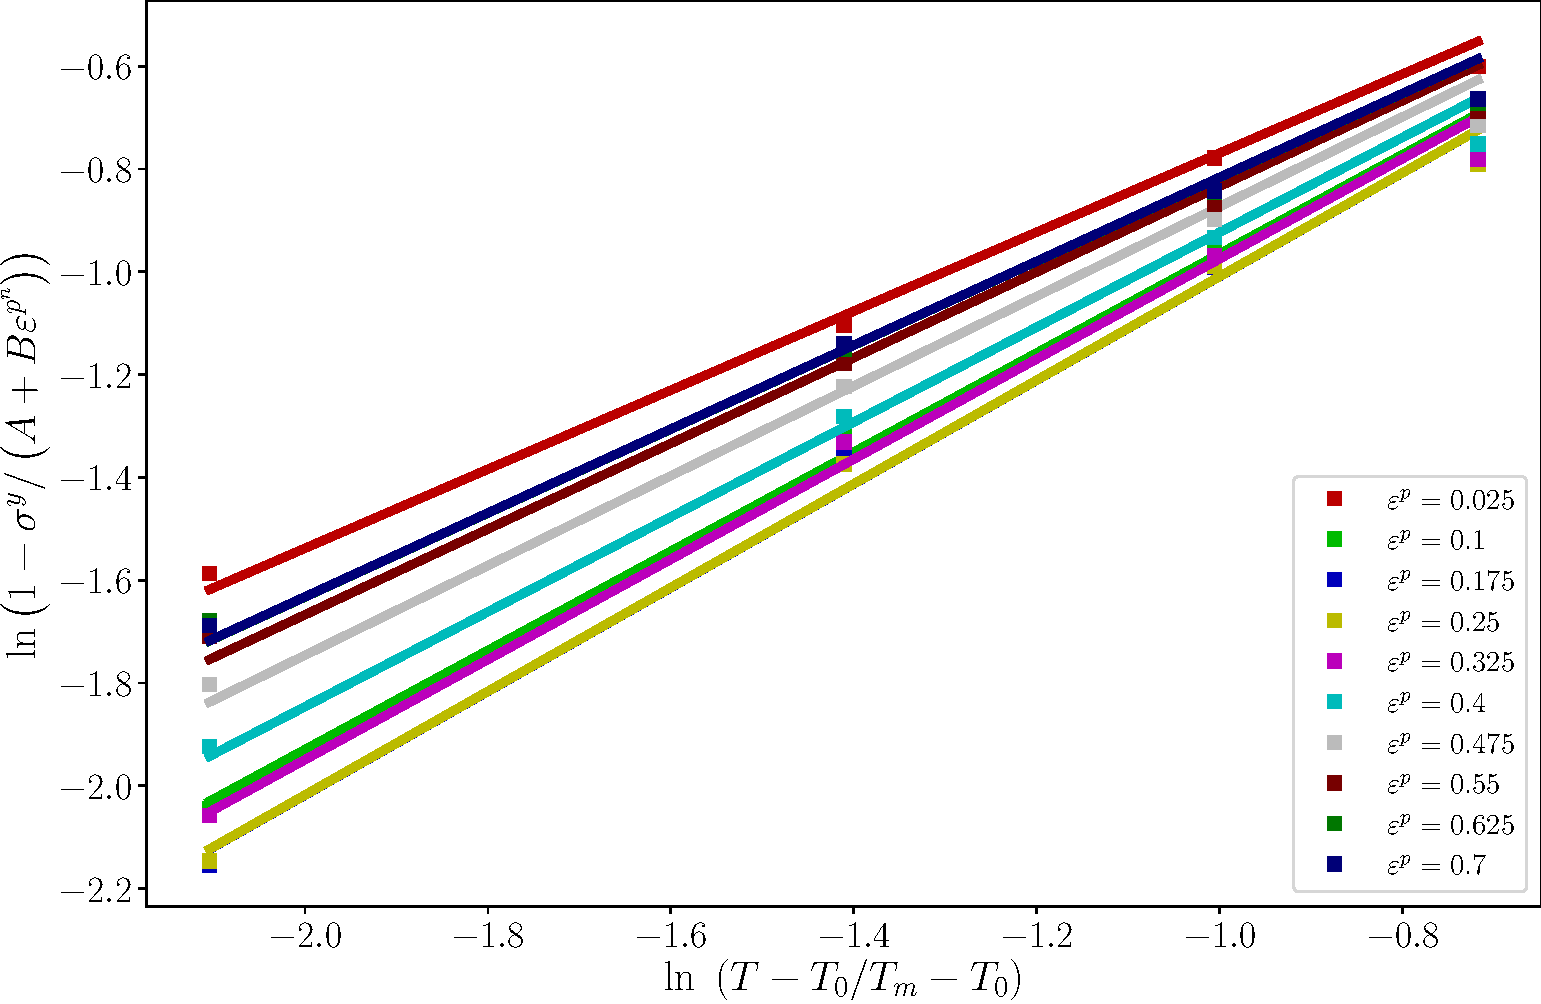
\includegraphics[width=0.85\columnwidth]
{newFigures/JCSigmaT}
\caption{Relationship between $\ln\left(1 - \sigma^y/\left(A + B\varepsilon^{p^n}\right)\right)$ and $\ln T^*$}
\label{fig:JCSigmaT}
\end{figure}
Having determined all the parameters of the Johnson--Cook model, its mathematical formulation can be written as follows:
\begin{equation}
\label{eq: JCmodelf}
\sigma^y = \left(43.0988 + 114.518\varepsilon^{p^{0.313969}}\right)\left(1+0.0976681\ln\mdot{\varepsilon}^*\right)\left(1-T^{*^{0.898932}}\right)
\end{equation}
The predicted and experimental values are compared, as shown in Figure \ref{fig:iCorrelationJC} and Figure  \ref{fig:eCorrelationJC}. The JC model is not much suitable to describe the flow behavior of AISI P20 within entire deformation condition, and predicted values show a monotonous downward trend at various strain rates. The deviation between predicted values and experimental values is large for the low strain rates and almost acceptable at high strain rates.
\begin{figure}[!ht]
\centering
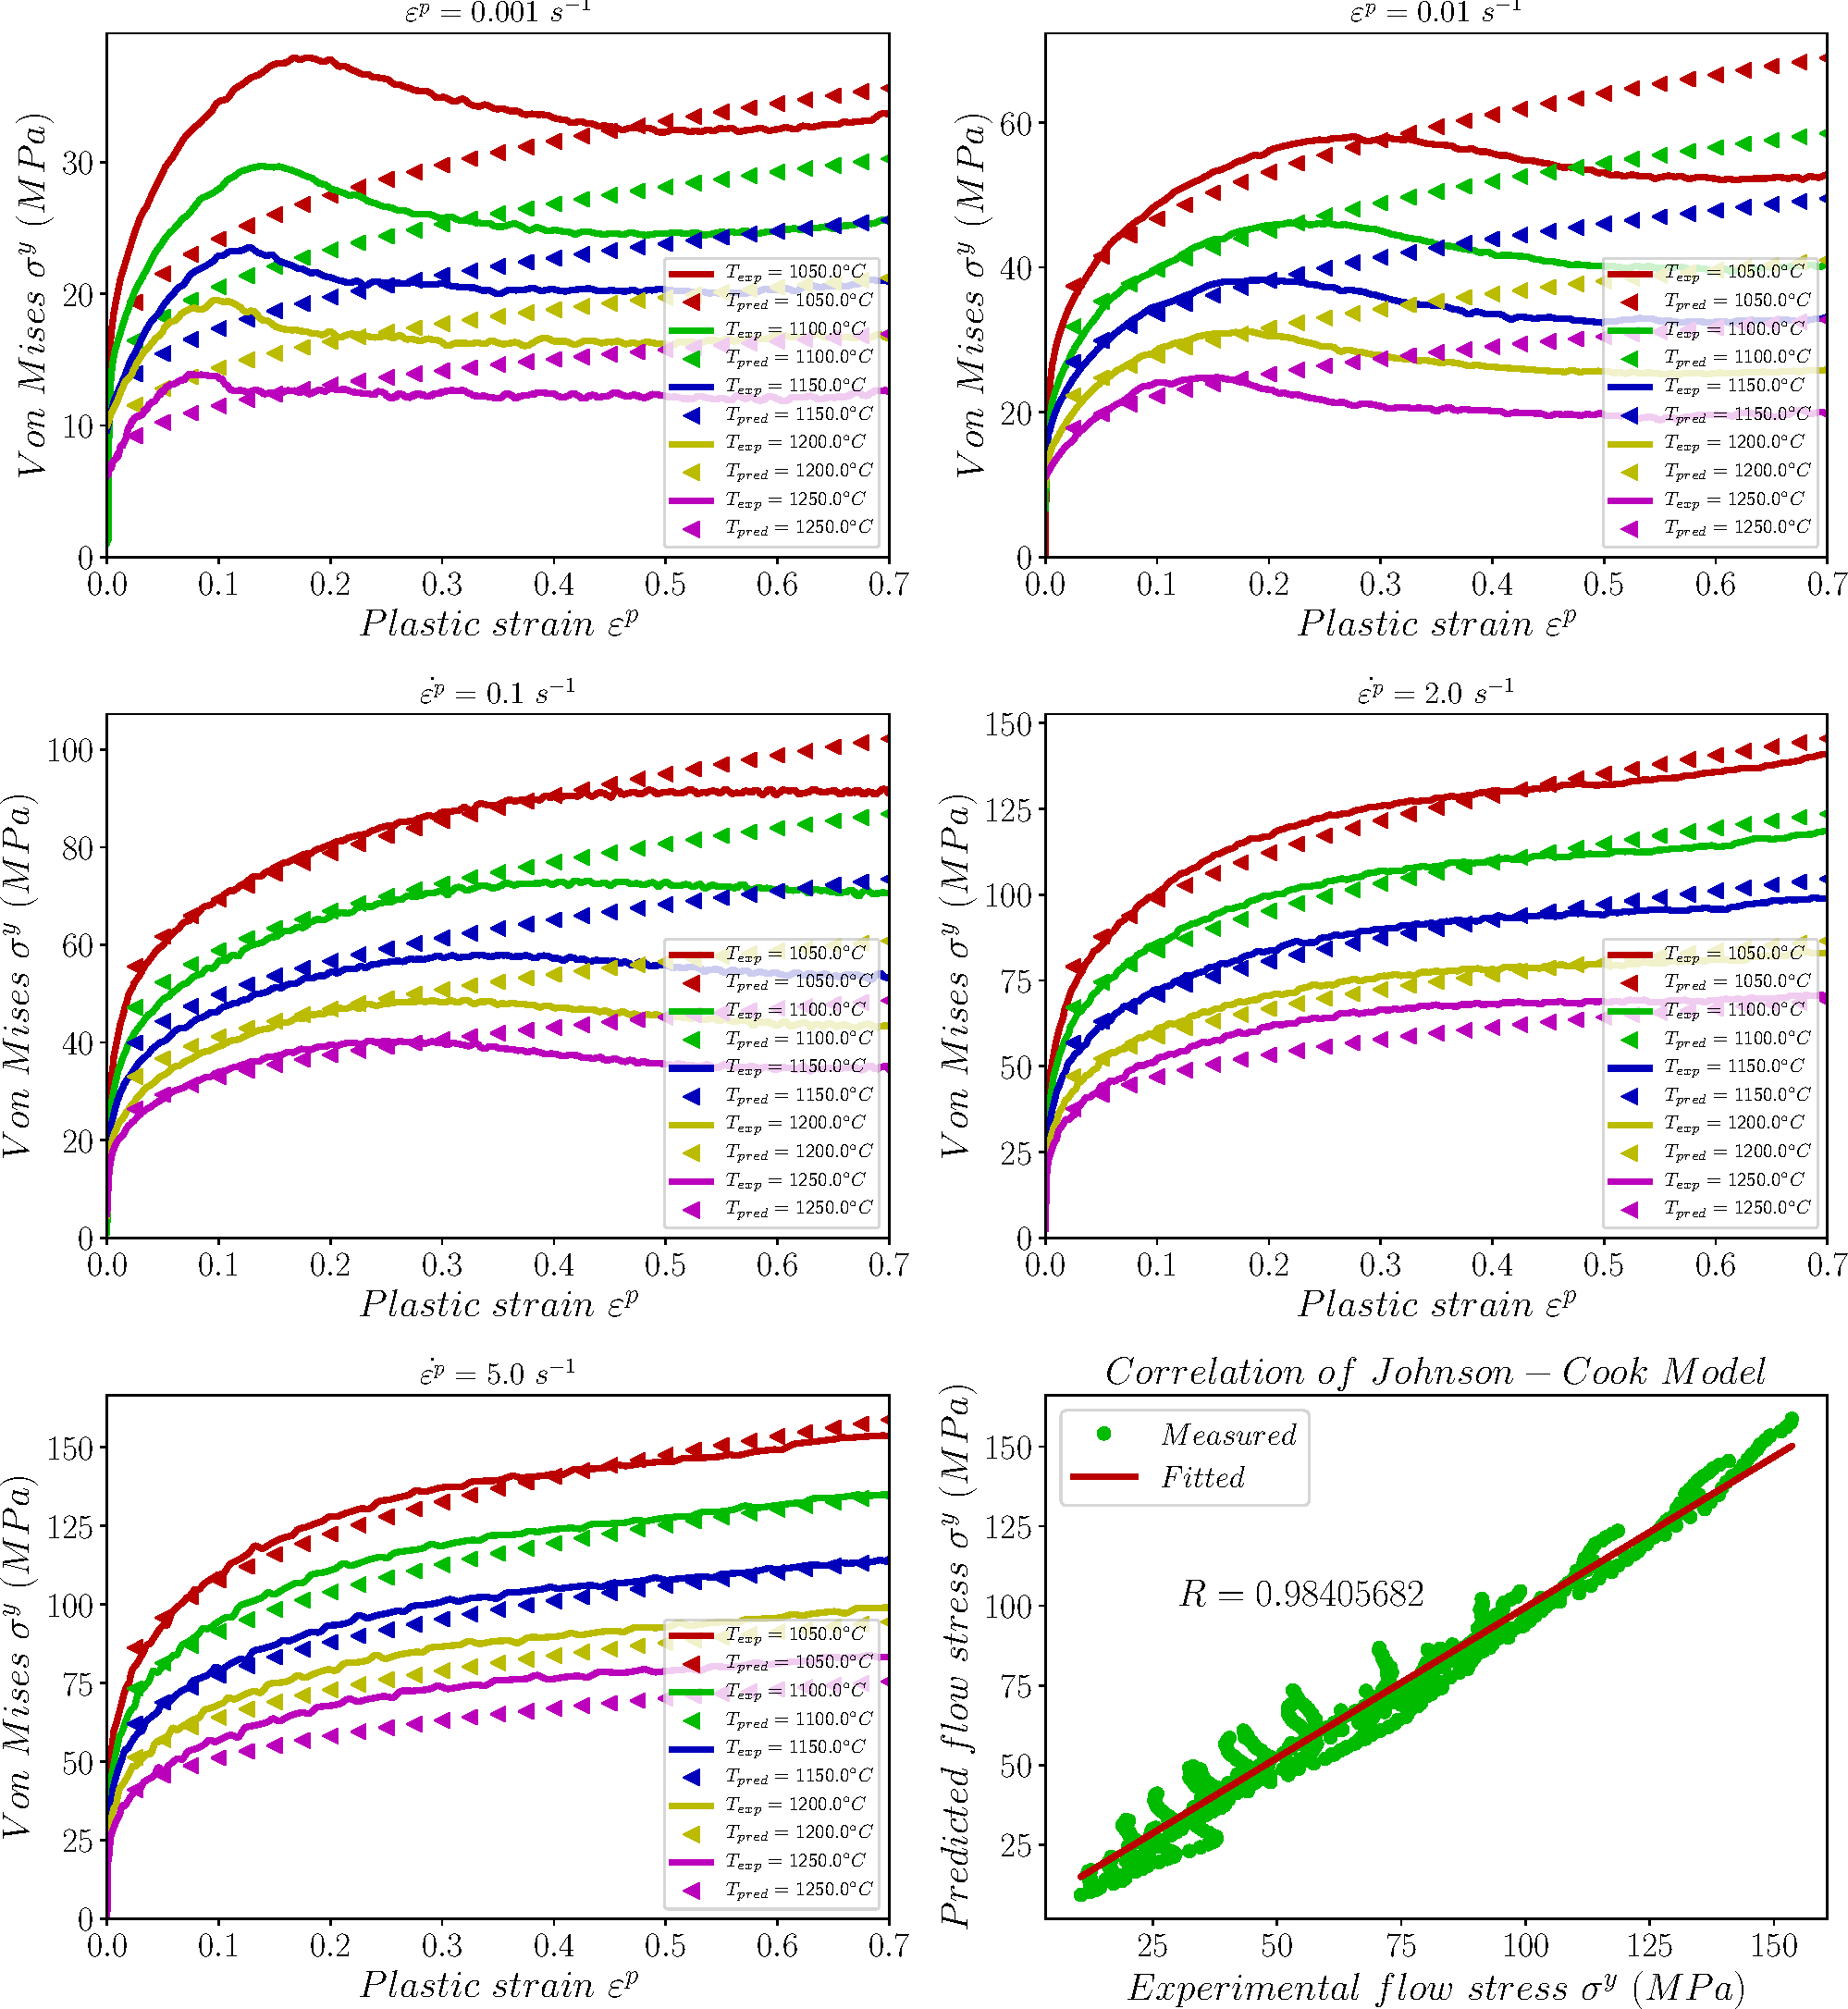
\includegraphics[width=1.02\columnwidth]
{newFigures/iCorrelationJC}
\caption{Comparison between the experimental and predicted flow stresses by JC model for interpolation estimation}
\label{fig:iCorrelationJC}
\end{figure}
\begin{figure}[!ht]
\centering
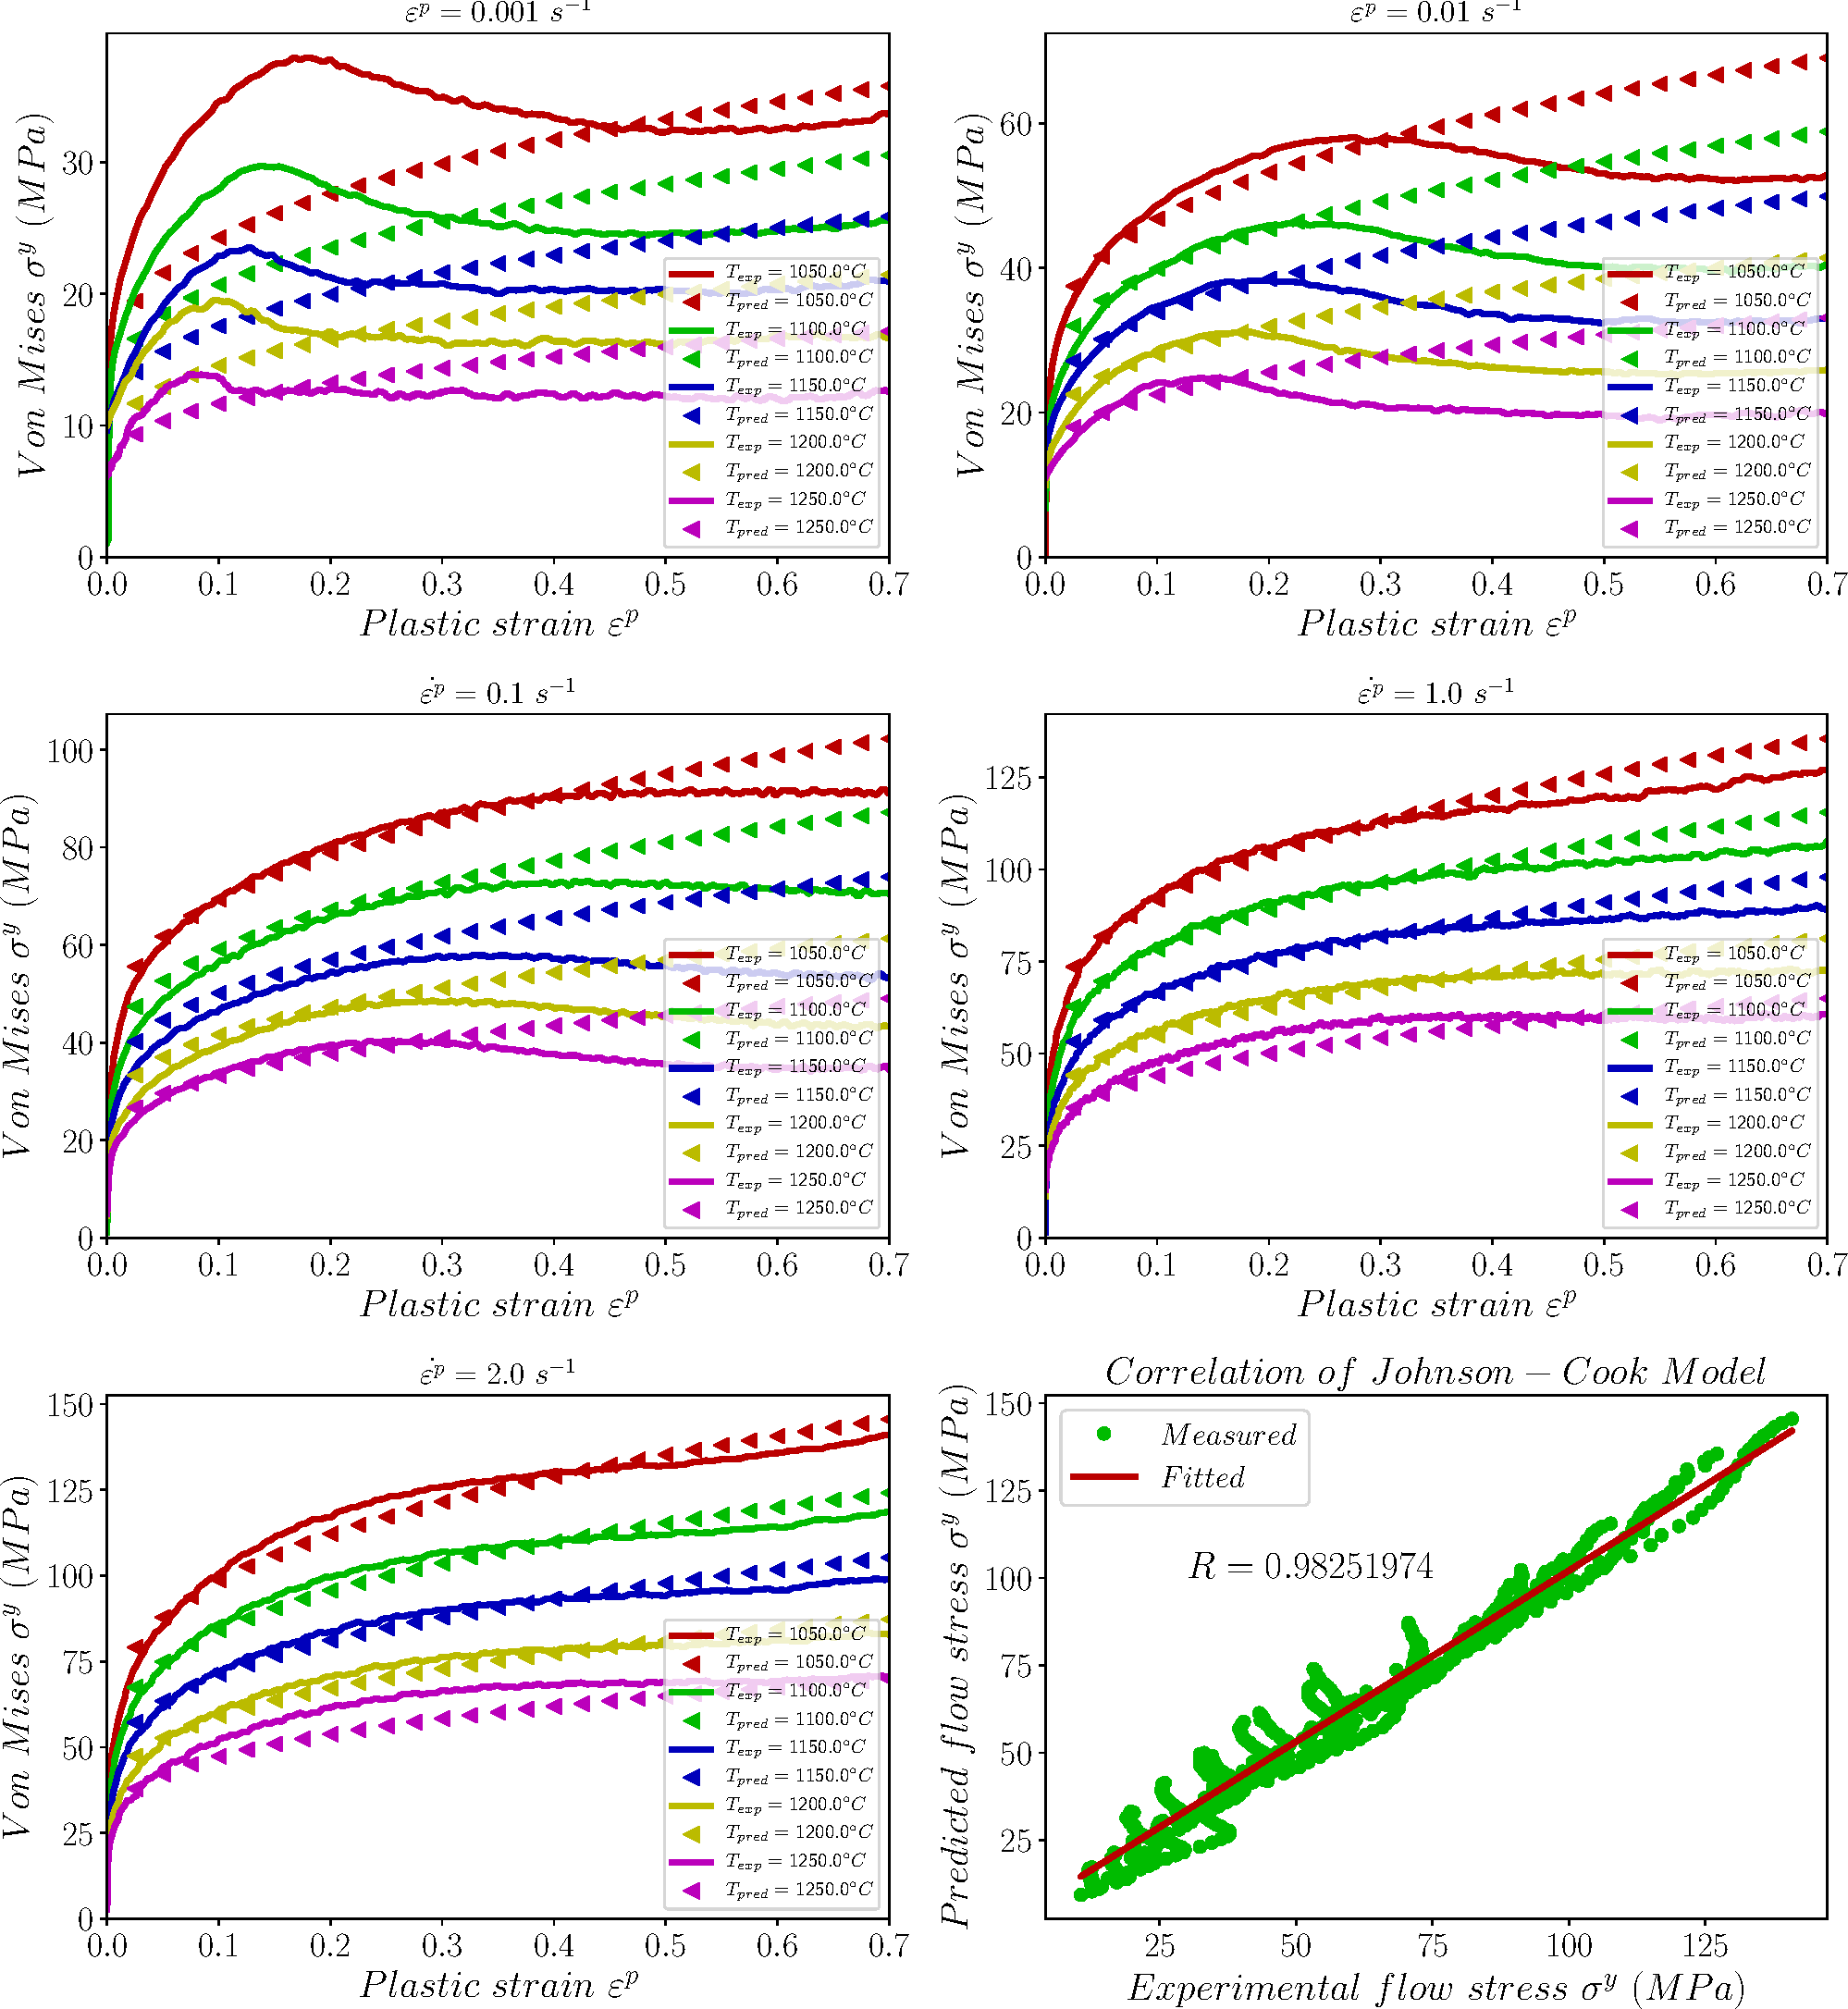
\includegraphics[width=1.02\columnwidth]
{newFigures/eCorrelationJC}
\caption{Comparison between the experimental and predicted flow stresses by JC model for extrapolation estimation}
\label{fig:eCorrelationJC}
\end{figure}
\begin{table}[h!]
\centering{}
\caption{Parameters' constants of Johnson-Cook Model}
\scalebox{1.2}{
\begin{tabular}{lccccc}
\hline
&         &             &		   &		  &\\
&$A(\text{MPa})$    &$B(\text{MPa})$        & $n$     & $C$   & $m$       \\
&         &             &		   &	     &	    \\
\hline
Interpolation&$43.0988$&$114.518$& $0.313969$&$0.0993506$&$0.898932$\\
%\hdashline
Extrapolation&$43.0988$&$114.518$& $0.313969$&$0.0992144$&$0.910297$\\
\hline
\label{tab: JCparameters}
\end{tabular}}
\end{table}
%-------------------------------------------------------------------------
\subsubsection{The Modified Zerilli--Armstrong model\label{sec:MZA}}
%-------------------------------------------------------------------------

As mentioned earlier, Johnson--Cook's law, widely used in the scientific community and implemented as a base in the Abaqus FEM code, is an empirical model for which the effects of strain, strain rate, and temperature on material behavior are considered separately. Since a coupling exists in reality between these three variables, it is preferable to opt for a Zerilli--Armstrong (ZA) model. In fact, the Zerilli--Armstrong model is based on a physical consideration of heat-activated dislocation motion and the interaction of individual dislocations with each other as shown by Hull \eal \cite{Hull-2011-ITD}. The ZA model is therefore a constitutive law based on a study of the material microstructure. For a FCC material, the original equation describing the Zerilli--Armstrong model \cite{Zerilli-1987-DMB} is given by:
\begin{equation}
\label{eq:ZA-model}
\sigma^y = A_{0} + A_{1}\varepsilon^{p^n} \exp\left[-A_{2}T + A_{3}T\ln\left( \frac{\mdot{\varepsilon}^p}{\mdot{\varepsilon}_0}\right)\right]
\end{equation}
where $\sigma^y$ is the von Mises flow stress, $\varepsilon^p$ is the equivalent plastic strain, $\mdot{\varepsilon}^p$ is the equivalent plastic strain rate, $\mdot{\varepsilon}_0$ is the reference strain rate and $T$ is the absolute temperature within the material. The coefficients $A_0$, $A_1$, $A_2$, $A_3$ and $n$ are the parameters of the model to be identified for a given material and $\mdot{\varepsilon}_0$ is the reference strain rate as proposed by many models in the literature.
It is important to note that this model is globally split in two terms. The first term is a constant stress threshold representing the yield strength of the material and the second term is a thermo-viscous component considering the variation of the work hardening threshold of the material with temperature and strain rate.
With face-centered cubic (FCC) materials, the strain hardening shows a greater dependence on both temperature and strain rate. The thermal component of strain hardening in FCC materials is physically interpreted as the resistance to dislocation motion by the mutual interaction of dislocations \cite{Voyia-2005-MBM}. The flow stress threshold of an FCC material is independent of temperature and strain rate, so that the flow stress threshold is constant and equal to the initial stress \cite{Nemat-2004-Plasticity, Voyia-2005-MBM}. The limitation of the ZA model is that it cannot be used for flow stress prediction at high strain rates and temperatures above $0.6~T_m$. To circumvent this problem, Samantaray \eal \cite{Samantaray-2009-Thermo-viscoplastic} proposed a modified form of the Zerilli--Armstrong law (MZA) given by the following relationship:
\begin{equation}
\label{eq:MZA-model}
\sigma^y = \left(C_{1}+C_{2}\varepsilon^{p^n}\right) \exp\left[-\left(C_{3}+C_{4}\varepsilon^p\right)\left(T-T_0\right) + \left(C_{5}+C_{6}\left(T-T_0\right)\right)\ln\left( \frac{\mdot{\varepsilon}^p}{\mdot{\varepsilon}_0}\right)\right]
\end{equation}
where the $7$ coefficients $C_i$ and $n$ are the parameters of the model to be identified for a given material. This formulation was initially developed from a compression test of 15Cr--15Ni--2.2Mo Ti-modified austenitic stainless steel (the D9 alloy). This test was performed over a range of plastic strains ($\varepsilon^p=0.1-0.5$), strain rates ($\mdot{\varepsilon}^p=10^{-3}-1~\text{s}^{-1}$) and temperatures ($T=800-1200^\circ\text{C}$). In attempting to apply the original Johnson--Cook model, the authors of this work found that it was unable to describe the behavior of this type of material over the ranges of strain, strain rate, and temperature mentioned above. The same conclusion was made regarding the ZA model who was also unable to correctly describe the behavior of this material. Based on the ZA model, Samantaray \eal \cite{Samantaray-2009-Thermo-viscoplastic} have therefore proposed a modified form of the ZA model to better describe the behavior of this material. This modified model takes into account the effect of isotropic strain hardening, strain rate hardening, thermal softening and the coupled effects of strain, strain rate and temperature on the flow stress. It predicts the evolution of the high-temperature flow threshold of the D9 alloy over the above ranges of strain, strain rate and temperature with good correlation to the experimental data and good generalization. The correlation coefficient obtained is $0.995$ while the average error for the whole data set is only $5.3~\%$. For more details about the formulation of this model the author can read \cite{Samantaray-2009-Thermo-viscoplastic}.

The Equation (\ref{eq:ZA-model}) of the original Zerilli--Armstrong model defines the flow stress in two terms: a thermal stress and an athermal stress that depends on the grain size of the material and is independent of temperature. However, several studies have shown that this independence decreases when the temperature increases beyond a certain value. Based on these observations, Samantaray questioned the athermal consideration for the D9 material. This approach then allows for the consideration of temperature effects on the yield strength of D9 steel and even other materials. Here after how to get all parameters of the MZA model:

Considering the expression of the model given by Equation (\ref{eq:MZA-model}), parameter $C_1$ is deduced direcly from $\sigma^y(\varepsilon^p=0,T=T_0,\mdot{\varepsilon}^p=\mdot{\varepsilon}_0)$. When the current strain rate $\mdot{\varepsilon}^p$ is identical to the reference strain rate $\mdot{\varepsilon}_0$, the Equation (\ref{eq:MZA-model}) becomes :
\begin{equation}
\sigma^y = \left(C_{1}+C_{2}\varepsilon^{p^n}\right) \exp\left[-\left(C_{3}+C_{4}\varepsilon^p\right)\left(T-T_0\right)\right]
\end{equation}
Taking the logarithm of the previous relationship we have :
\begin{equation}
\ln\sigma^y = \ln\left(C_{1}+C_{2}\varepsilon^{p^n}\right)-\left(C_{3}+C_{4}\varepsilon^p\right)\left(T-T_0\right)
\end{equation}
By plotting the function $\ln\sigma^y\left(T-T_0\right)$ the y-intercept and the slope of this line can be deduced as $I_1=\ln\left(C_1+C_2\varepsilon^{p^n}\right)$ and $S_1=-\left(C_3+C_4\varepsilon^p\right)$.
From the expression of $I_1$ we can write:
\begin{equation}
\ln\left(\exp(I_1)-C_1\right) = \ln C_2+n\ln\varepsilon^p
\end{equation}
By plotting the function $\ln\left(\exp(I_1)-C_1\right)$ versus $\ln\varepsilon^p$ we can deduce $n$ and $C_2$. The plot of $S_1$ versus $\varepsilon^p$ allows deducing $C_3$ and $C_4$ from the y-intercept and the slope, respectively. Once the first four terms of the model are calculated, we can now take the logarithm of the entire MZA model given by Equation (\ref{eq:MZA-model}).
\begin{equation}
\ln\sigma^y = \ln\left(C_{1}+C_{2}\varepsilon^{p^n}\right) - \left(C_{3}+C_{4}\varepsilon^p\right)\left(T-T_0\right) + S_2\ln\left( \frac{\mdot{\varepsilon}^p}{\mdot{\varepsilon}_0}\right)
\end{equation}
with $S_2=C_5+C_6\left(T-T_0\right)$. Finally, the graph $\ln\sigma^y$ versus $ \ln(\mdot{\varepsilon}^p/\mdot{\varepsilon}_0)$ allows deducing $C_5$ and $C_6$ from the slope $S_2$. The parameters (both the interpolation and extrapolation indentification) of MZA model are given in the Table \ref{tab: MZAparameters} while its prediction are shown in Figure \ref{fig:iCorrelationMZA} and Figure \ref{fig:eCorrelationMZA}. It can be seen from those figures that the MZA model as JC model is not suitable to describe experimental at low strain rates but much better for high strain rates. The deviation between the predicted values and the experimental values is large because this model has problem to correctly describe the softening in its formulation. That is aspect of the limitations of that model as presented in \cite{tize2022generalized}.
\begin{table}[h!]
\centering{}
\caption{Parameters' constants of Modified--Zerrilli-Armstrong Model}
\scalebox{0.83}{
\begin{tabular}{lllllllc}
\hline
&         &             &		   &		 &			   &&\\
&$C_1(\text{MPa})$    &$C_2(\text{MPa})$        & $C_3(\times10^{-5})$     & $C_4(\times10^{-5})$   & $C_5(\times10^{-5})$       &$C_6(\times10^{-5})$&$n$\\
&         &             &		   &	     &	           &&\\
\hline
Interpolation&$43.0988$&$112.975$& $330.976$&$4.27581$&$14036.3$&$17.1520$&$0.305028$\\
%\hdashline
Extrapolation&$43.0988$&$112.975$& $330.976$&$4.27581$&$14496.9
$&$18.9194$&$0.305028$\\
\hline
\label{tab: MZAparameters}
\end{tabular}}
\end{table}
\begin{figure}[!ht]
\centering
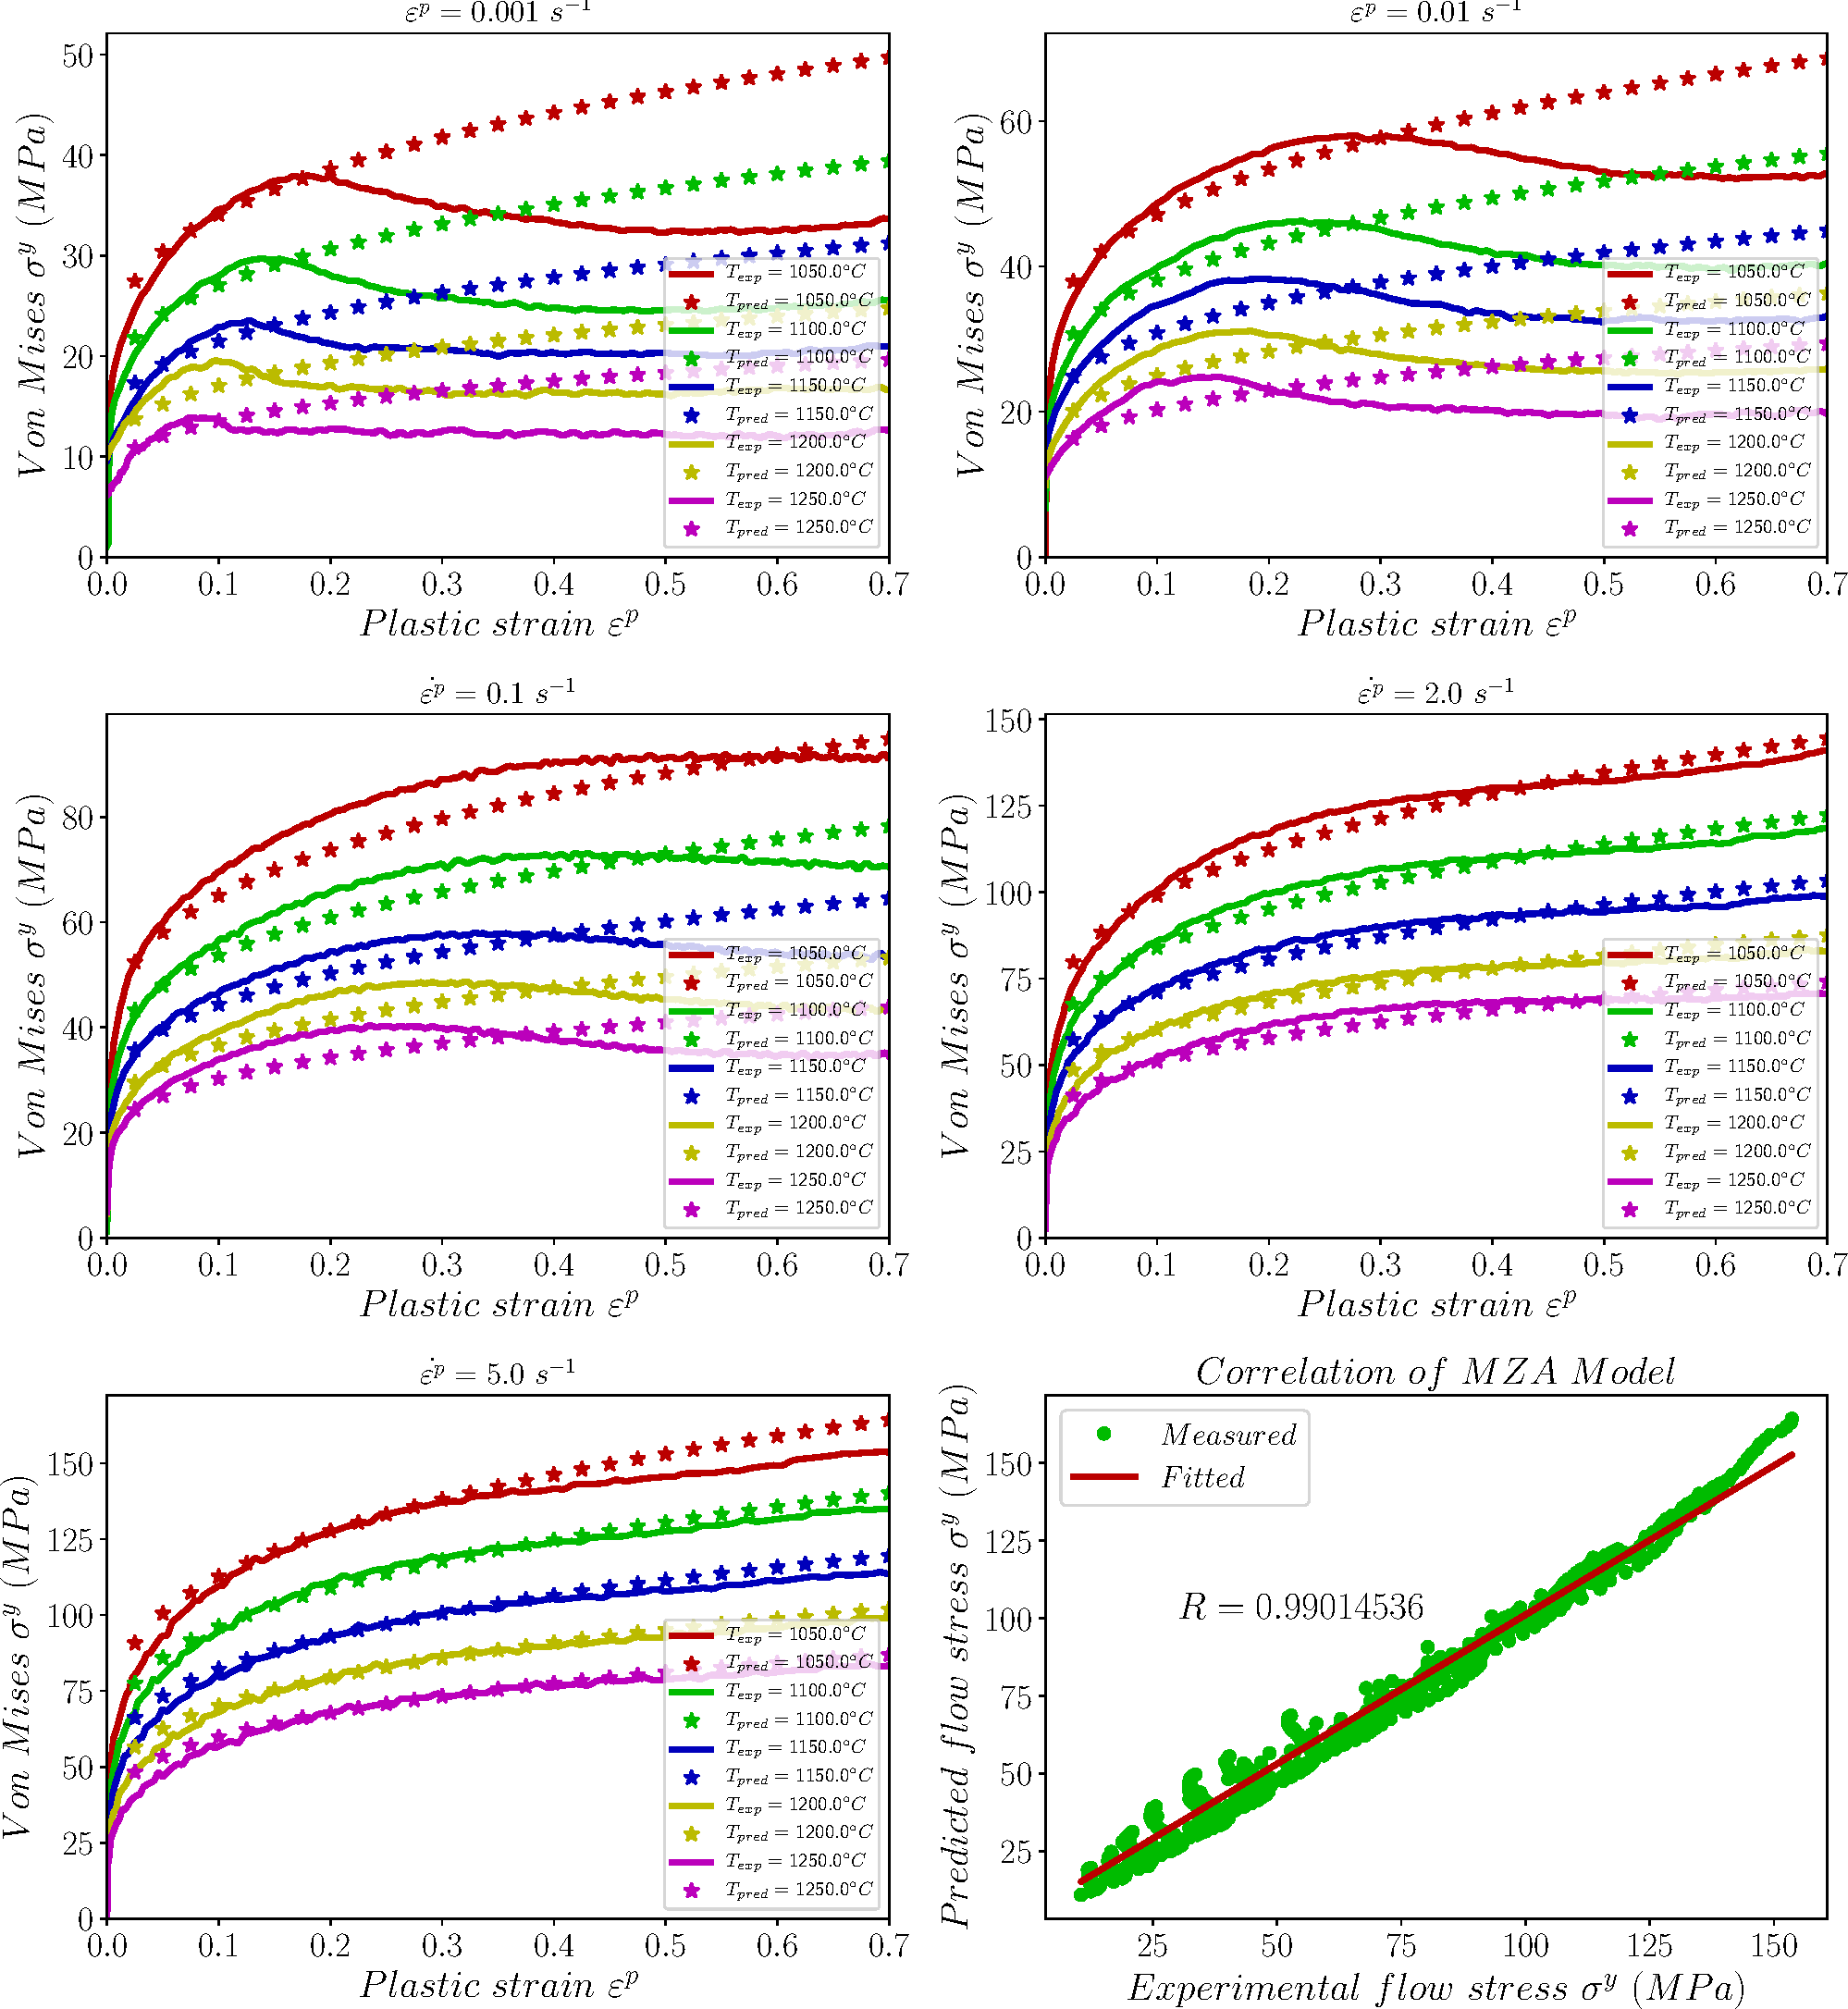
\includegraphics[width=1.02\columnwidth]
{newFigures/iCorrelationMZA}
\caption{Comparison between the experimental and predicted flow stresses by MZA model for interpolation estimation}
\label{fig:iCorrelationMZA}
\end{figure}
\begin{figure}[!ht]
\centering
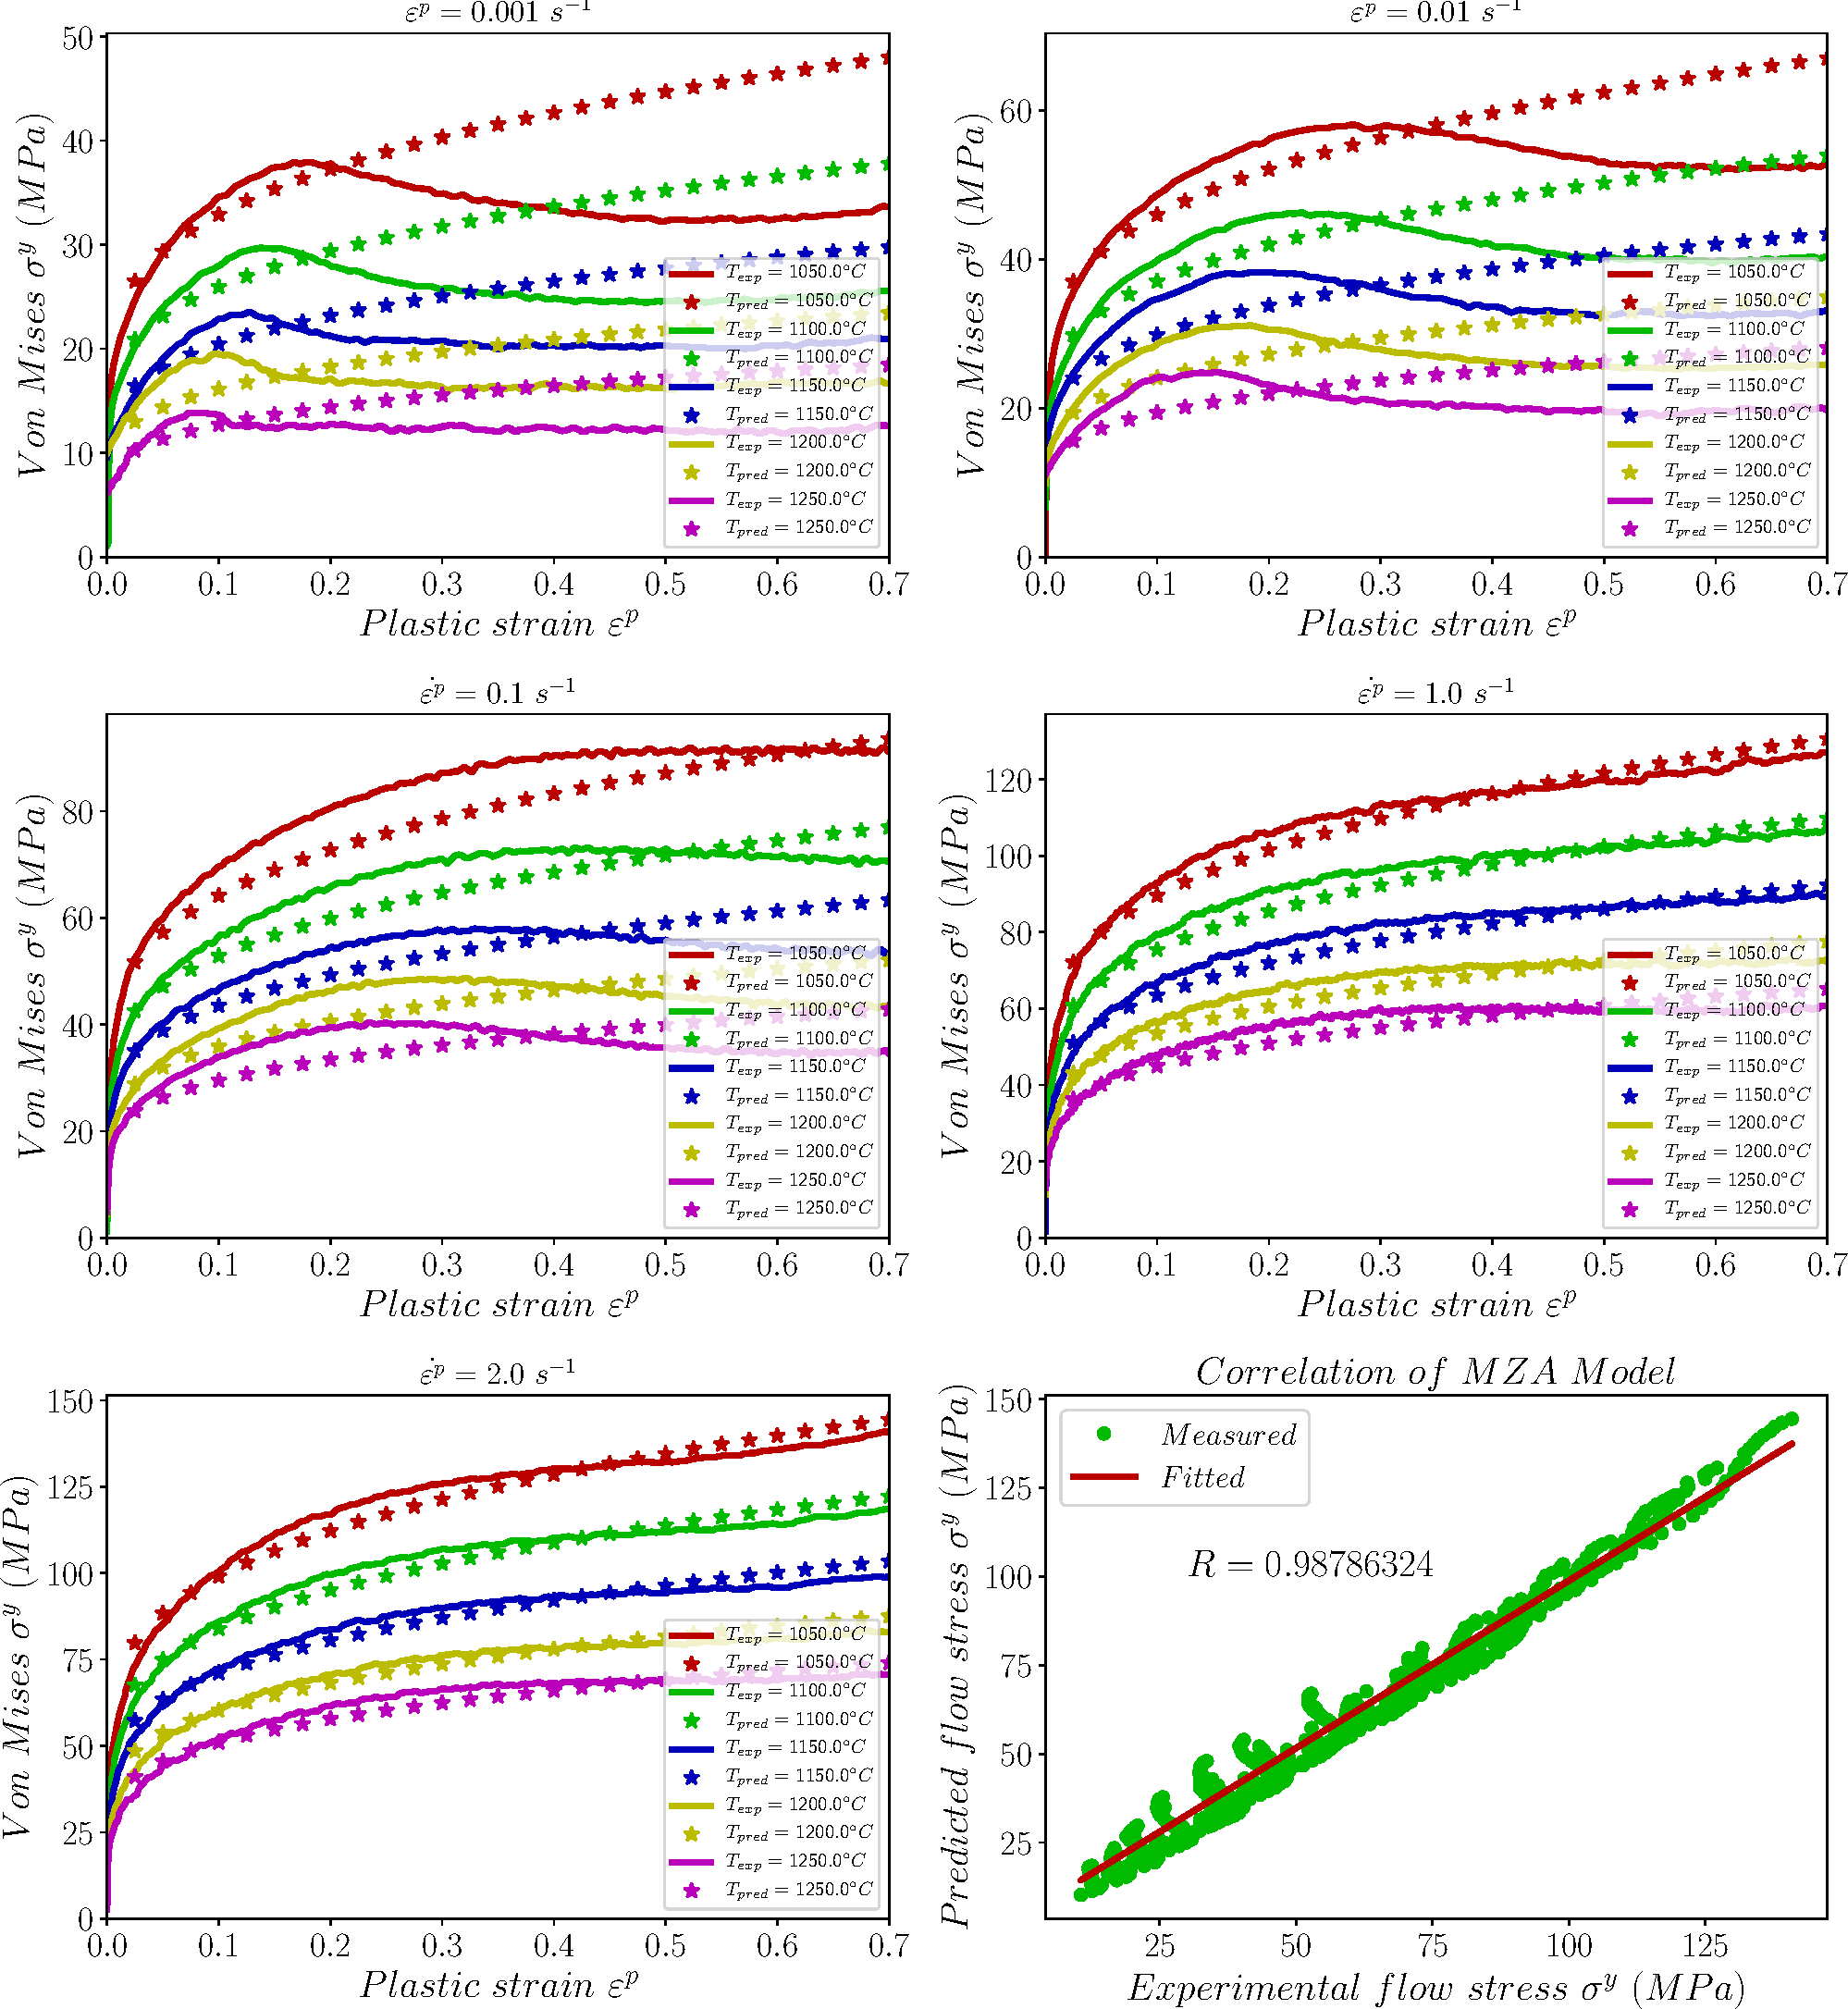
\includegraphics[width=1.02\columnwidth]
{newFigures/eCorrelationMZA}
\caption{Comparison between the experimental and predicted flow stresses by MZA model for extrapolation estimation}
\label{fig:eCorrelationMZA}
\end{figure}
\FloatBarrier

%-------------------------------------------------------------------------
\subsubsection{Hansel and Spittel\label{sec:HSmodel}}
%-------------------------------------------------------------------------
The Hansel-Spittel model is one of the least known models in terms of its  integration in softwae for finite element simulation although the determination of its parameters is easier than the JC model. A single programming command is sufficient for its identification. However, this model has some difficulties as it loses its accuracy when all parameters are taken into account. For this reason, several authors limit its use to $5$ or $6$ parameters \cite{chadha2018approach, rudnytskyj2020constitutive, el2015comparison}. In this paper the good predictions are with $5$ parameters summarized in Table \ref{tab: HSparameters}. The equation of the model is given by the following relation: 
\begin{equation}
\sigma^y = Ae^{m_1T}\varepsilon^{p^{m_2}}\mdot{\varepsilon}^{p^{m_3}}e^{\frac{m_4}{\varepsilon^p}}(1+\varepsilon^p)^{m_5T}e^{m_6\varepsilon^p}\mdot{\varepsilon}^{p^{m_7T}}T^{m_8}
\end{equation}
Where $\sigma^y$ is the flow stess, $\varepsilon^p$ strain, $\mdot{\varepsilon}^p$ strain rate and $T$ temperature. The other coefficients $A$ and $m_j$ are model constants up to $m_5$ for our case. Comparison of predicted values of the HS model and experimental values is shown in Figure \ref{fig:iCorrelationHS} and Figure \ref{fig:eCorrelationHS}. It appears that this model as well as the previous ones do not predict the experimental well and the gap is relatively large. This shows that this model is not appropriate for the characterisation of this alloy.
\begin{table}[h!]
\centering{}
\caption{Parameters' constants of Hansel and Spittel Model}
\scalebox{0.9}{
\begin{tabular}{llccccc}
\hline
&         &             &		   &		 &			   &\\
&$A_0(\text{GPa})$    &$m_1$        & $m_2$     & $m_3$   & $m_4$       &$m_5$\\
&         &             &		   &	     &	           &\\
\hline
Interpolation&$10.1777$&$-0.00384785$& $0.195671$&$0.183171$&$-0.0035643$&$-0.00059302$\\
%\hdashline
Extrapolation&$11.3176$&$-0.00388286$& $0.204999$&$0.19018$&$-0.00316225$&$-0.000658053$\\
\hline
\label{tab: HSparameters}
\end{tabular}}
\end{table}
\begin{figure}[!ht]
\centering
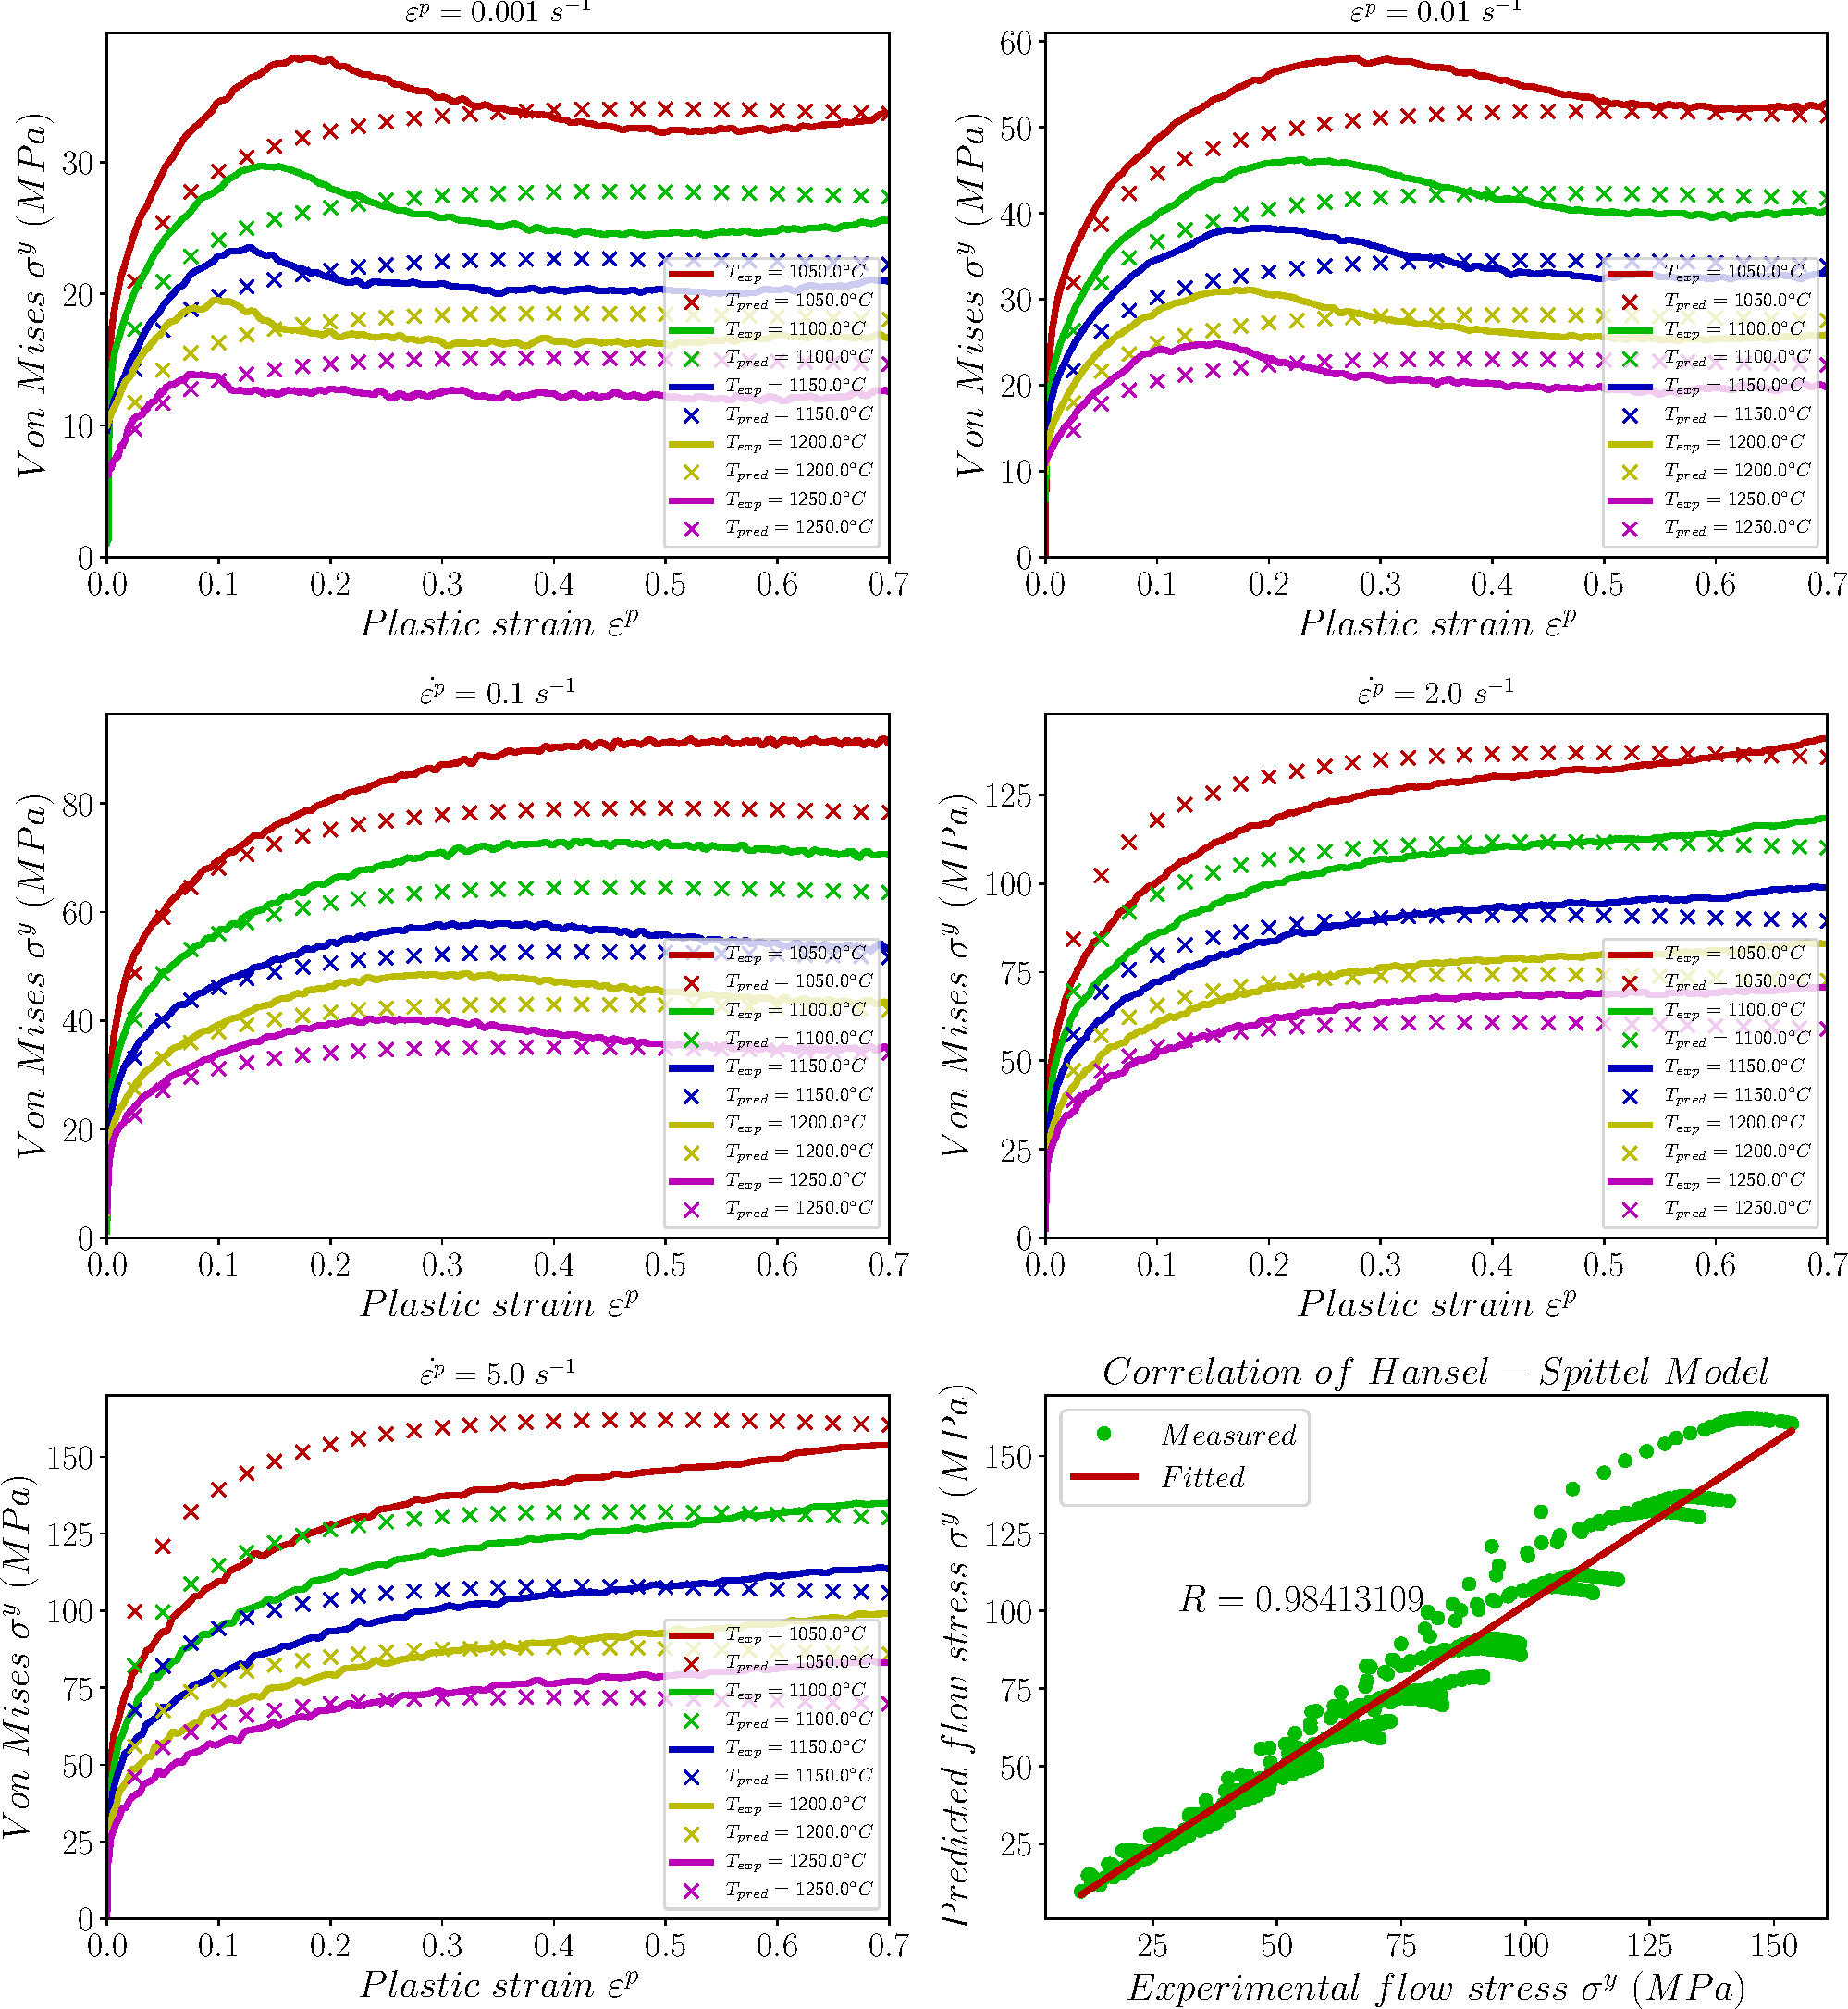
\includegraphics[width=1.02\columnwidth]
{newFigures/iCorrelationHS}
\caption{Comparison between the experimental and predicted flow stresses by HS model for interpolation estimation}
\label{fig:iCorrelationHS}
\end{figure}
\FloatBarrier
\begin{figure}[!ht]
\centering
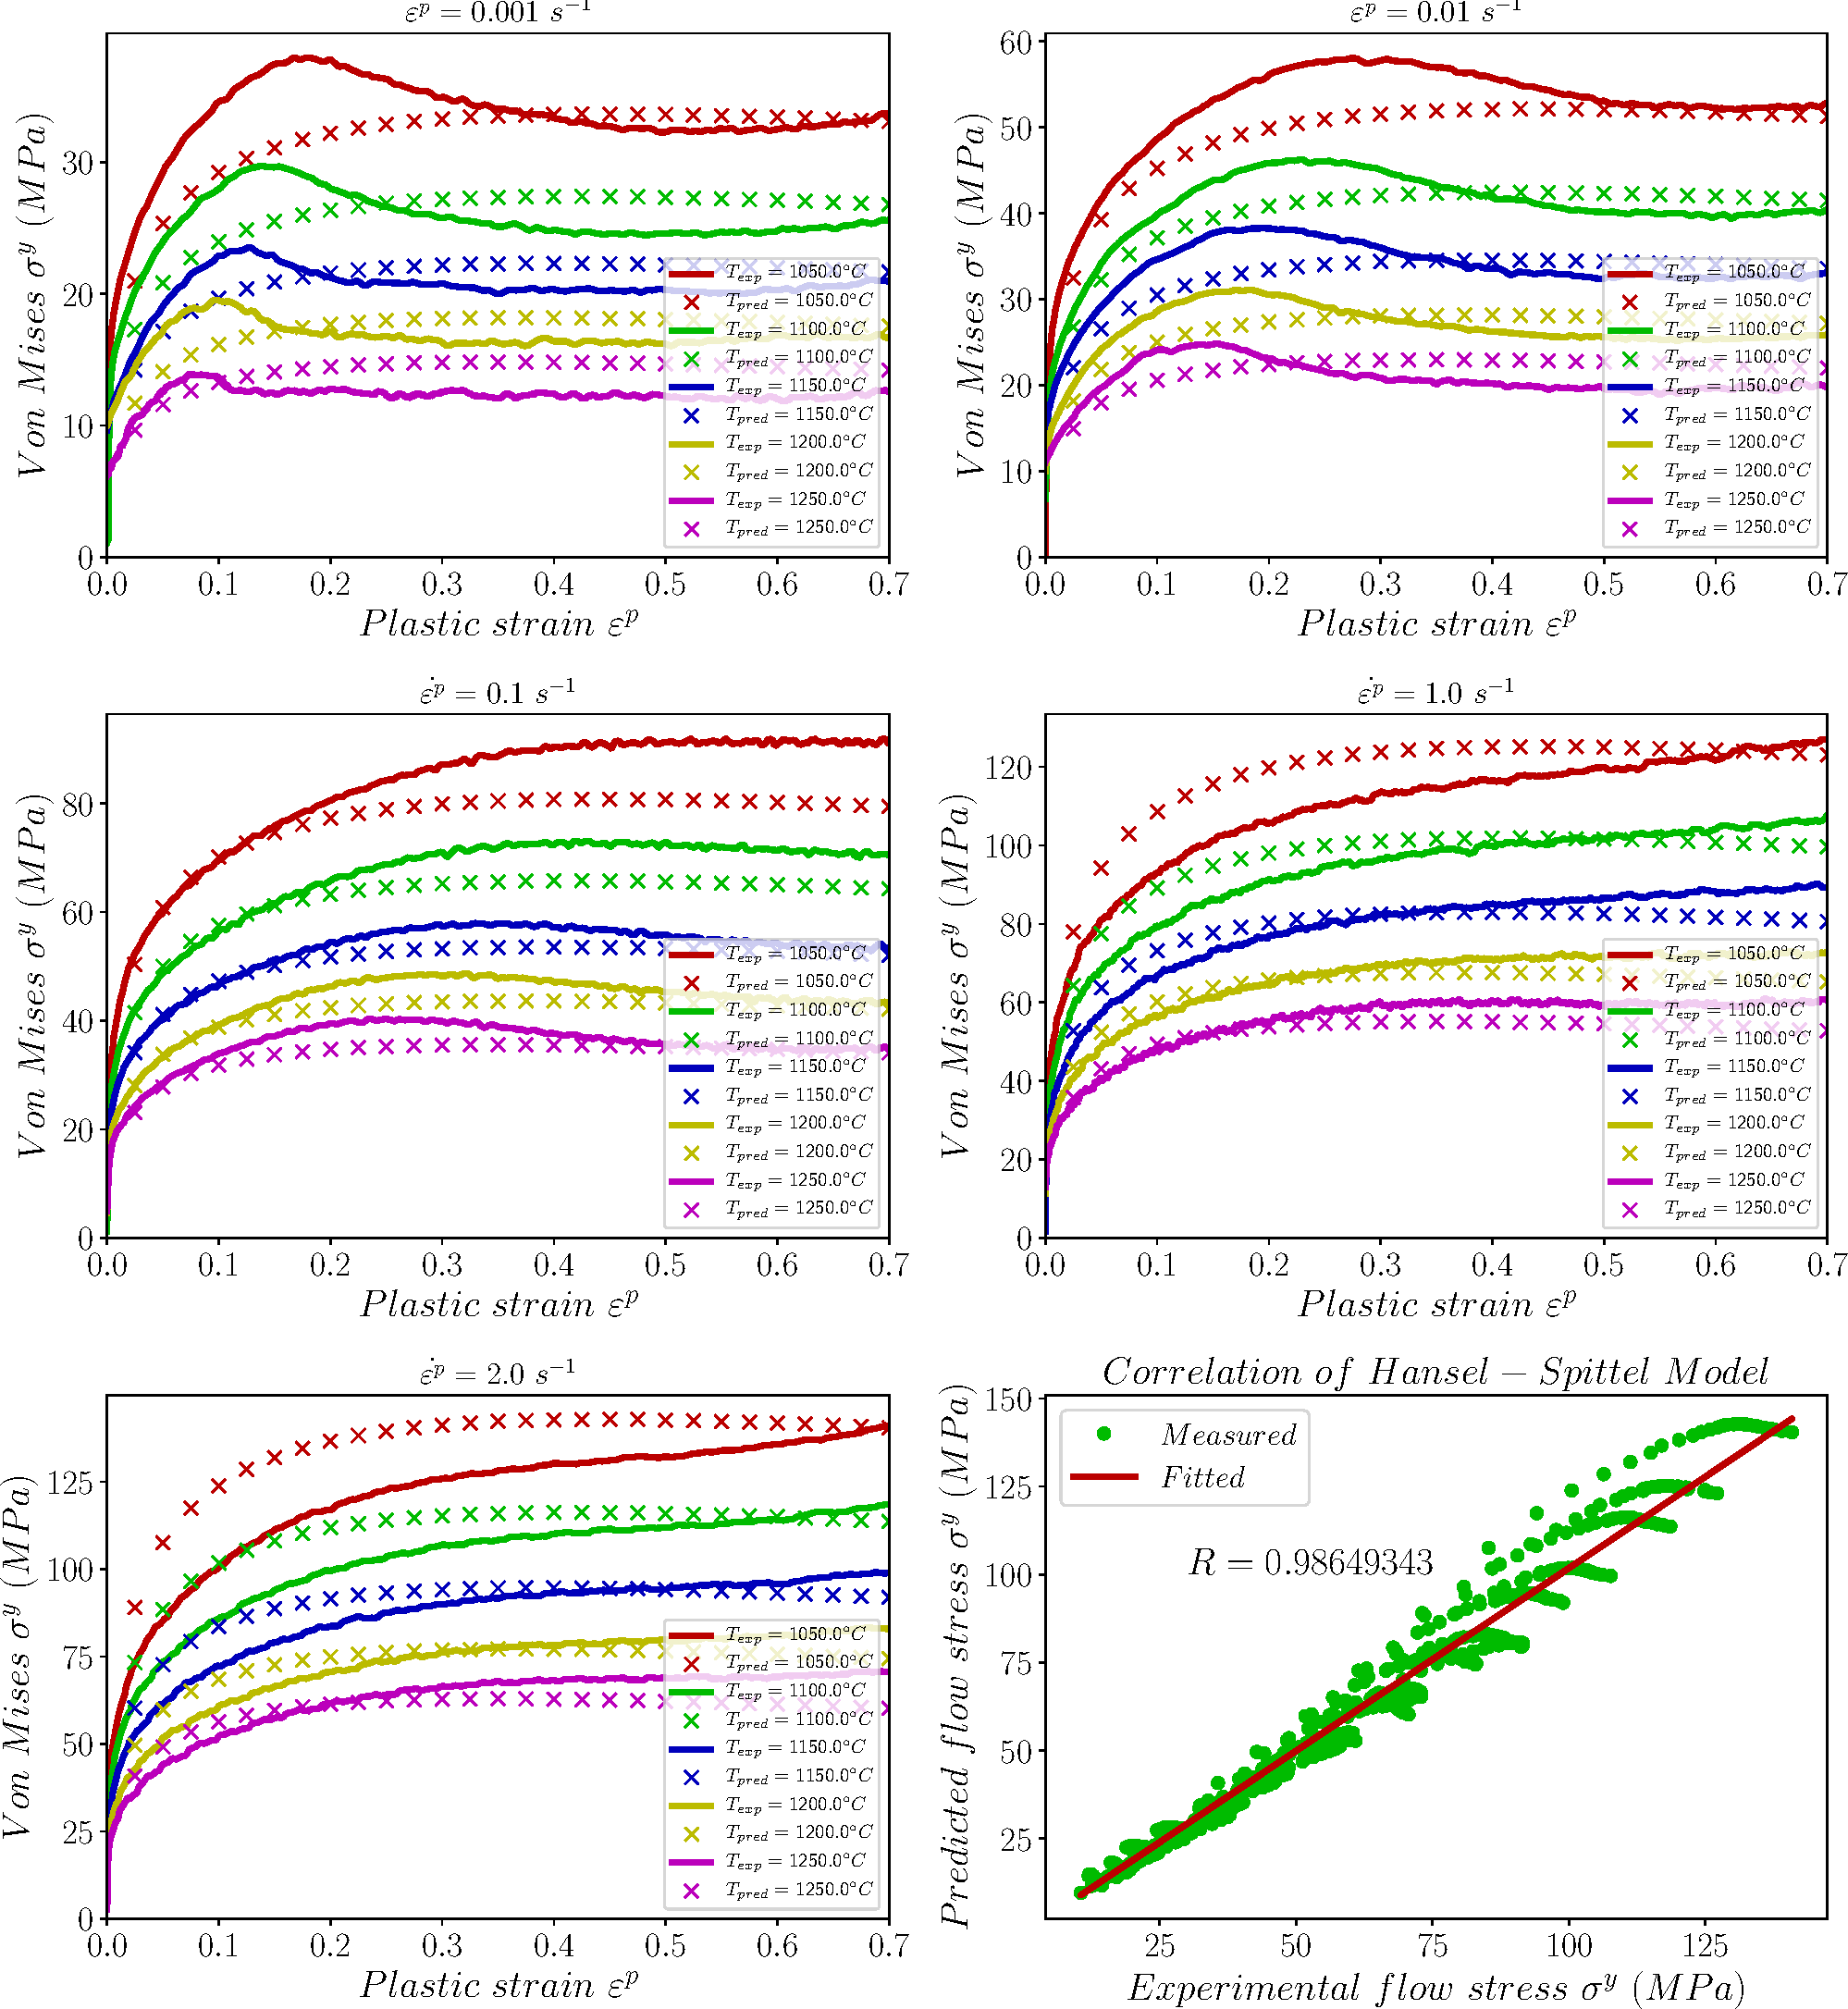
\includegraphics[width=1.02\columnwidth]
{newFigures/eCorrelationHS}
\caption{Comparison between the experimental and predicted flow stresses by HS model for extrapolation estimation}
\label{fig:eCorrelationHS}
\end{figure}
\FloatBarrier
%----------------------------------------------------------------------------------
\subsubsection{Arrhenius model (AR model), \label{sec:ARmodel}}
%----------------------------------------------------------------------------------
The Arrhenius tye model is one of the most widely used models, especially when it comes to studying the microstructure of the material. Indeed, this model takes into account the physical phenomena that describe the behaviour of the material and also the relations between stress ($\sigma^y$), strain ($\varepsilon^p$), the strain rate ($\mdot{\varepsilon}^p$) and the temperature ($T$) could be expressed in form of the power law, the exponential law and the hyperbolic sine type equation. This facilitates an easier description of the phenomenon of softening observed in material due to the increase in temperature. The following equations describe the Arrhenius model.
\begin{equation}
\label{eq:ARmodel1}
\mdot{\varepsilon}^p = A_1\sigma^{y^{n_1}}\exp\left(-\frac{Q}{RT}\right) \qquad (for ~~\alpha\sigma^y < 0.8)
\end{equation}
\begin{equation}
\label{eq:ARmodel2}
\mdot{\varepsilon}^p = A_2\exp(\beta\sigma^y)\exp\left(-\frac{Q}{RT}\right) \qquad (for ~~\alpha\sigma^y > 1.2)
\end{equation}
\begin{equation}
\label{eq:ARmodel}
\mdot{\varepsilon}^p = A_3\left[\sinh(\alpha\sigma^y)\right]^{n_2}\exp\left(-\frac{Q}{RT}\right) \qquad (for ~~all\ \sigma^y)
\end{equation}
Where $\mdot{\varepsilon}^p$ is the strain rate ($s^{-1}$), $Q$ is the deformation activation energy ($KJmol^{-1}$), $R$ is the universal gas constant ($8.314\ J mol^{-1} K^{-1}$), $T$ is the absolute temperature ($K$) and $A_1, A_2, A_3, n_1$, $n_2, \beta$ and $\alpha(\beta/n_1)$ are the material constants. To take into account the effects of temperature and strain rate on the deformation, a parameter ($Z$) called Zener--Hollomon parameter is introduced whose expression is given as follows:
\begin{equation}
\label{eq:Zparam}
Z = \mdot{\varepsilon}^p\exp\left(\frac{Q}{RT}\right)
\end{equation}
By replacing the relation (\ref{eq:ARmodel}) in the (\ref{eq:Zparam}) one it comes:
\begin{equation}
\label{eq:Zparam1}
Z = A_3\left[\sinh(\alpha\sigma^y)\right]^{n_2} \qquad \Rightarrow \qquad \sinh(\alpha\sigma^y) = \left(\frac{Z}{A_3}\right)^{1/n_2}
\end{equation}
Furthermore, it is known that:
\begin{equation}
arc\sinh(x) = \ln\left(x + \sqrt{1+x^2}\right)
\end{equation}
Therefore the Equation (\ref{eq:Zparam1}) becomes and which is actually the Arrhenius model: 
\begin{equation}
\sigma^y = \frac{1}{\alpha}\ln\left\{\left(\frac{Z}{A_3}\right)^{1/n_2} + \left[1 + \left(\frac{Z}{A_3}\right)^{2/n_2}\right]^{1/2}\right\}
\end{equation}
To obtain the constitutive equation, all parameters $\alpha$, $Q$, $n_2$, and $A_3$ needed to be determined. The following part shows the calculation procedures of these material constants at $0.1$ strain as example.\\
Taking the natural logarithm of Equations (\ref{eq:ARmodel1}) and (\ref{eq:ARmodel2}), the following relationships can be obtained: 
\begin{equation}
\ln \sigma^y = \frac{1}{n_1}\ln \mdot{\varepsilon}^p -\frac{1}{n_1}\ln A_1 +  \frac{1}{n_1}\frac{Q}{RT}
\end{equation}
\begin{equation}
\sigma^y = \frac{1}{\beta}\ln \mdot{\varepsilon}^p - \frac{1}{\beta}\ln A_2 + \frac{1}{\beta}\frac{Q}{RT} 
\end{equation}
From these two equations, we can easily deduce the parameters $n_1$ and $\beta$ as the slopes of the functions $\ln\sigma^y = f(\ln\mdot{\varepsilon}^p)$  and $\sigma^y = f(\ln\mdot{\varepsilon}^p)$ as shown in Figure \ref{fig:LnAlp} and Figure \ref{fig:LnSinhE0} for $0.1$ value of strain. It should be noted that later in this document all values of strain will be taken into account.
\begin{figure}[!ht]
\centering
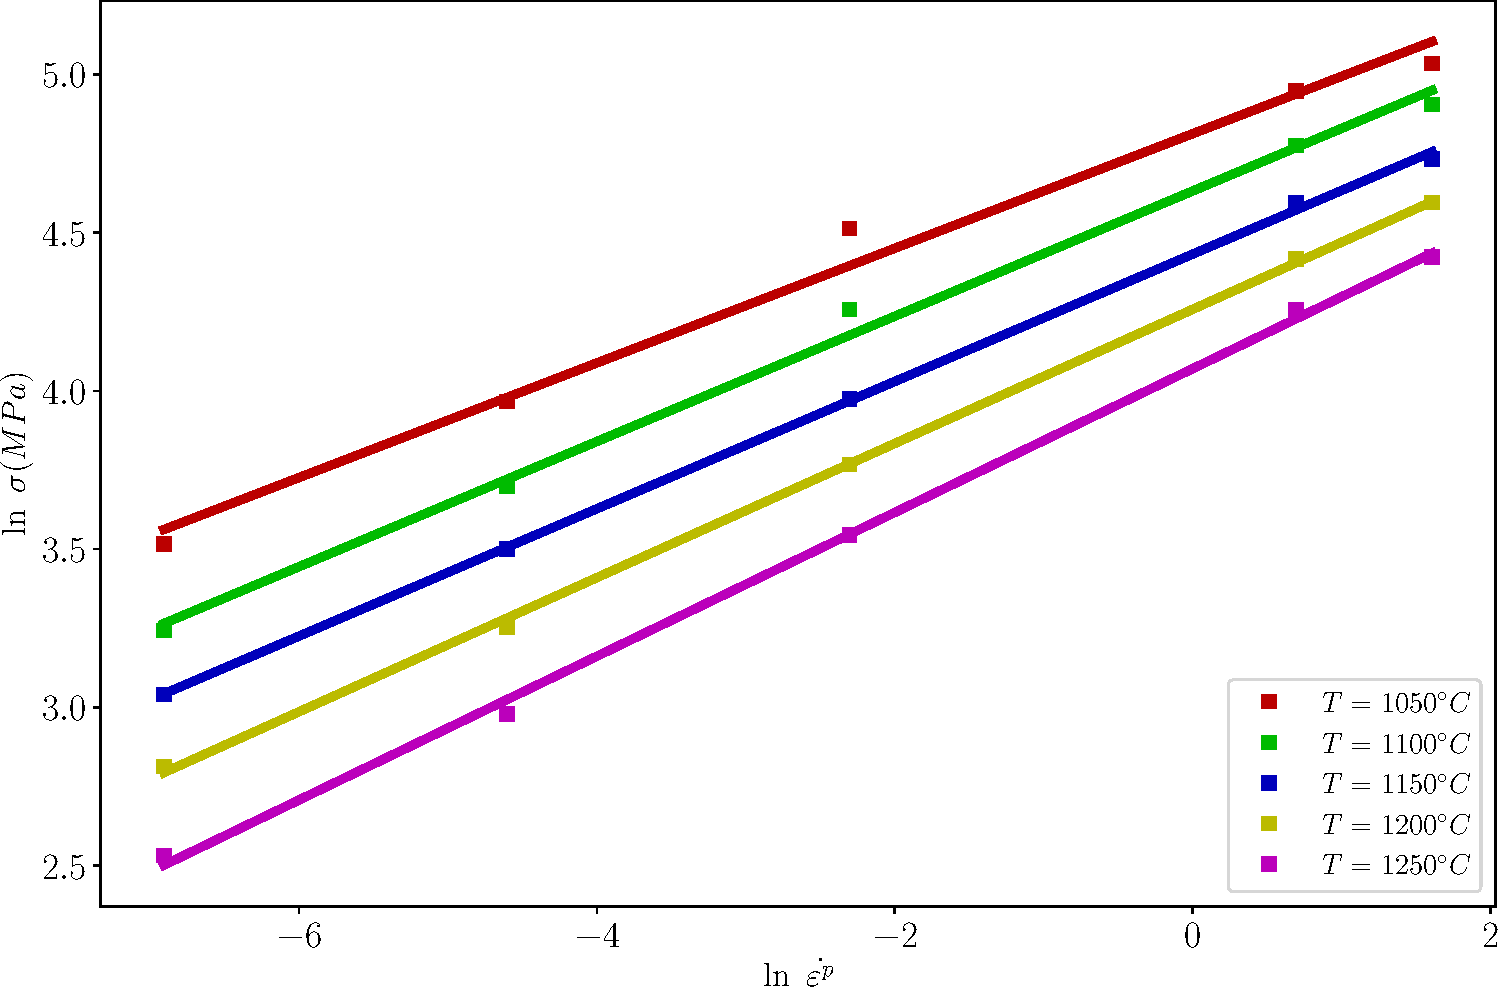
\includegraphics[width=0.9\columnwidth]{newFigures/LnAlp}
\caption{Relationship between $\ln \sigma^y$ and $\ln \dot{\varepsilon}^p$}
\label{fig:LnAlp}
\end{figure}
\begin{figure}[!ht]
\centering
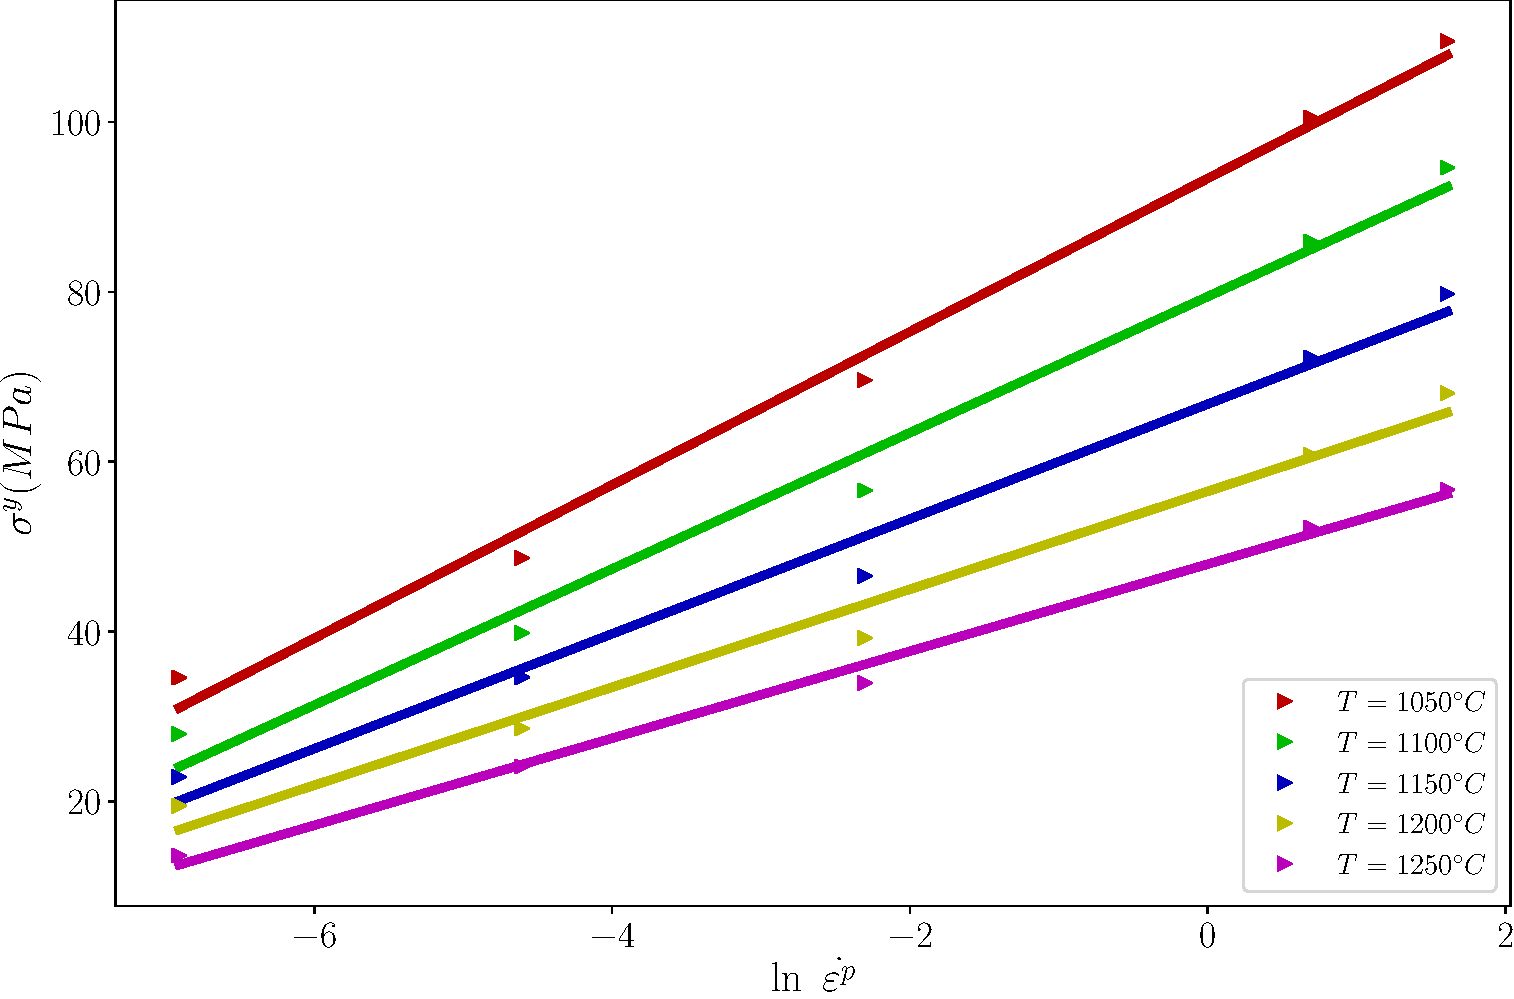
\includegraphics[width=0.9\columnwidth]{newFigures/LnSinhE0}
\caption{Relationship between $\sigma^y$ and $\ln \dot{\varepsilon}^p$}
\label{fig:LnSinhE0}
\end{figure}
The values of those parameters are therefore equal to $n_1=4.93599$ and $\beta=0.150438$ ($\alpha=\beta/n_1 = 0.0220306$). 
Taking the natural logarithm of Equation (\ref{eq:ARmodel}), the following relationship can be obtained:
\begin{equation}
\label{eq:lnSinh}
\ln\sinh(\alpha\sigma^y) = \frac{1}{n_2}\ln \mdot{\varepsilon}^p  -  \frac{1}{n_2}\ln A_3 + \frac{1}{n_2} \frac{Q}{RT}
\end{equation}
By applying the chain derivative rule, we get the following relationship to calculate the energy activation coefficient $Q$.
\begin{equation}
\label{eq:parQ}
Q = R\left[\frac{\partial \ln \mdot{\varepsilon}^p}{\partial \ln [\sinh(\alpha\sigma^y)]}\right]_{T}\left[\frac{\partial \ln [\sinh(\alpha\sigma^y)]}{\partial (1/T)}\right]_{\mdot{\varepsilon}^p}= Rn_2\frac{d\left\{\ln\left[\sinh(\alpha\sigma^y)\right]\right\}}{d(1/T)}
\end{equation}
From Equation (\ref{eq:lnSinh}) and Equation (\ref{eq:parQ}) we can deduce the parameters $n_2 $ and $Q $ from the slopes of the functions $\ln \sinh(\alpha\sigma^y) = f(\ln \dot{\varepsilon}^p)$ and $\ln \sinh(\alpha\sigma^y) = g(1/T)$ as shown in Figure \ref{fig:LnSinhE} and Figure \ref{fig:LnSinhT}. Thus those values are $3.21374$ and $432.722\ KJ.mol^{-1}$ respectively.
\begin{figure}[!ht]
\centering
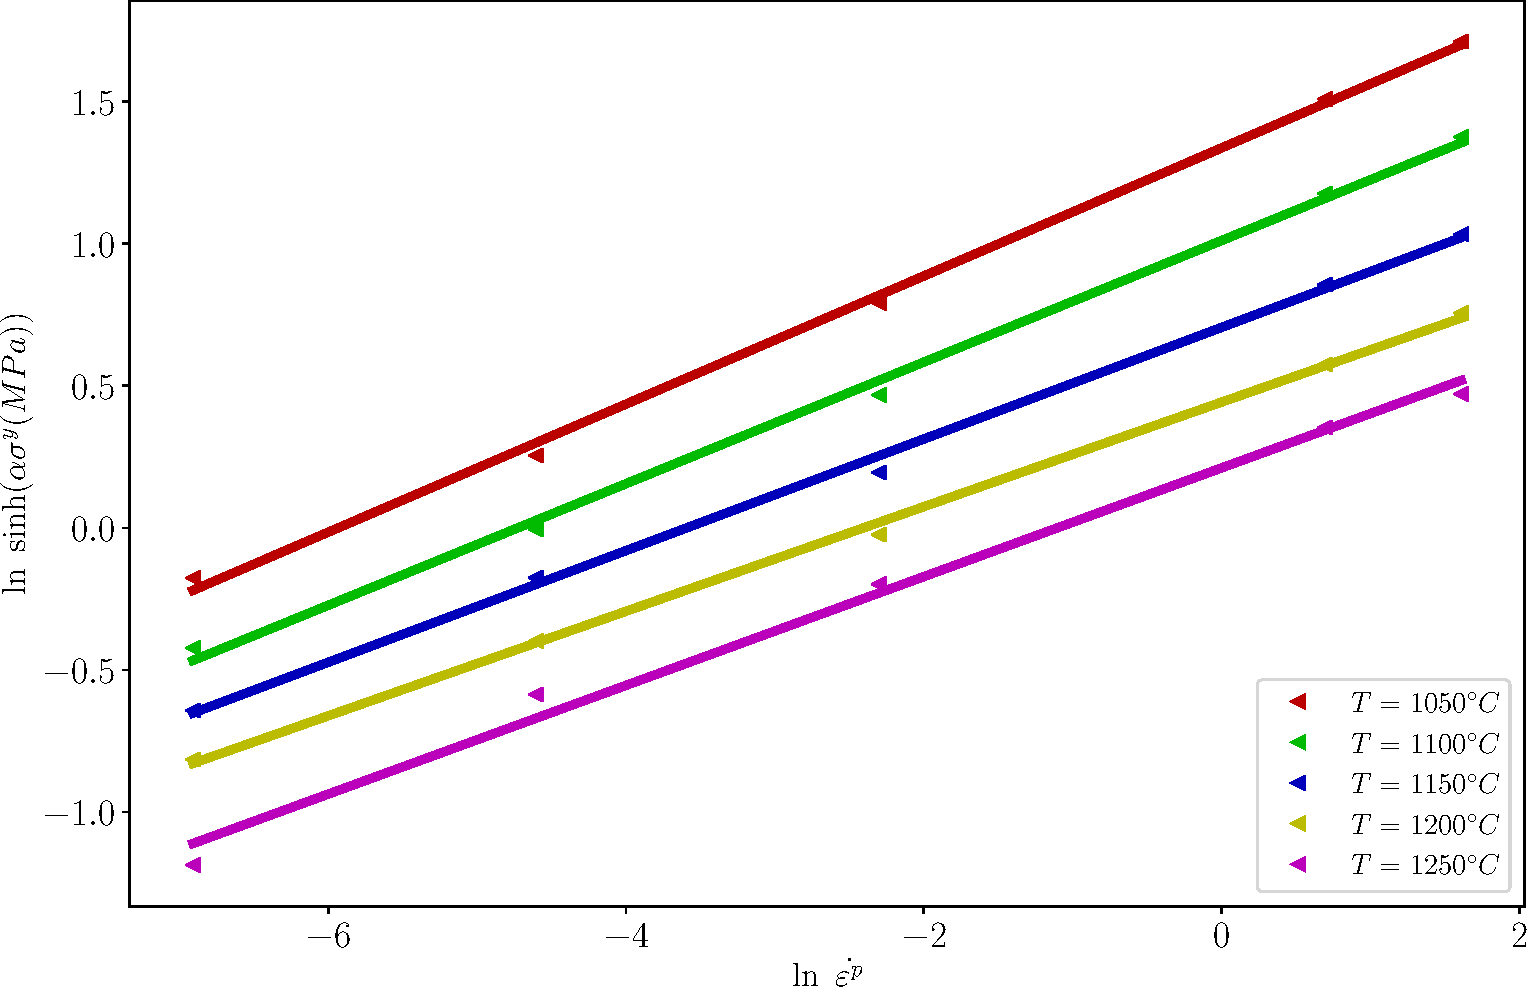
\includegraphics[width=0.9\columnwidth]{newFigures/LnSinhE}
\caption{Relationship between $\ln \sinh(\alpha\sigma^y) $ and $\ln \dot{\varepsilon}^p$}
\label{fig:LnSinhE}
\end{figure}
\begin{figure}[!ht]
\centering
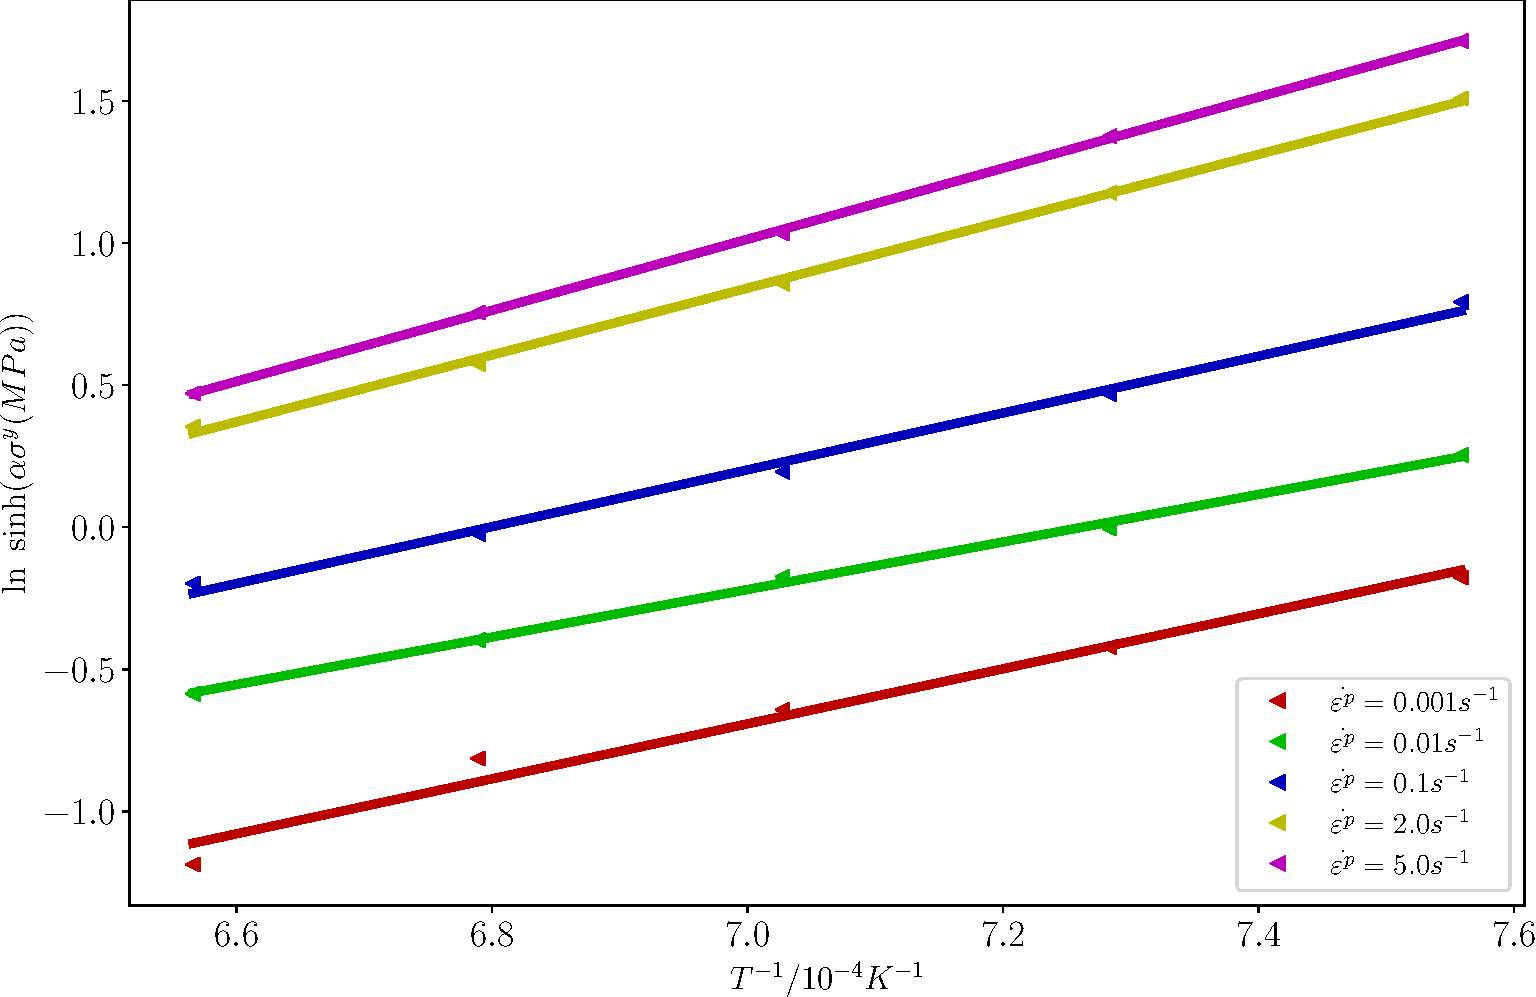
\includegraphics[width=0.9\columnwidth]{newFigures/LnSinhT}
\caption{Relationship between $\ln \sinh(\alpha\sigma^y) $ and $1/T$}
\label{fig:LnSinhT}
\end{figure}
As these coefficients are calculated for a single strain value as example, it is possible to take into account their dependence on all strain values. Hence the need to find a function for each coefficient for all temperatures and strains. Figure  \ref{fig:ARparameters} shows the relationships between $\alpha$, $Q$, $n$, $\ln A$ and true strain $\varepsilon^p$ for P20 alloy using leasquare method to fit the measured data. For each parameter (whose strain dependant expressions are given by Equations \ref{eq:alpha}, \ref{eq:Q}, \ref{eq:n} and \ref{eq:lnA}), the values of constants are summarized in Table \ref{tab: ARparameters}. Figure \ref{fig:iCorrelationAR} and Figure\ref{fig:eCorrelationAR} are the comparison of predicted values of AR model and experimental values where the correlaton is good. The gap between experimental and prediction is small. But for the strain rate $\mdot{\varepsilon}^p = 0.01$ and for the two low temperatures values, the AR model is not able to predict the softening.
\begin{equation}
\label{eq:alpha}
\alpha(\varepsilon^p) = \alpha_0 + \alpha_1\varepsilon^{{p^1}} + \alpha_2\varepsilon^{p^2} + \alpha_3\varepsilon^{p^3} + \alpha_4\varepsilon^{p^4} + \alpha_5\varepsilon^{p^5} + \alpha_6\varepsilon^{p^6}
\end{equation}
\begin{equation}
\label{eq:Q}
Q(\varepsilon^p) = Q_0 + Q_1\varepsilon^{{p^1}} + Q_2\varepsilon^{p^2} + Q_3\varepsilon^{p^3} + Q_4\varepsilon^{p^4} + Q_5\varepsilon^{p^5} + Q_6\varepsilon^{p^6}
\end{equation}
\begin{equation}
\label{eq:n}
n(\varepsilon^p) = n_0 + n_1\varepsilon^{{p^1}} + n_2\varepsilon^{p^2} + n_3\varepsilon^{p^3} + n_4\varepsilon^{p^4} + n_5\varepsilon^{p^5} + n_6\varepsilon^{p^6}
\end{equation}
\begin{equation}
\label{eq:lnA}
\ln A(\varepsilon^p) = \ln A_0 + \ln A_1\varepsilon^{{p^1}} + \ln A_2\varepsilon^{p^2} + \ln A_3\varepsilon^{p^3} + \ln A_4\varepsilon^{p^4} + \ln A_5\varepsilon^{p^5} + \ln A_6\varepsilon^{p^6}
\end{equation}
\begin{figure}[!ht]
\centering
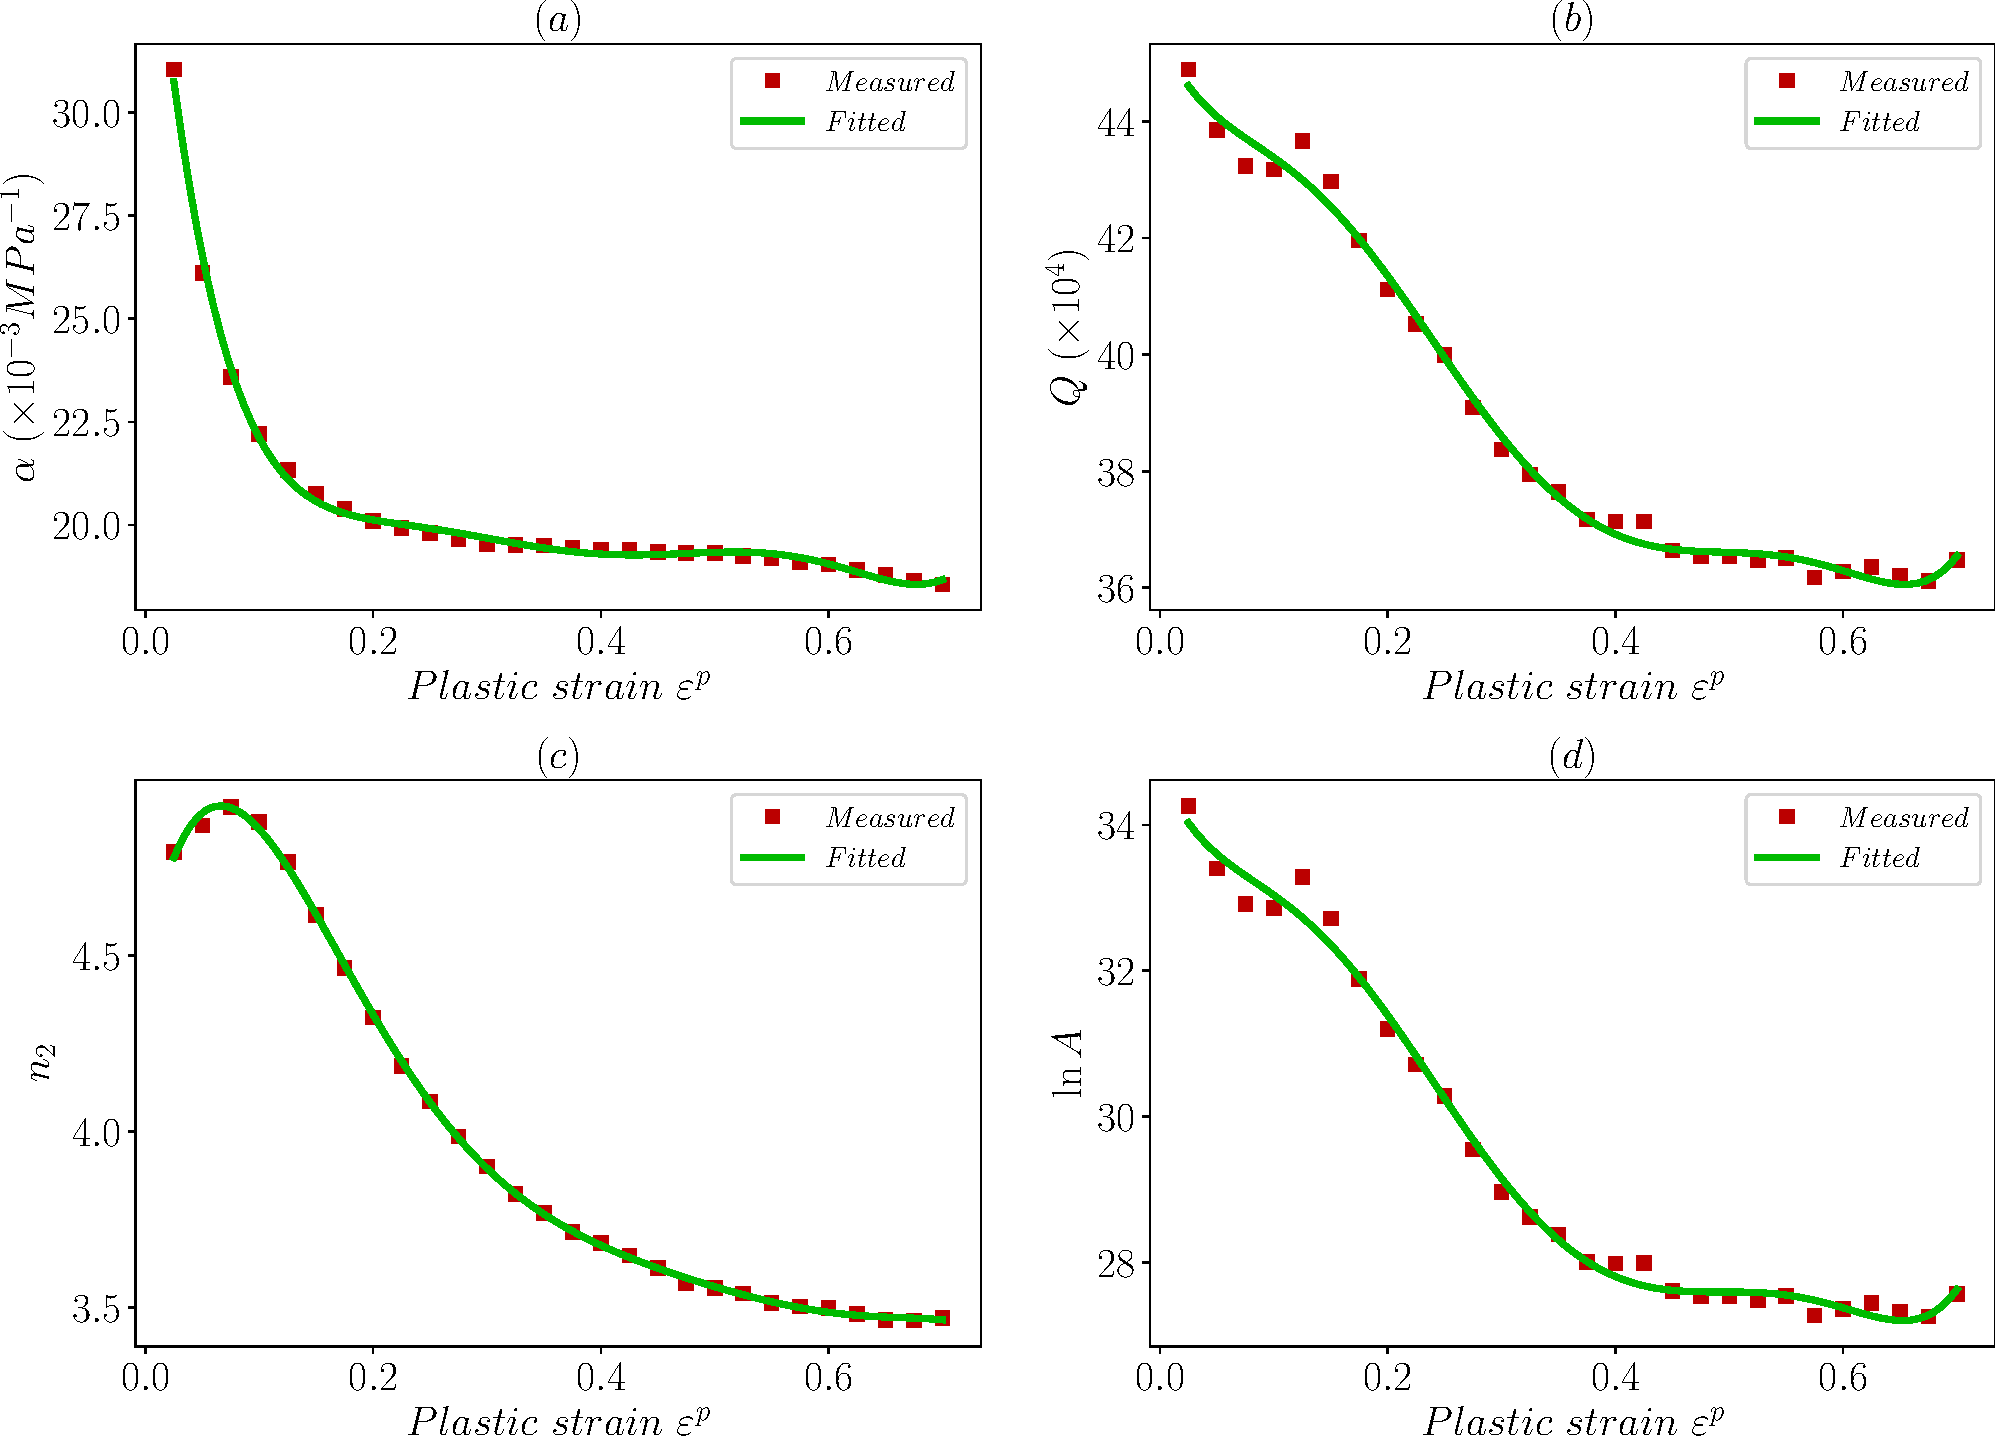
\includegraphics[width=1.02\columnwidth]{newFigures/ARparameters}
\caption{Relationships between $\alpha$ (a)  , $Q$ (b) , $n$ (c)  and $lnA$ (d)  with the true strain $\varepsilon^p$ by polynomial functions}
\label{fig:ARparameters}
\end{figure}
\begin{table}[h!]
\centering{}
\caption{Parameters' constants of Arrhenius Model}
\scalebox{0.95}{
\begin{tabular}{lllll}
\hline
&						&				   &				  &\\
&$\alpha$          & $Q (\times10^{6})$ & $n$      & $\ln A$\\
&						&				   &				  &\\
\hline
&$\alpha_0 = 0.0368199$ & $Q_0 = 0.451215$  & $n_0 = 4.52844$ & $\ln A_0 = 34.4714$\\
&$\alpha_1 = -0.300454$ & $Q_1 = -0.526197$ & $n_1 = 15.6433$ & $\ln A_1 = -42.818$\\
&$\alpha_2 = 2.19468$   & $Q_2 =5.99635 $ & $n_2 = -176.65$ & $\ln A_2 = 493.325$\\
Interpolation&$\alpha_3 =-8.29695$ & $Q_3 =-37.4915 $  & $n_3 = 682.187$ & $\ln A_3 =-3095.19 $\\
&$\alpha_4 = 16.8067$   & $Q_4 = 102.928$  & $n_4 = -1289.52$& $\ln A_4 = 8516.02$\\
&$\alpha_5 = -17.2641$  & $Q_5 =-127.865$  & $n_5 = 1205.95$ & $\ln A_5 = -10594.8$\\
&$\alpha_6 = 7.04353$   & $Q_6 = 59.2928$  & $n_6 =-446.166$ & $\ln A_6 = 4918.17$\\
%\hdashline
&$\alpha_0 = 0.0392338$ & $Q_0 = 0.437281$  & $n_0 = 4.3178$ & $\ln A_0 = 32.872$\\
&$\alpha_1 =-0.323238$ & $Q_1 =-0.401528$ & $n_1 = 17.3196$ & $\ln A_1 = -32.2877$\\
&$\alpha_2 = 2.38426$   & $Q_2 = 4.86745$ & $n_2 = -192.485$ & $\ln A_2 = 397.553$\\
Extrapolation&$\alpha_3 = -9.04342$& $Q_3 = -33.2061$& $n_3 = 752.451$ & $\ln A_3 =-2725.91 $\\
&$\alpha_4 = 18.34$   & $Q_4 = 95.0889$  & $n_4 = -1450.86$& $\ln A_4 = 7825.29$\\
&$\alpha_5 = -18.8254$  & $Q_5 =-120.398$  & $n_5 = 1391.74$ & $\ln A_5 =-9924.46$\\
&$\alpha_6 = 7.66332$   & $Q_6 = 56.2666$  & $n_6 =-530.417$ & $\ln A_6 = 4644.18$\\
\hline
\label{tab: ARparameters}
\end{tabular}}
\end{table}
\begin{figure}[!ht]
\centering
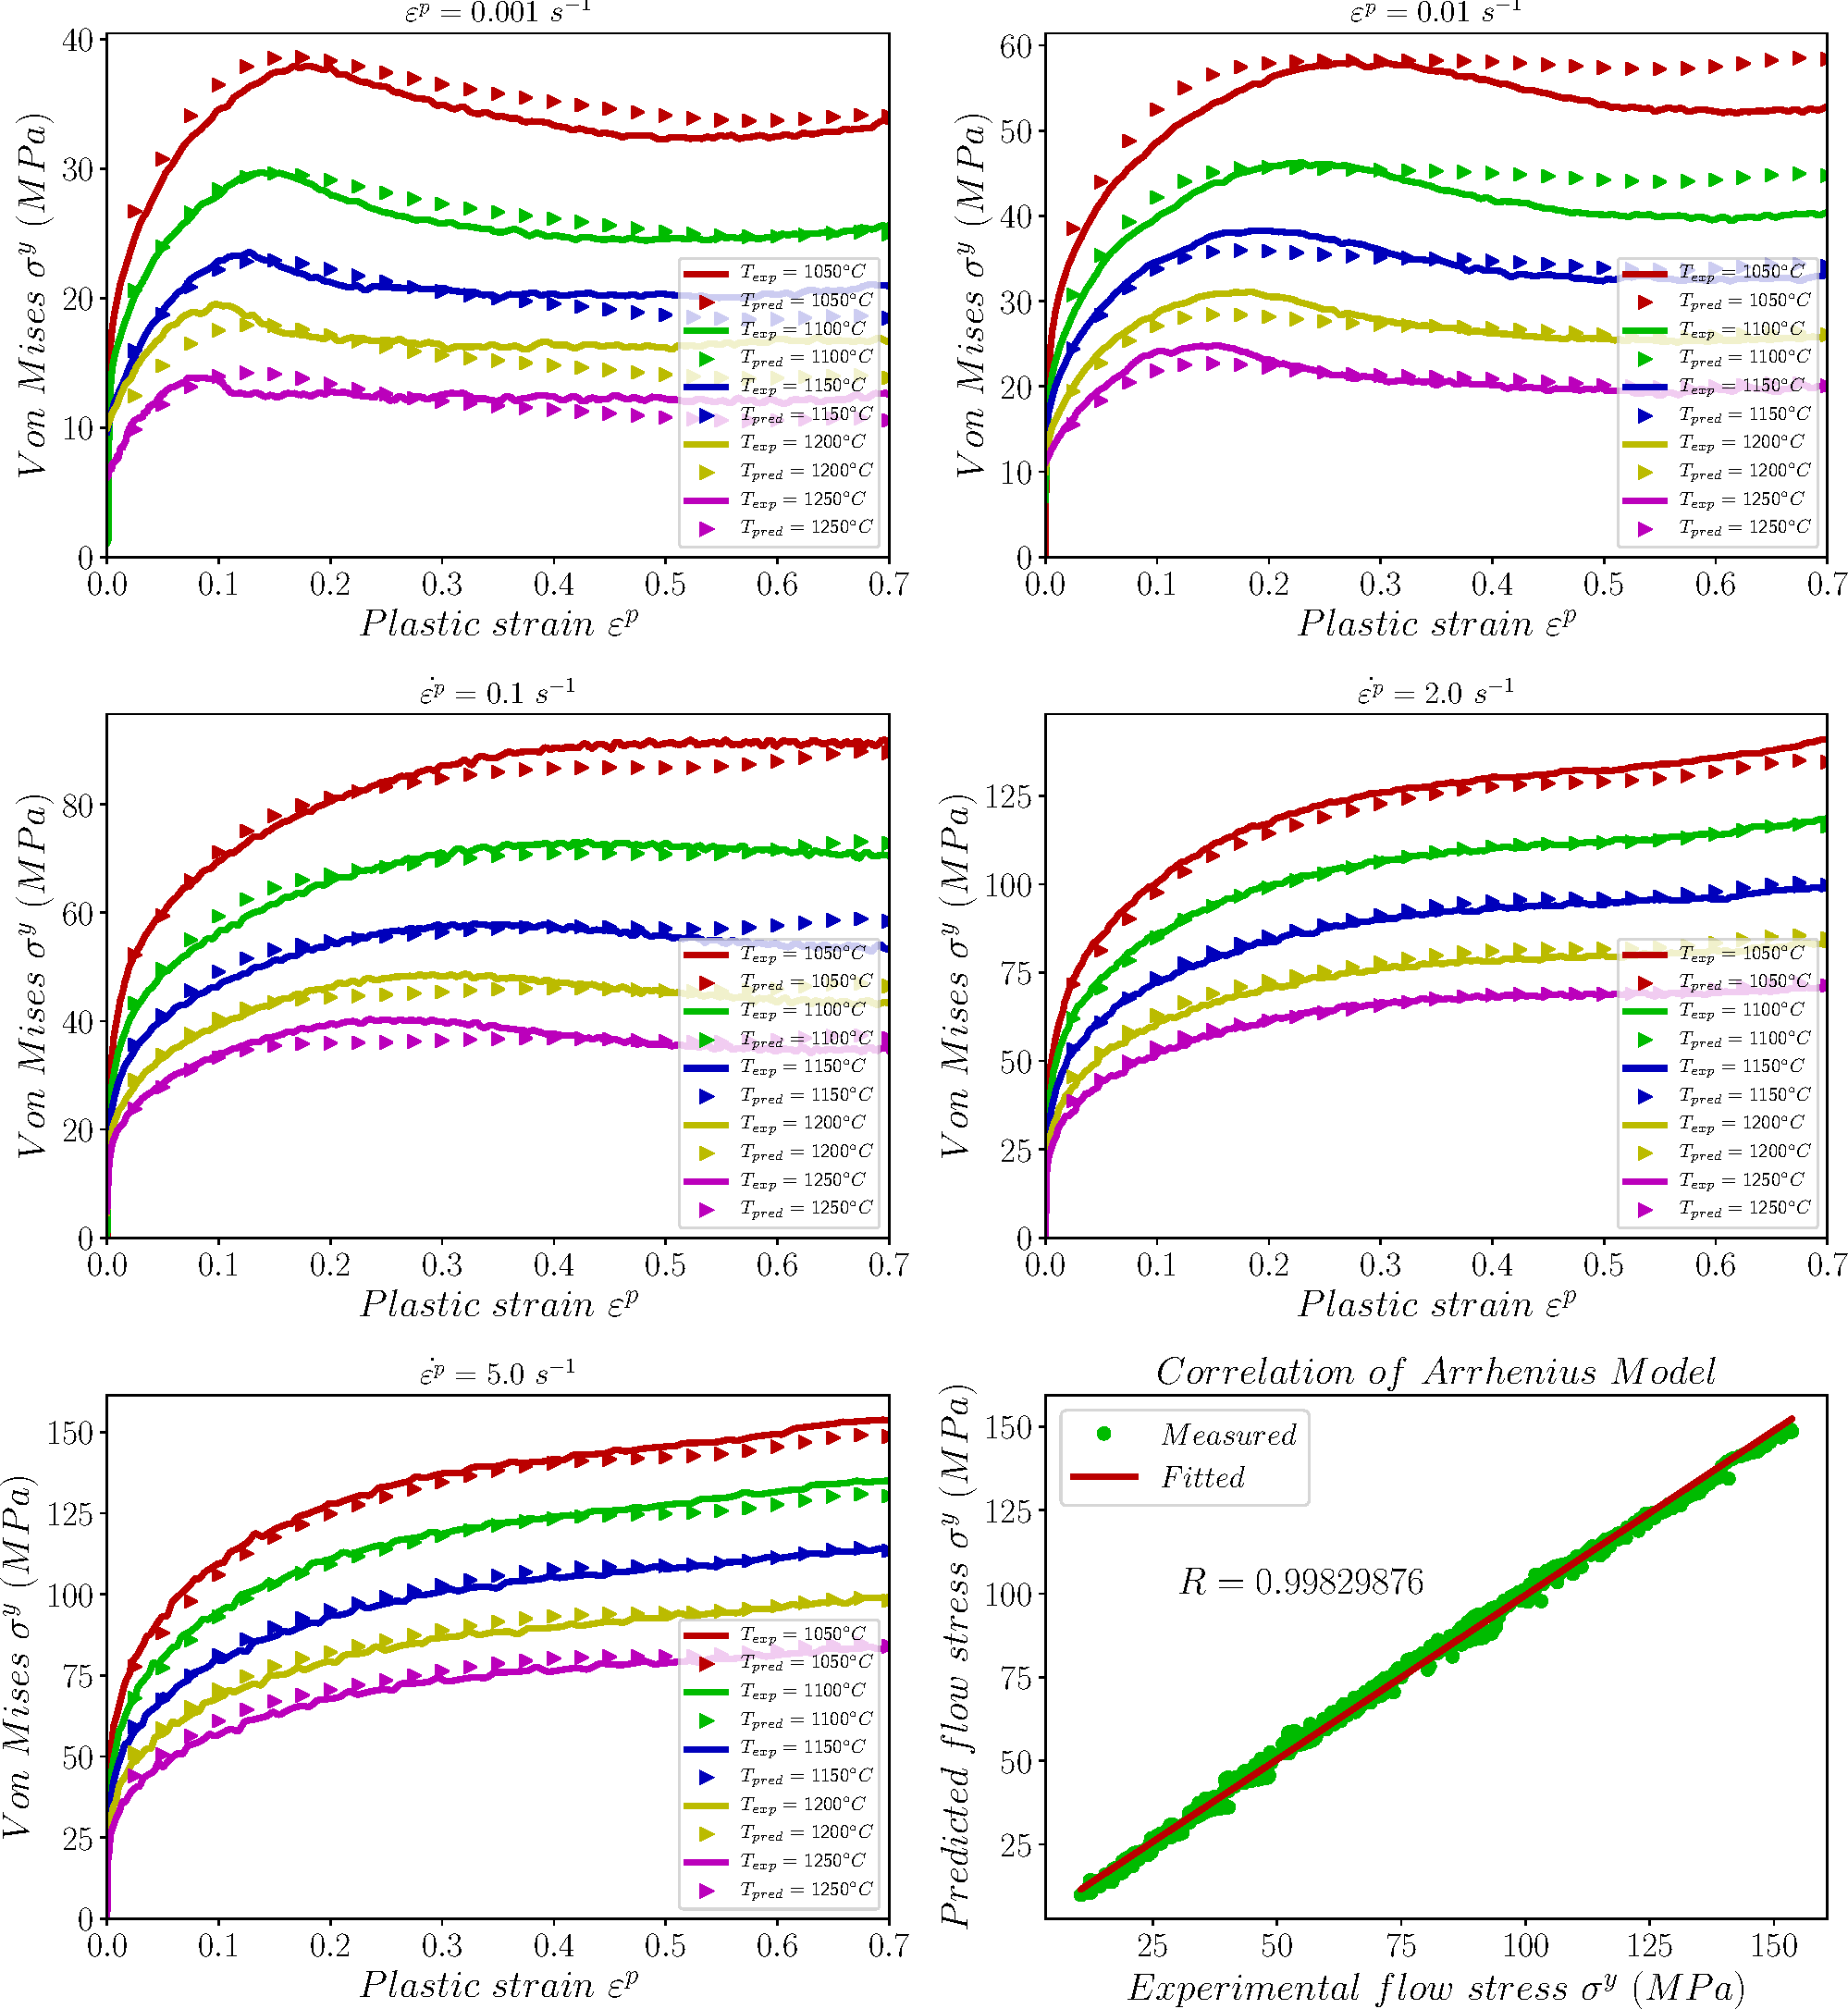
\includegraphics[width=1.02\columnwidth]
{newFigures/iCorrelationAR}
\caption{Comparison between the experimental and predicted flow stresses by AR model for interpolation estimation}
\label{fig:iCorrelationAR}
\end{figure}
\begin{figure}[!ht]
\centering
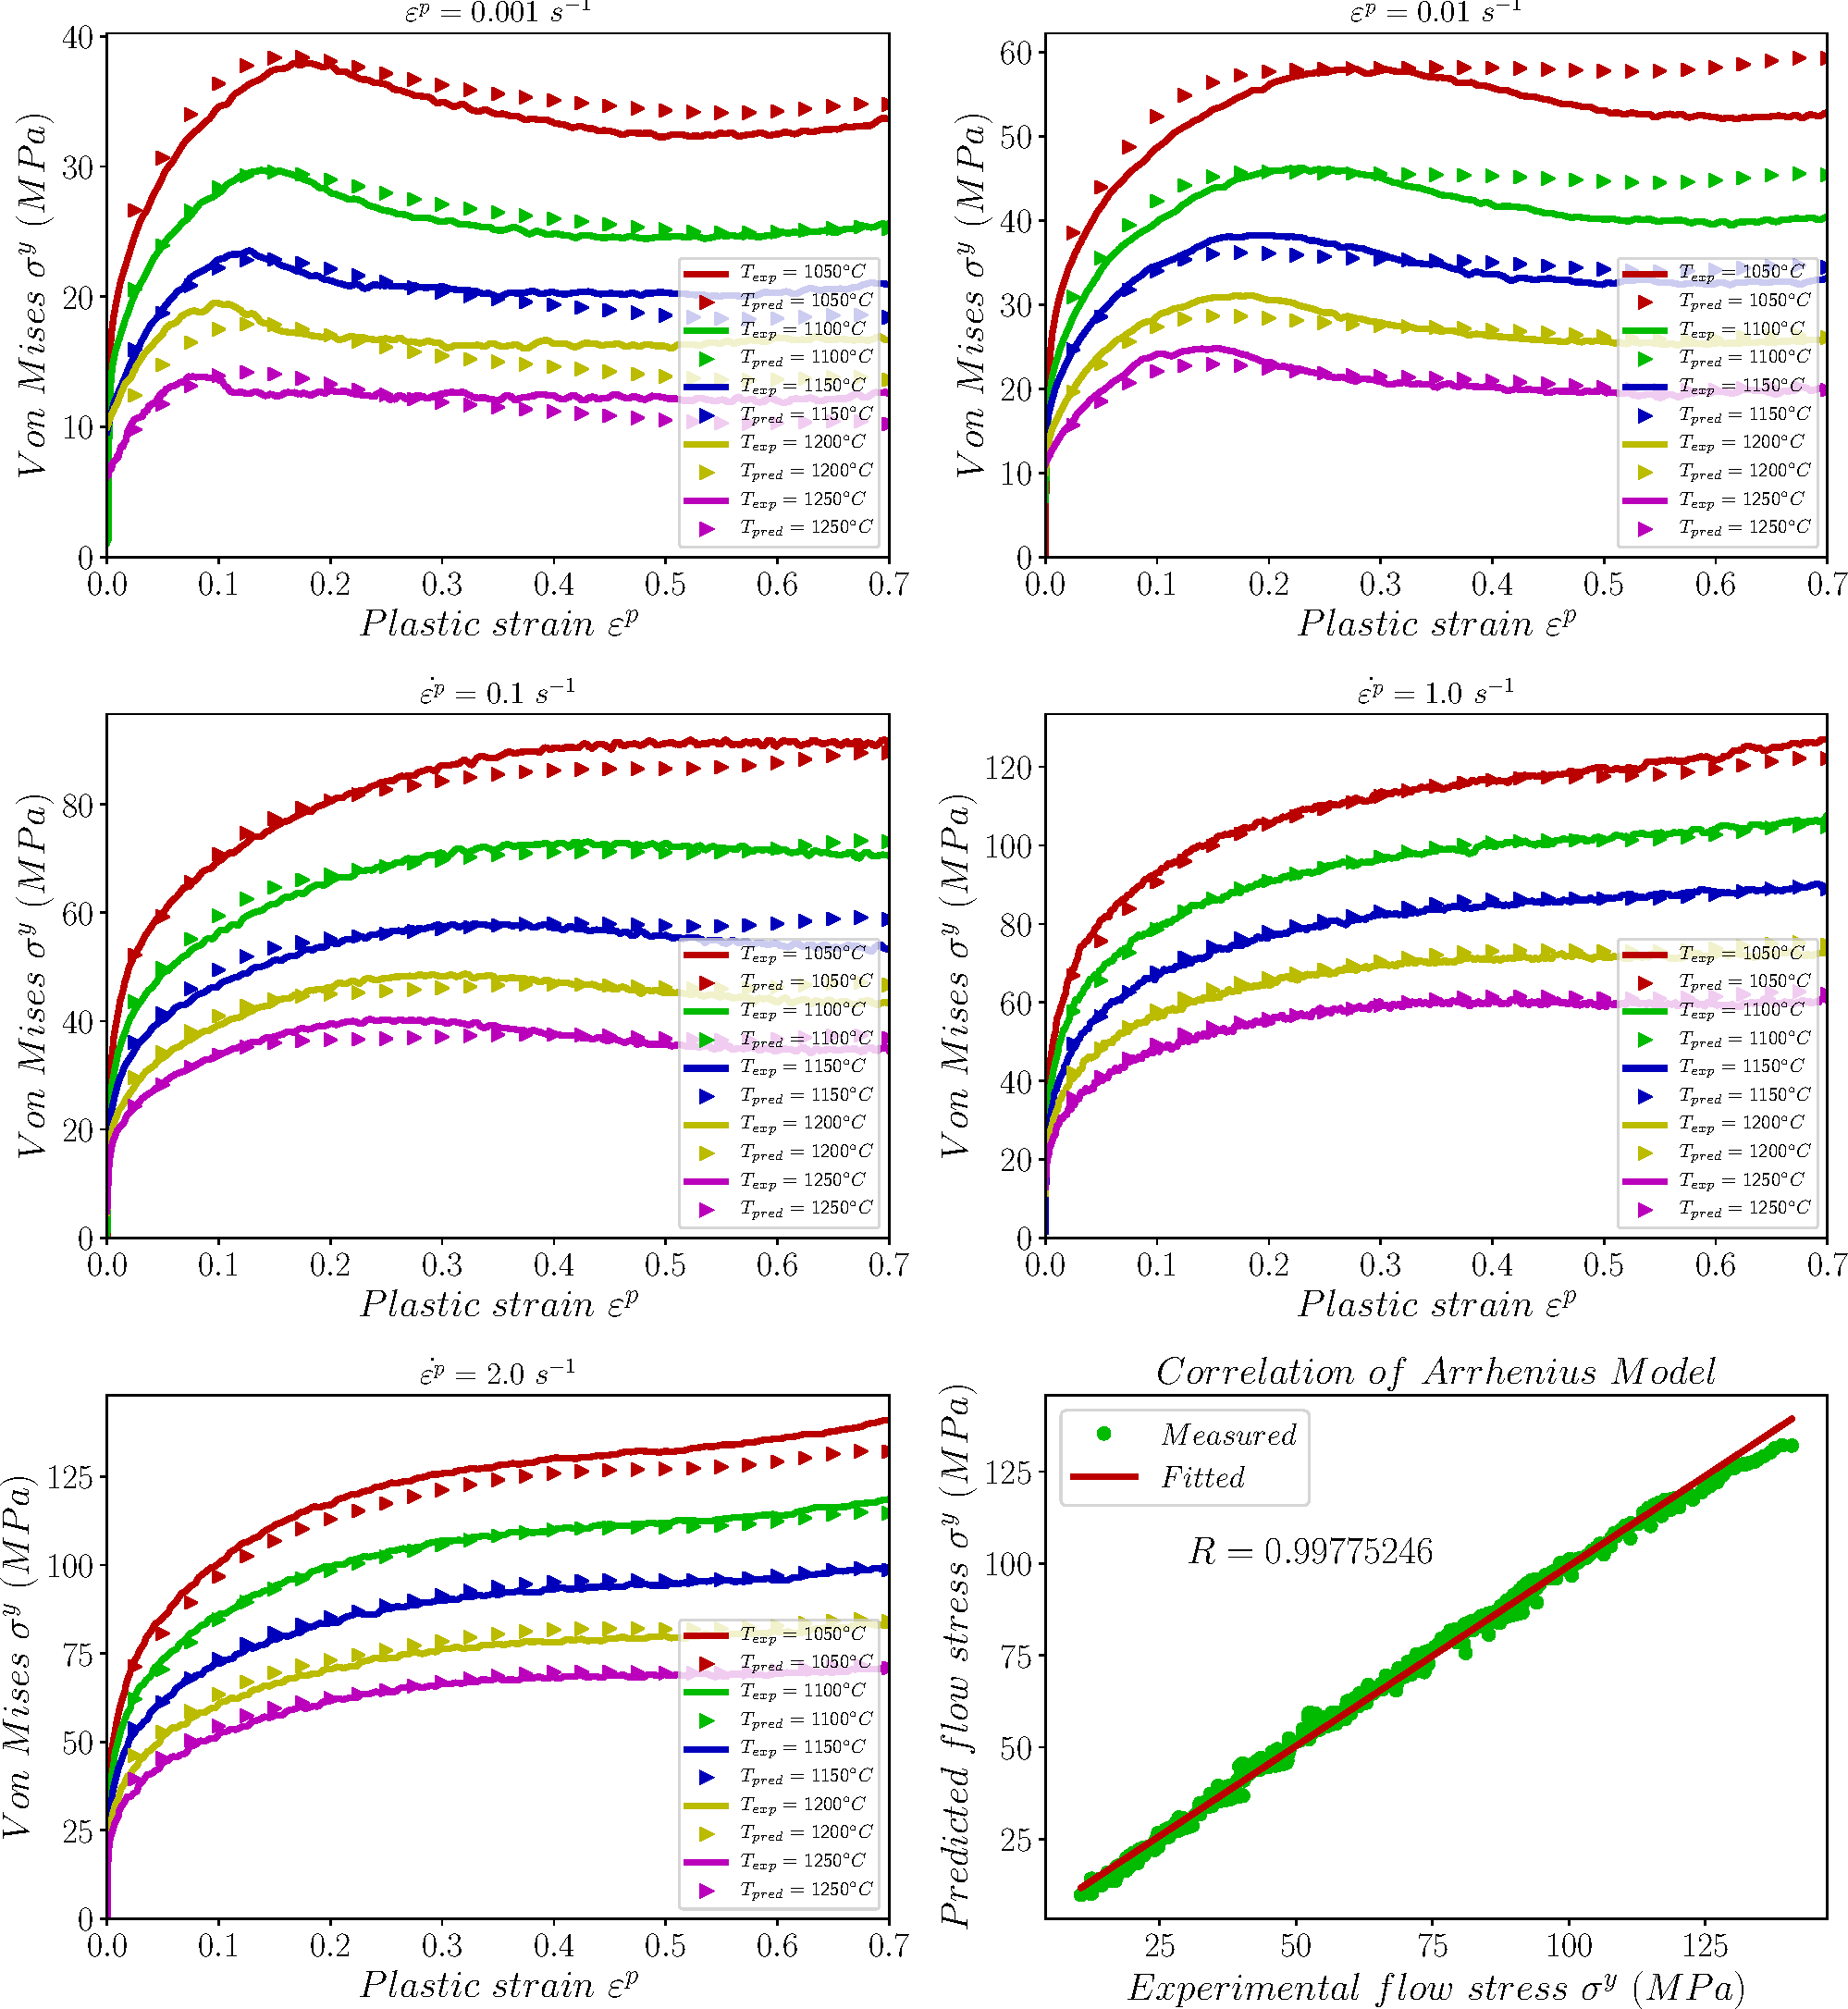
\includegraphics[width=1.02\columnwidth]
{newFigures/eCorrelationAR}
\caption{Comparison between the experimental and predicted flow stresses by AR model for extrapolation estimation}
\label{fig:eCorrelationAR}
\end{figure}
\FloatBarrier
%-------------------------------------------------------------------------
\subsubsection{Proposed model (PTM model)\label{sec:ProposedModel}}
%--------------------------------------------------------------------------
The PTM model is a generalized formulation of the MZA model. Indeed, the shortcomings of the MZA model are taken into account in this formulation, which makes the model flexible for any type of studied material as it does not require a limited number of parameters. The intrinsic functions of the model, which are the polynomial type functions, will determine the parameters of the model according to the degree of the polynomial, which provides a good fit for each function. The direct objective of this work being to demonstrate the ability of the neural network based model to override analytical models in the term of interpolation and extrapolation, it is important to point out that the PTM model can give better results than those presented in this work. For more details of this model we invite the reader to consult our previous work \cite{tize2022generalized}. The equation describing the PTM model is therefore given by:
\begin{equation}
\label{eq:PTM-model}
\sigma^y(\varepsilon^p,\mdot{\varepsilon}^p,T) = \left(\sum_{i=0}^{q}{A_i\varepsilon^{p^i}}\right) \exp\left[\left(\sum_{j=0}^{r}{B_j\varepsilon^{p^j}}\right)\left(T-T_0\right) + \left(\sum_{k=0}^{s}\left(\sum_{l=0}^{t}{C_k^l\varepsilon^{p^l}} \right)\left(T-T_0\right)^k \right)\ln\left( \frac{\mdot{\varepsilon}^p}{\mdot{\varepsilon}_0}\right)\right]
\end{equation}
where $A_i, B_j, C_k^l$ are the parameters of the model to be identified using the procedure proposed in  \cite{tize2022generalized}. Quantities $q$, $r$, $s$ and $t$ define the degree of the polynomials used to describe the behavior of the material. The larger these quantities are, the more parameters need to be identified for the PTM model.

The determination of the parameters of this model are calculated thanks to the LMFIT Python library \cite{Newville-2016-LNL} and according to the following three steps:
\begin{itemize}
\item \textbf{Step 1} : Determination of the two functions $I_1(\varepsilon^p)$ and $S_1(\varepsilon^p)$\\
At the reference strain rate, \ie when $\mdot{\varepsilon}^p=\mdot{\varepsilon}_0$, Equation (\ref{eq:PTM-model}) is written as:
\begin{equation}
\sigma^y(\varepsilon^p,T) = \left(\sum_{i=0}^{q}{A_i\varepsilon^{p^i}}\right)
\exp\left[\left(\sum_{j=0}^{r}{B_j\varepsilon^{p^j}}\right)\left(T-T_0\right) \right]
\end{equation}
Taking the logarithm of each member of this equation we obtain:
\begin{equation}
\label{eq:I1S0}
\ln \sigma^y(\varepsilon^p,T) = I_1(\varepsilon^p) + S_1(\varepsilon^p)\left(T-T_0\right)
\end{equation}
where:
\begin{equation}
\label{eq:I1S1}
I_1(\varepsilon^p) = \ln\left(\sum_{i=0}^{q}{A_i\varepsilon^{p^i}}\right)\qquad \text{and}\qquad S_1(\varepsilon^p) = \sum_{j=0}^{r}{B_j\varepsilon^{p^j}}
\end{equation}
Plotting the function $\ln \sigma^y(T)$ for a given value of $\varepsilon^p$ allows us to deduce $I_1(\varepsilon^p)$ and $S_1(\varepsilon^p)$ from the y-intercept and the slope, respectively. These functions are calculated for all plastic strain values $\varepsilon^p$ available in the experimental database. Analysis of those results allows us to propose some adequate values for the $q$ and $r$ quantities. Once those values have been selected, an identification procedure allow us to compute the $q$ parameters $A_i$ and $r$ parameters $B_j$ of the PTM model.
\item \textbf{Step 2} : Determination of the function $S_2(\varepsilon^p,T)$ as polynomials depending on the temperature $T$\\
Once the Step $1$ is done, it is possible to take the logarithm of the whole Equation (\ref{eq:PTM-model}) to obtain:
\begin{equation}
\ln \sigma^y(\varepsilon^p,\mdot{\varepsilon}^p,T) - I_1(\varepsilon^p) - S_1(\varepsilon^p)\left(T-T_0\right) = S_2(\varepsilon^p,T)\ln\left( \frac{\mdot{\varepsilon}^p}{\mdot{\varepsilon}_0}\right)
\label{eq:SlopeS2}
\end{equation}
where :
\begin{equation}
S_2 (\varepsilon^p,T)= \sum_{k=0}^{s}\left(\sum_{l=0}^{t}{C_k^l\varepsilon^{p^l}} \right)\left(T-T_0\right)^k
\label{eq:S2_coefs}
\end{equation}
From this latter the plot of $\ln \sigma^y - I_1(\varepsilon^p) - S_1(\varepsilon^p)\left(T-T_0\right)$ versus $\ln(\mdot{\varepsilon}^p/\mdot{\varepsilon}_0)$ allows us to deduce $S_2(\varepsilon^p,T)$ as its slope for a given plastic strain value $\varepsilon^p$. The evolution of $S_2$ versus $\left(T-T_0\right)$ allows to find the same function for all plastic strains which is described in the polynomial forms of degree $k$ in Equation (\ref{eq:PTM-model}). The plastic strain $\varepsilon^p$ dependance of $S_2(\varepsilon^p,T)$ need to be evaluated. In the previous works \cite{Gao-2020-FBC, Yu-2020-FSM, Gurusamy-2017-PMZA, Samantaray-2009-CSJC, He-2014-MZA, Zhan-2014-CMF, Gupta-2013-CMP, Samantaray-2011-AMM} authors never took into account that step.
\item \textbf{Step 3} : Determination of the coefficients of the function $S_2(\varepsilon^p,T)$ as polynomials depending on the plastic strain $\varepsilon^p$\\
This step is a direct consequence of the previous one, which consists in determining each coefficient of the function $S_2(\varepsilon^p,T)$ as polynomial functions. Once we know the order of the polynomial that describes the function $S_2(\varepsilon^p,T)$, for each strain value the corresponding coefficients of  $S_2(\varepsilon^p,T)~\text{s}$hould be recorded in the empty lists initialized before. Thus, with the empty lists initialized, for a given strain value, it is necessary to go through all the temperatures and deduce the values of each coefficient of the function $S_2(\varepsilon^p,T)$ for this strain which will be recorded in the empty lists initialized at the beginning. Thus, an algorithm must be written which goes through all the values of the strains and adds to each list of coefficients of the polynomial $S_2(\varepsilon^p,T)$ the value deduced from the corresponding strain. It is therefore necessary to evaluate the dependence of each parameter (described by one list) on the strain in order to finally deduce its polynomial from which we also deduce its coefficients. This is how the operation is performed for all the lists. Finally, we calculate all the parameters of the proposed model. 
\end{itemize}
Comparison of predicted values of the PTM model and experimental values is shown in Figure \ref{fig:iCorrelationPTM} and Figure \ref{fig:eCorrelationPTM}. The PTM model is suitable to describe the flow behavior of AISI P20 steel, but for the strain rate $\mdot{\varepsilon}^p = 0.1\ \text{s}^{-1}$ the prediction in not quite good. The deviation between the predicted values and the experimental values is relatively good.
\begin{figure}[!ht]
\centering
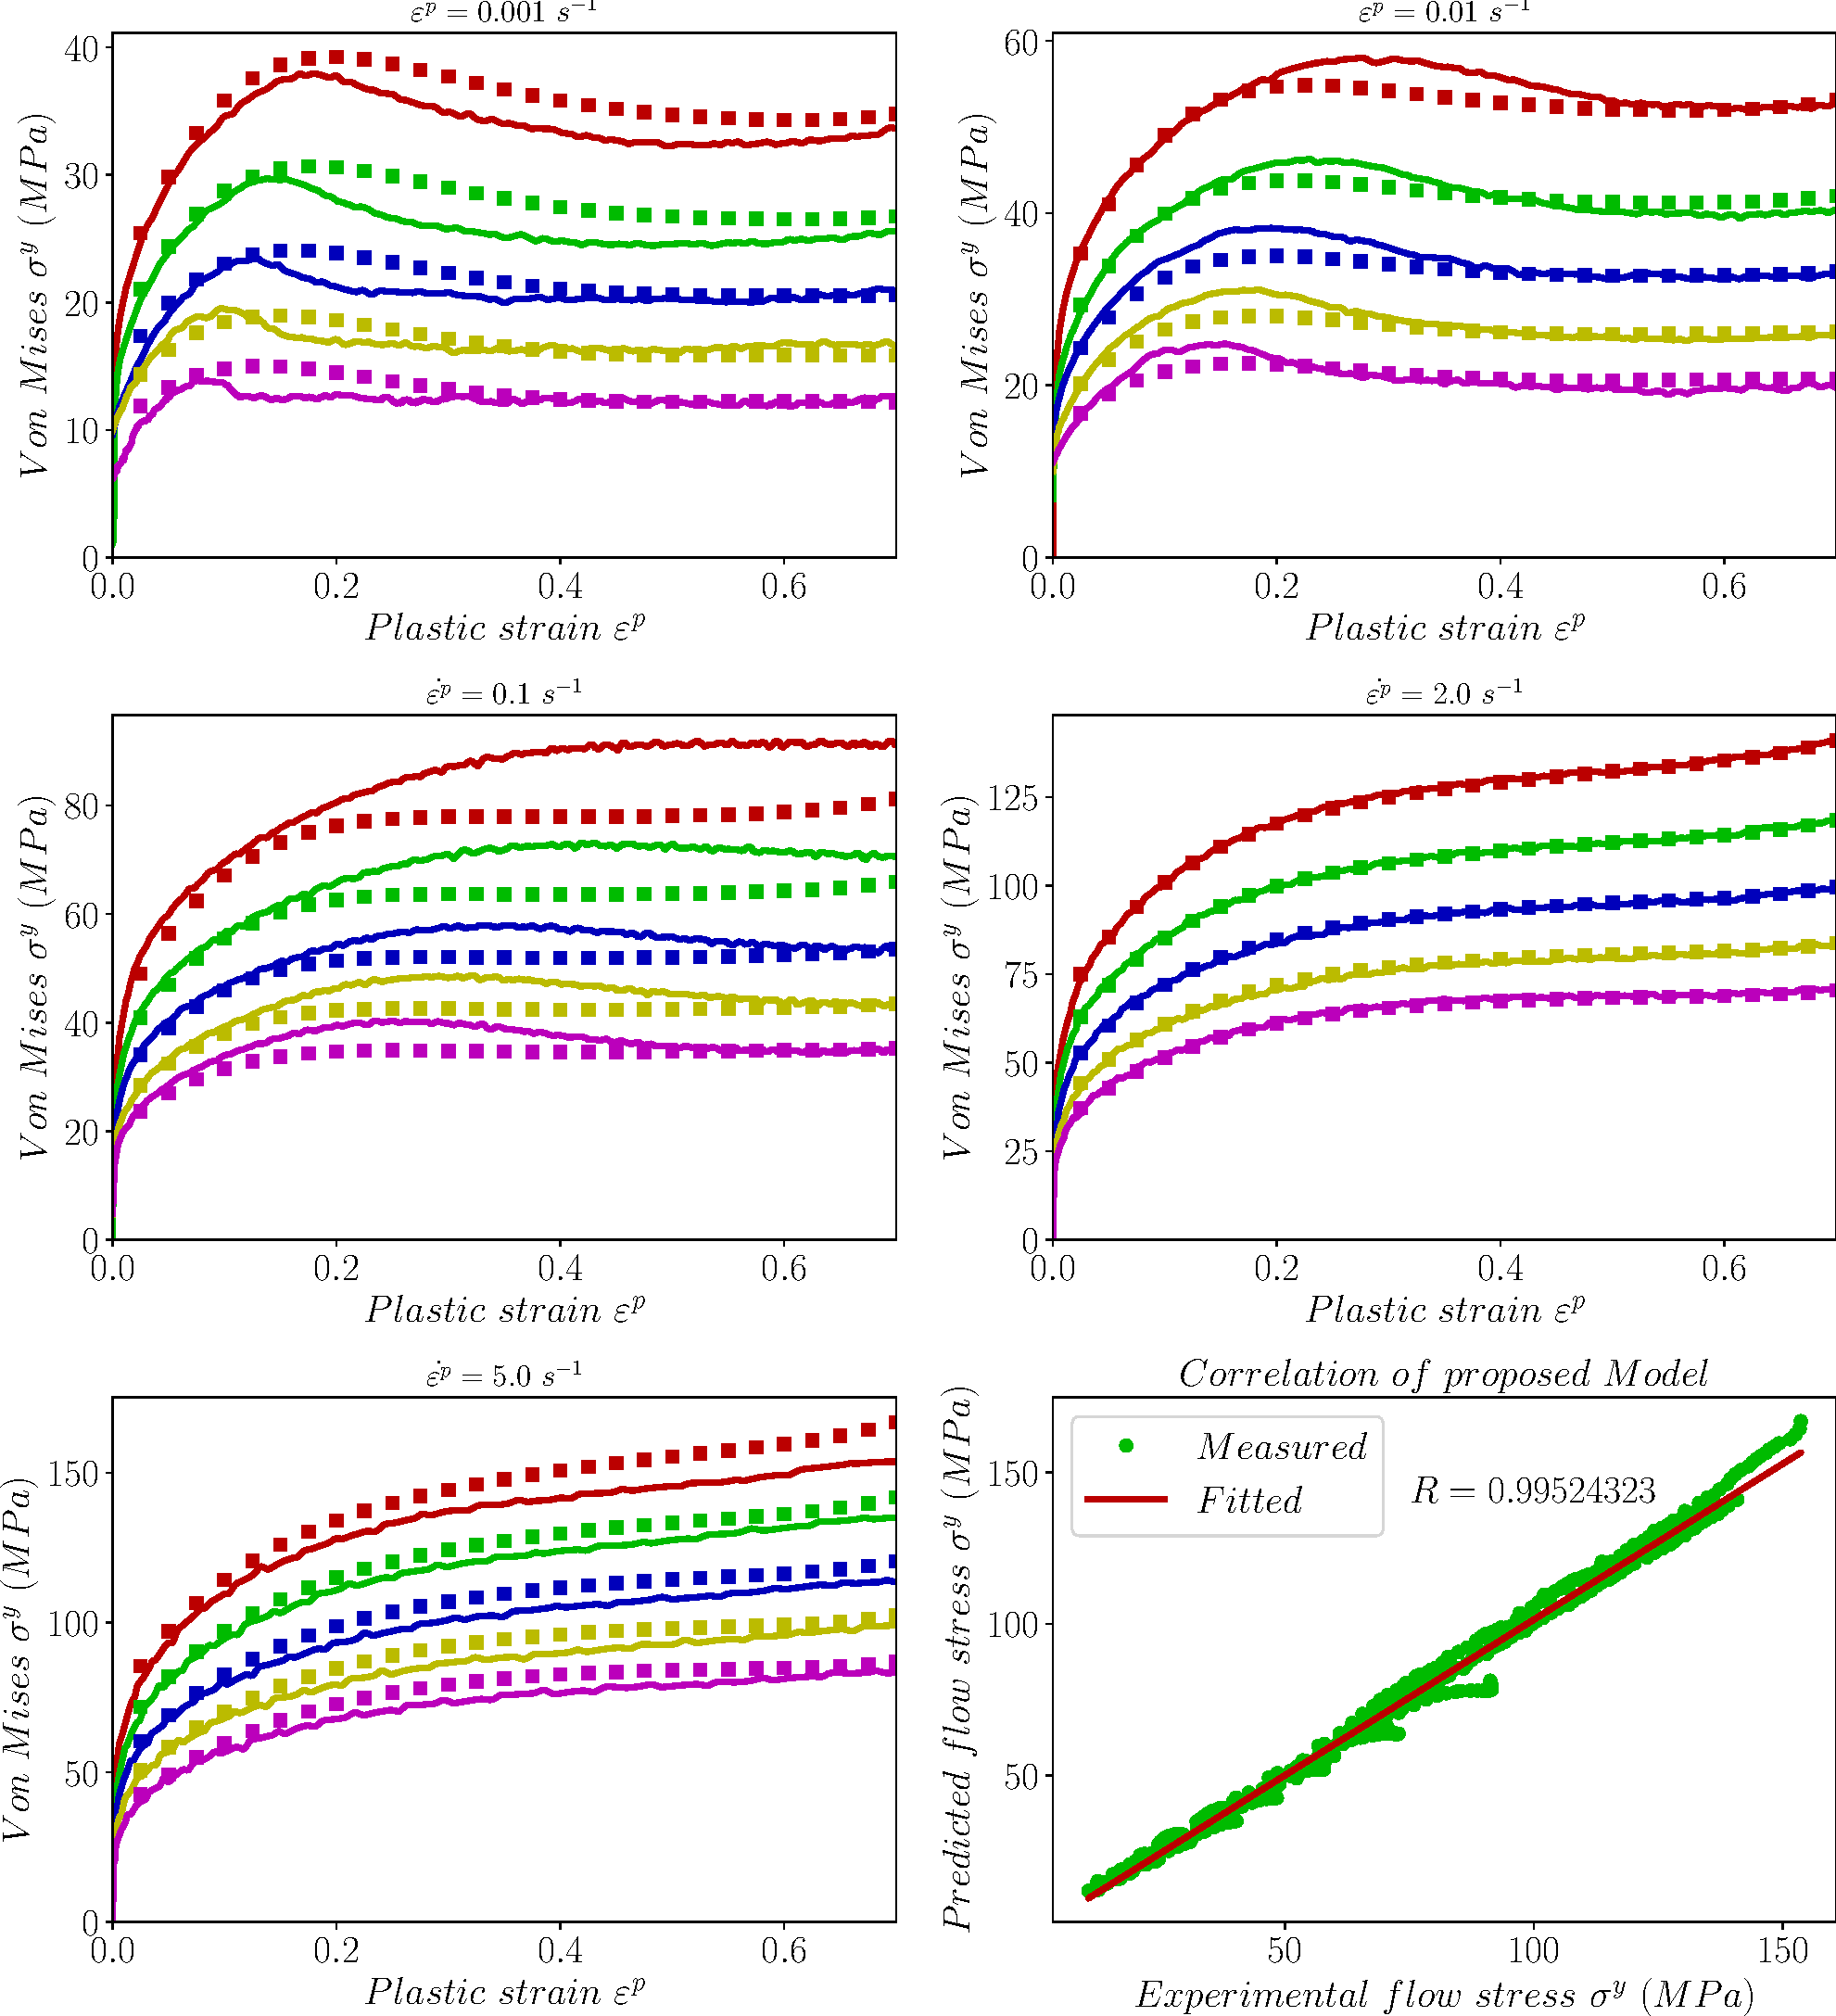
\includegraphics[width=1.02\columnwidth]
{newFigures/iCorrelationPTM}
\caption{Comparison between the experimental and predicted flow stresses by PTM model for interpolation estimation}
\label{fig:iCorrelationPTM}
\end{figure}
\begin{figure}[!ht]
\centering
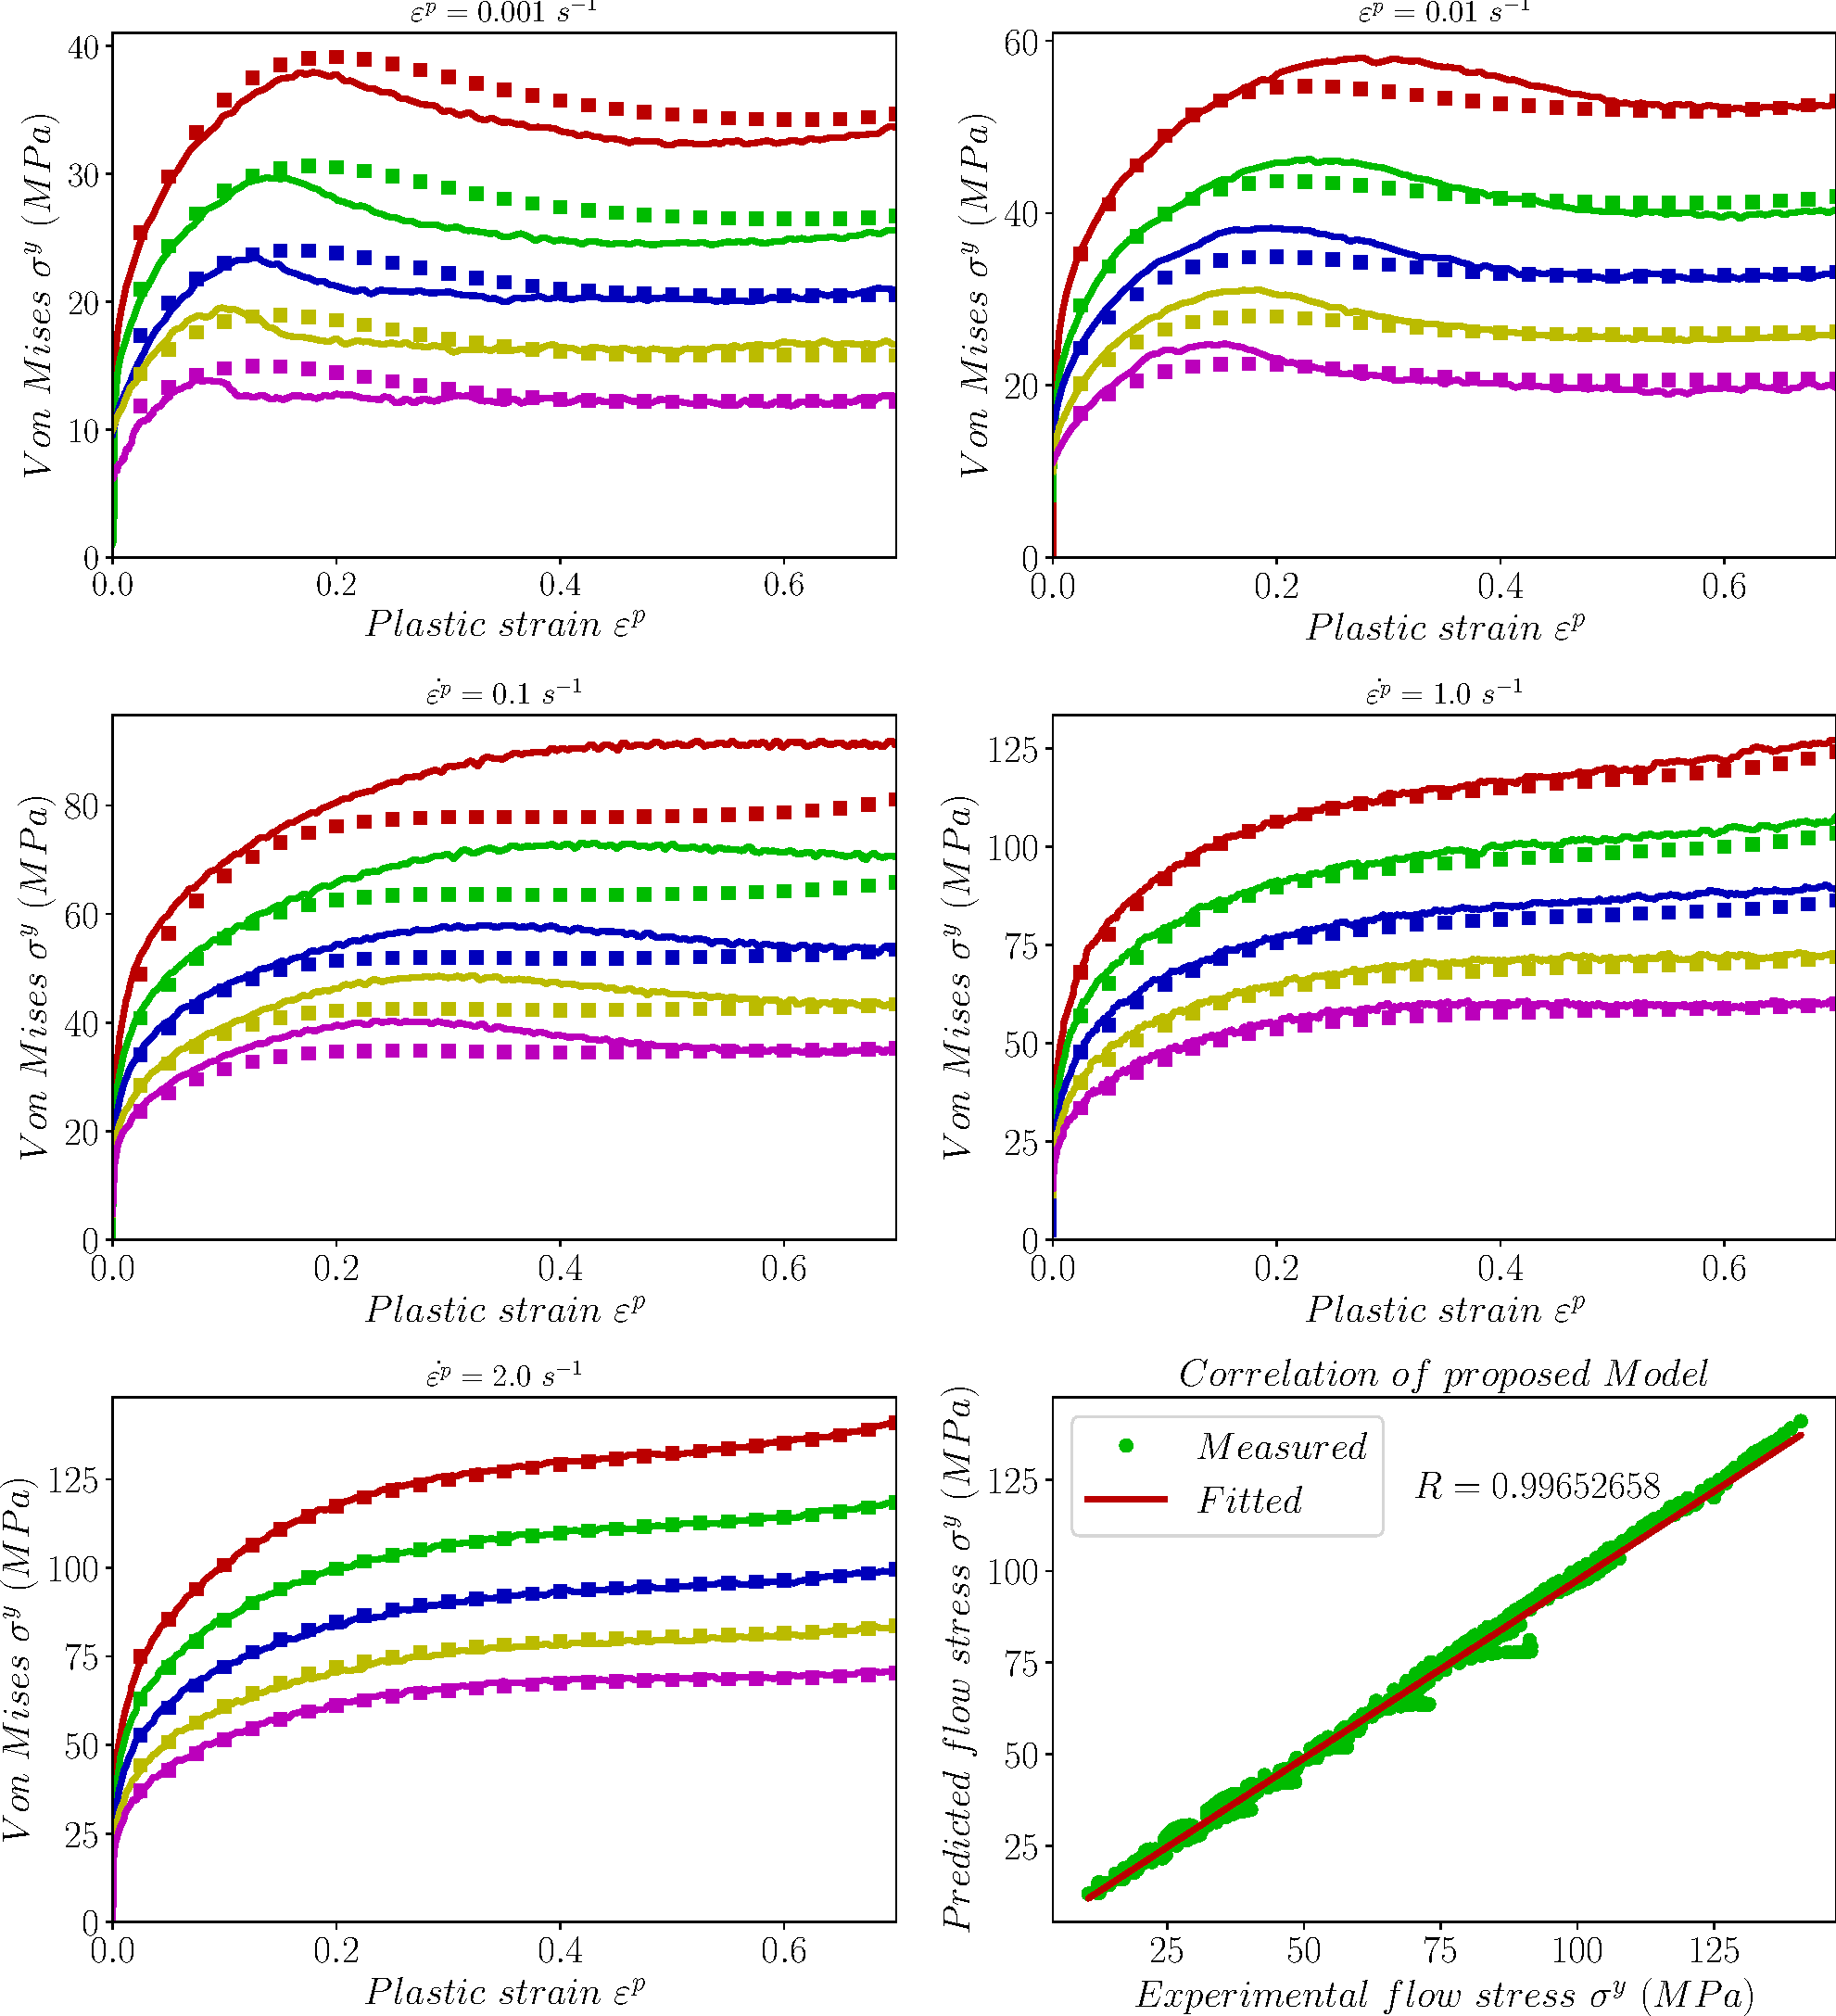
\includegraphics[width=1.02\columnwidth]
{newFigures/eCorrelationPTM}
\caption{Comparison between the experimental and predicted flow stresses by PTM model for extrapolation estimation}
\label{fig:eCorrelationPTM}
\end{figure}

\begin{table}[!h]
\centering{}
\caption{Parameters of the proposed model\label{tab:PTM-parameters}}
\scalebox{1.2}{
\begin{tabular}{ccc}
\hline
&  & \\
Parameters & Interpolation &Extrapolation\\
&  & \\
\hline
$A_0 (\text{MPa})$ & $62.314$ & $62.314$\\
$A_1 (\text{MPa})$ & $559.827$ & $559.827$\\
$A_2 (\text{MPa})$ & $-2160.03$ & $-2160.03$\\
$A_3 (\text{MPa})$ & $4641.94,$ & $4641.94$\\
$A_4 (\text{MPa})$ & $-5193.06$ & $-5193.06$\\
$A_5 (\text{MPa})$ & $2379.1$ & $2379.1$\\
$B_0 $ & $-0.0035805$ & $-0.0035805$\\
$B_1 $ & $0.00282334$ & $0.00282334$\\
$B_2 $ & $-0.00775301$ & $-0.00775301$\\
$B_3 $ & $0.0085135$ & $0.0085135$\\
$B_4 $ & $-0.00412815$ & $-0.00412815$\\
$C_0^0 $ & $0.148539$ & $0.148766$\\
$C_0^1 $ & $-0.302363$ & $-0.304798$\\
$C_0^2 $ & $2.25845$ & $2.2891$\\
$C_0^3 $ & $-5.2651$ & $-5.36673$\\
$C_0^4 $ & $5.38382$ & $5.51053$\\
$C_0^5 $ & $-2.05958$ & $-2.1115$\\
$C_1^0 $ & $-4.3271\ \times10^{-7}$& $-9.92159\ \times10^{-7}$\\
$C_1^1 $ & $0.00165983$& $0.00166581$\\
$C_1^2 $ & $-0.00269801$ & $-0.00272071$\\
$C_1^3 $ & $-0.000132085$& $-8.59293\ \times10^{-5}$\\
$C_1^4 $ & $0.00182935$ & $0.00178989$\\
\hline
\end{tabular}}
\end{table}
%-------------------------------------------------------------------------
\subsection{Artificial neural network model\label{sec:ANNmodel}}
%--------------------------------------------------------------------------
The Artificial Neural Network model (ANN) is a mathematical formulation widely used in many fields today for better prediction. It is a model based on the principle of minimisation where it improves from the progressive decrease of the error during the learning process. Typically an ANN model contains an input layer, an output layer and hidden layers. Each hidden layer is connected to the one before it and the one after it via neurons. Indeed, all neurons in the $k$ layer are connected to each neuron in the ($k+1$ ) layer. To each layer is added another parameter called bias. As said the principle of the ANN model is therefore based on the minimisation of the difference between the value obtained from the output of the network and the expected value.  Indeed, once the error is calculated, it is propagated back to the input layer in order to update the model parameters via the minimisation algorithms. In our case, the ADAM algorithm is used. The architecture of the network used in this study is shown in Figure \ref{fig:ANN-scheme-2HL}. After several tests of different types of network architecture, it was found that two hidden layers including $15$ neurons for the first hidden layer and $7$ for the second one gives the best prediction as well as for interpolation and extrapolation where the input layer is composed of three neurons ($\varepsilon^p$, $\mdot{\varepsilon}^p$, $T$) and the output layer is composed of a single neuron corresponding to the flow stress. The good performance of the model is found to be stable between $800$ and $1000$ epochs. This number was therefore used to train the model for both interpolation prediction and extrapolation. 

In this study $700$ of data were used; $80\%$ (560) are randomly selected for training and $20\%$ (140) for testing. Before learning, a normalisation of the data is required in order to have all data between $0$ and $1$. The Equation is widely used for normalization.
\begin{equation}
X_n = \frac{X - X_{min}}{X_{max} - X_{min}}
\end{equation}
Where $X$ is the orginal data ($\varepsilon^p$, $\log(\mdot{\varepsilon}^p/\varepsilon_0$,  $T$, $\sigma^y$), $X_{min}$ and $X_{max}$ are the minimum and maximum values of $X$ respectively. $X_n$ is the normalized data of the corresponding $X$. The trained model once tested can be used to predict the behaviour of the AISI P20 alloy. Figure and Figure show a comparison between the predicted flow stresses from ANN model and measured data from hot compression test as well as for interpolation prediction and extrapolation prediction. As shown from these two figures, the correlation between the experimental and the ANN prediction based is very good over the full range of data and the predicted data can well track the hardening and softening regions of the hot deforming material. Therefore, the ANN model can be used to simulate the hot deformation of this type of alloy. This was not necessarily the case with the analytical models. The performance of this prediction will be much more appreciated when it comes to testing its ability to predict data that has not been used in either the training or the test data, but rather a full-fledged trial that we wish to validate the ANN prediction by experimental. This validation will be done both with a strain rate between those used in the training and in this case we will validate the interpolation and outside of the strain rates used in the training and in this case we will validate the extrapolation.
\begin{figure}[!ht]
\centering
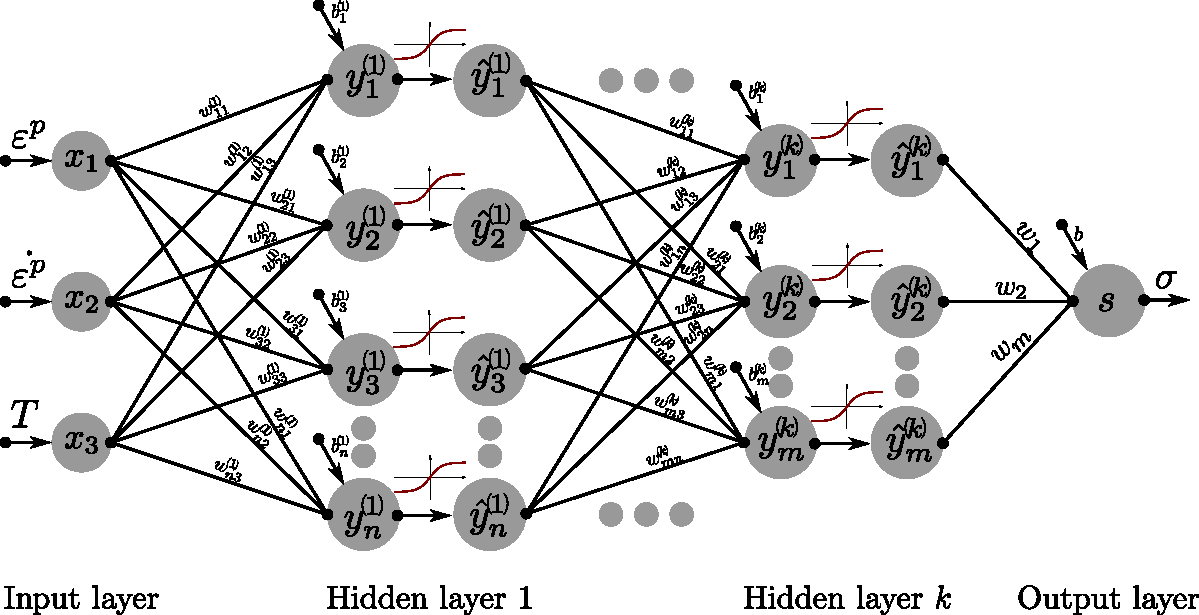
\includegraphics[width=0.9\columnwidth]
{newFigures/ANN-scheme-2HL}
\caption{Multi-layer Artificial Neural Network architecture \cite{OPantale-2021-LGP}.}
\label{fig:ANN-scheme-2HL}
\end{figure}
\begin{figure}[!ht]
\centering
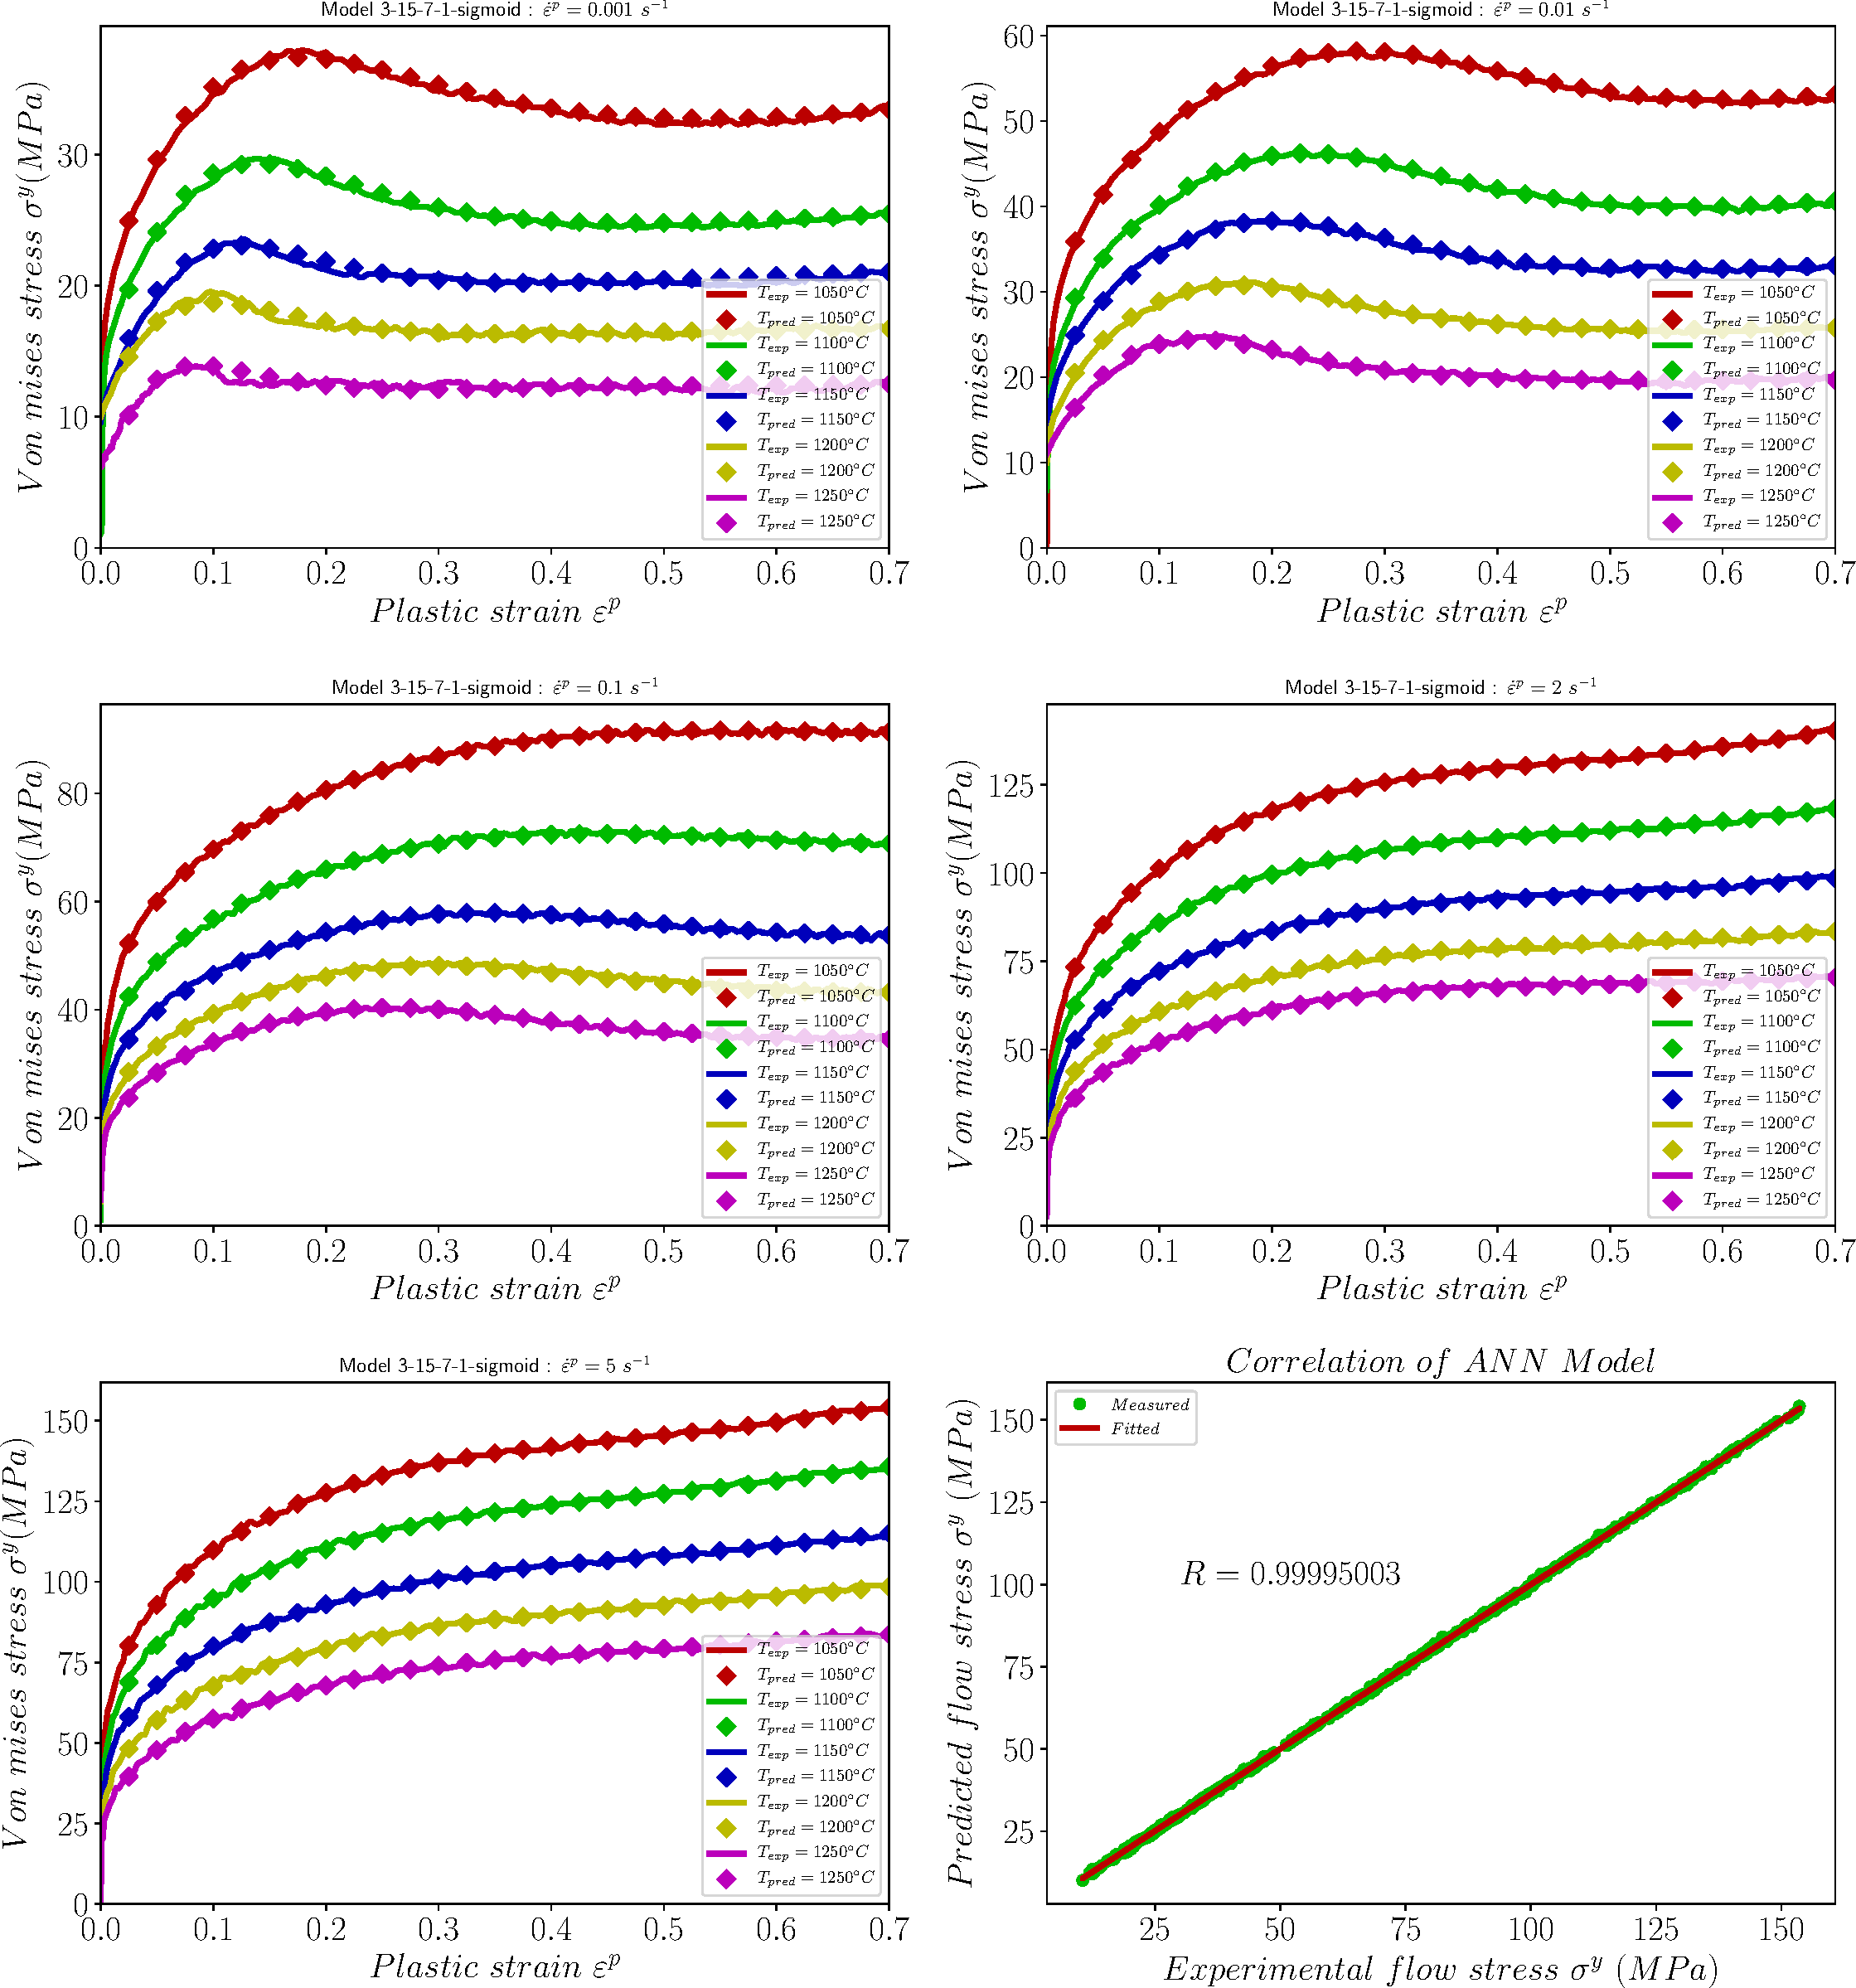
\includegraphics[width=1.02\columnwidth]
{newFigures/iCorrelationANN}
\caption{Comparison between the experimental and predicted flow stresses by ANN model for interpolation estimation}
\label{fig:iCorrelationANN}
\end{figure}
\begin{figure}[!ht]
\centering
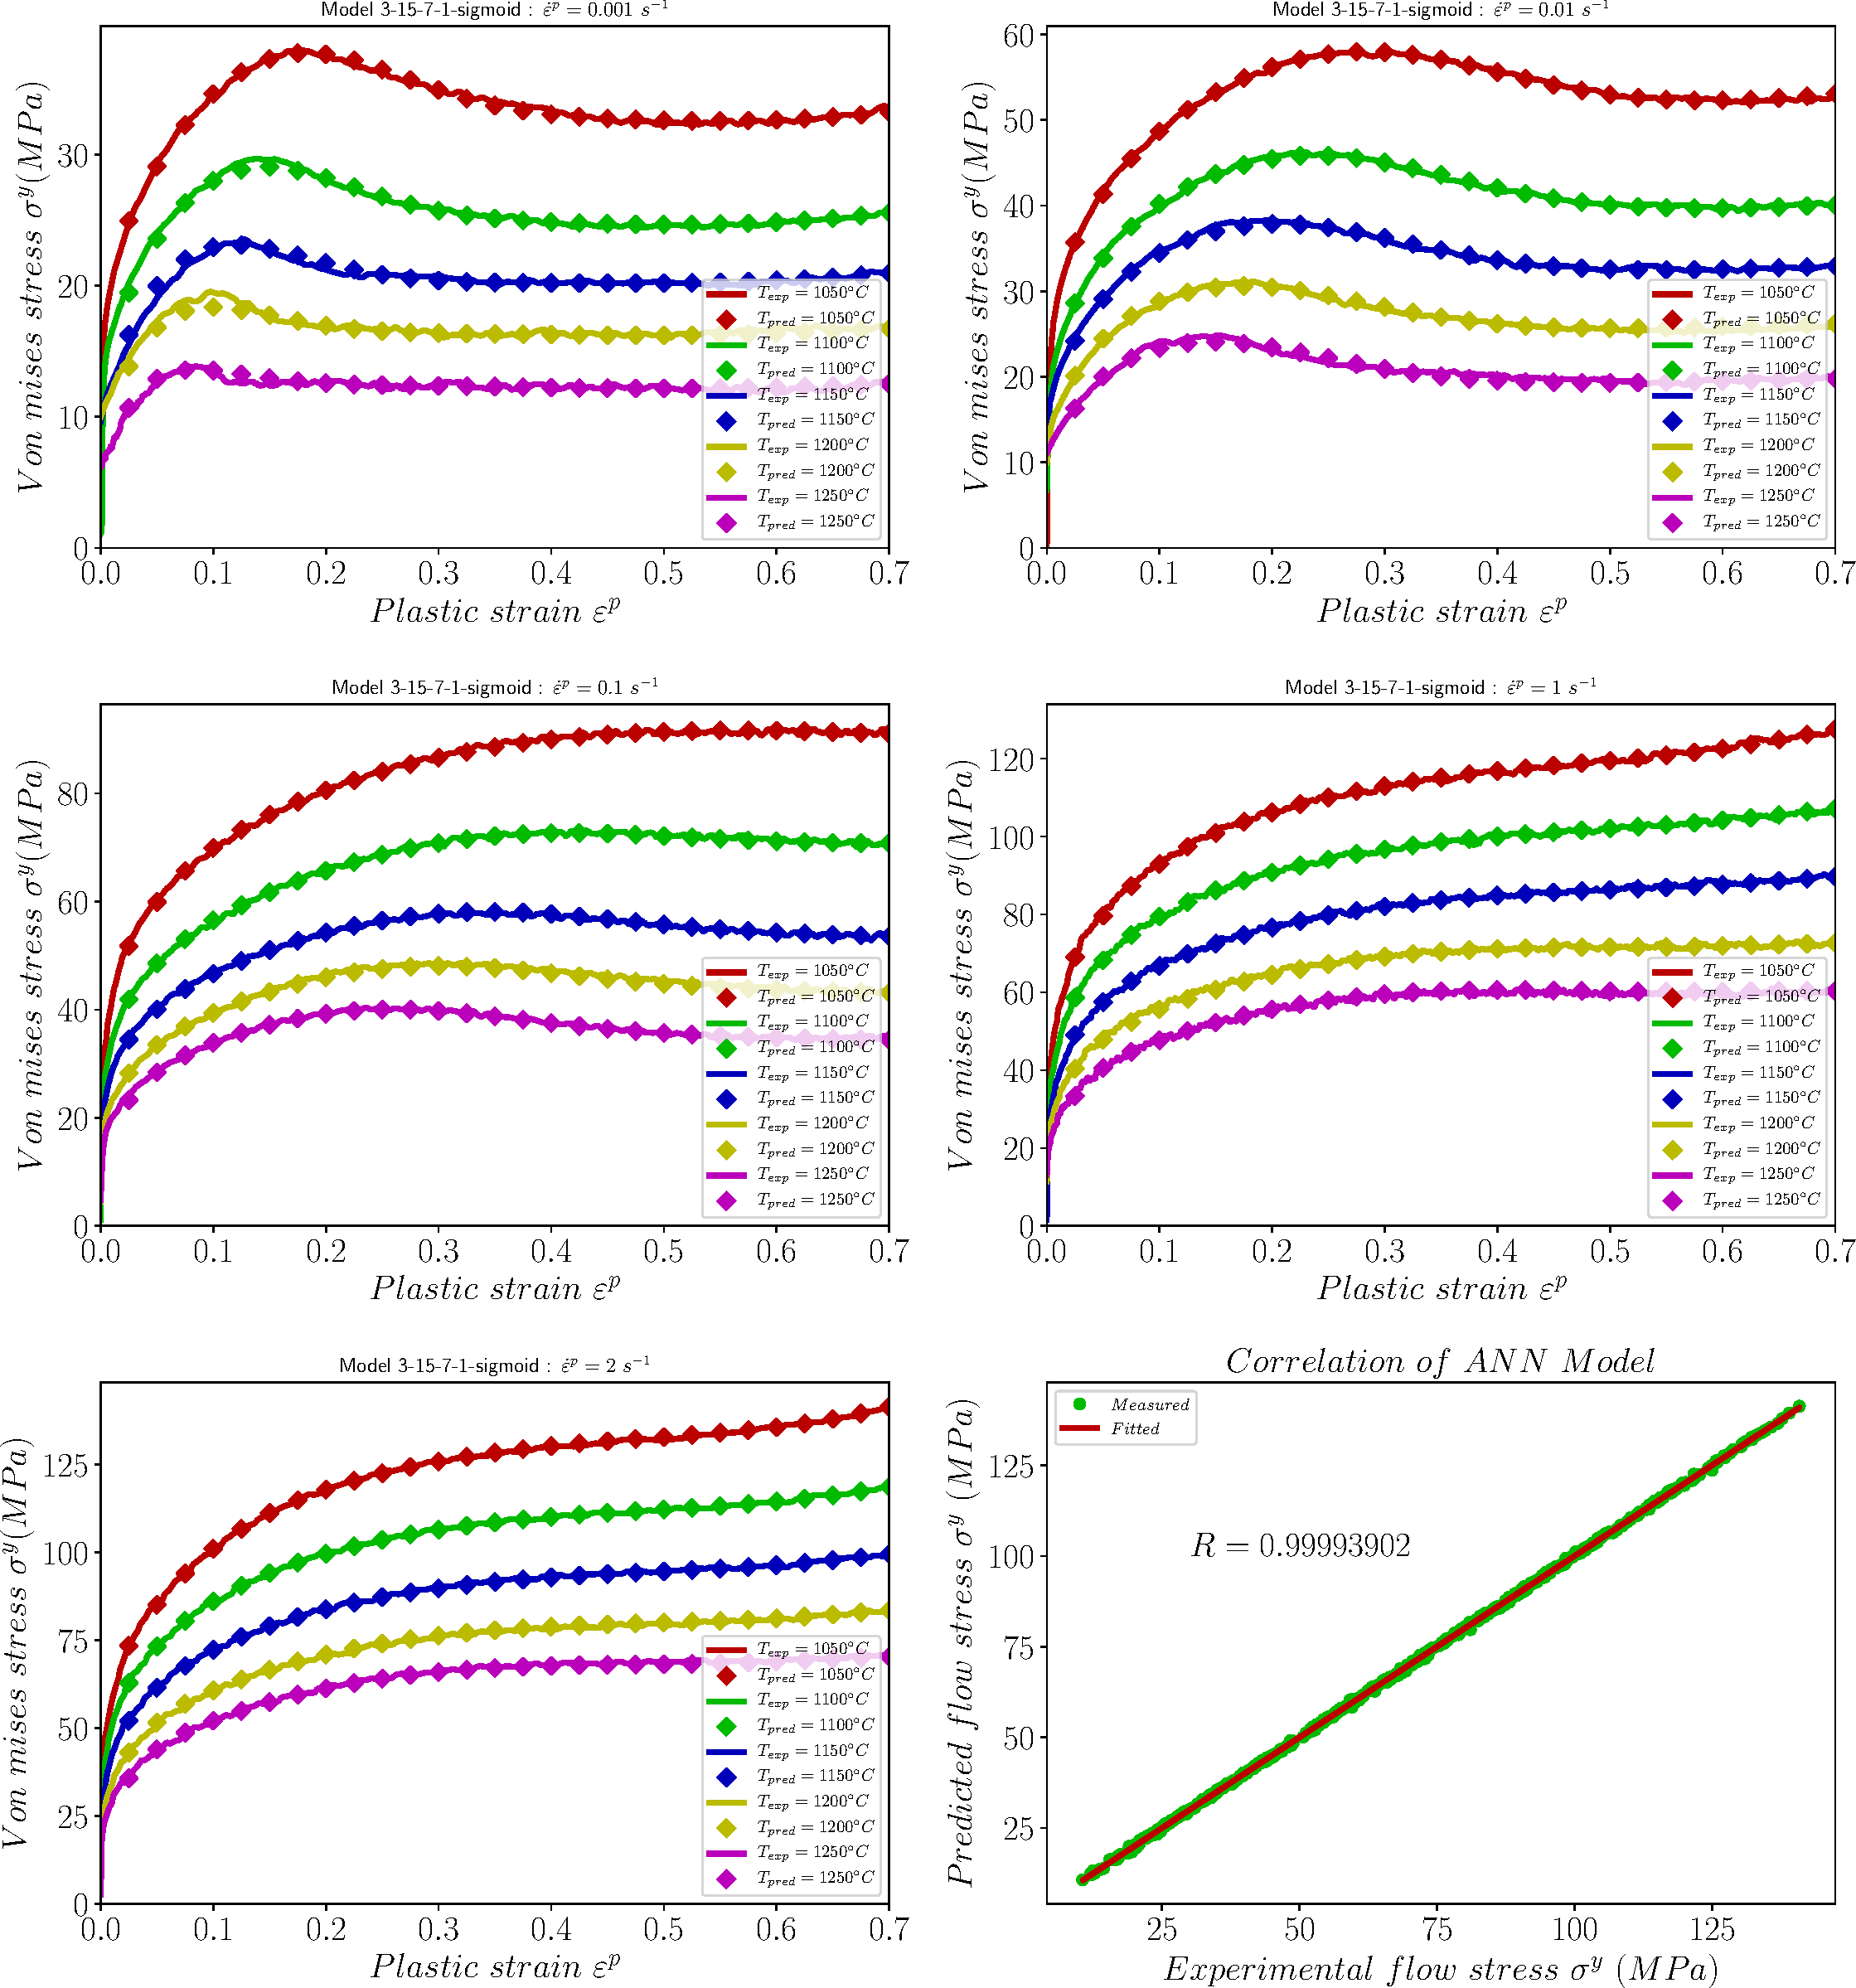
\includegraphics[width=1.02\columnwidth]
{newFigures/eCorrelationANN}
\caption{Comparison between the experimental and predicted flow stresses by ANN model for extrapolation estimation}
\label{fig:eCorrelationANN}
\end{figure}

%-------------------------------------------------------------------------
\subsection{Comparison of analytical and ANN models\label{sec:Comparison}}
%--------------------------------------------------------------------------
%-------------------------------------------------------------------------
\subsubsection{Identification results' comparison \label{sec:Interpolation}}
%--------------------------------------------------------------------------
The accuracy and predictive ability of both analytical and ANN models are generally assessed by some coefficients such as the correlation coefficient ($R$) (Equation (\ref{eq:R-expression})), Average Absolute Relative Error ($AARE$ generally known as $\AARE$ ) (Equation (\ref{eq:AARE-expression})) and Root Mean Square Error ($RMSE$) (Equation (\ref{eq:RMSE-expression})).
\begin{equation}
\label{eq:R-expression}
\R(\%) = \frac{\displaystyle\sum_{i=1}^{N}{\left(E_i - \overline{E}\right)\left(P_i - \overline{P}\right)}}{\sqrt{\displaystyle\sum_{i=1}^{N}\left(E_i - \overline{E}\right)^2 .\displaystyle\sum_{i=1}^{N}\left(P_i - \overline{P}\right)^2}}\times 100
\end{equation}
\begin{equation}
\label{eq:AARE-expression}
\AARE(\%) = \frac{1}{N}\displaystyle\sum_{i=1}^{N} \displaystyle\left\lvert\frac{E_i- P_i}{E_i} \right\rvert\times 100
\end{equation}
\begin{equation}
\label{eq:RMSE-expression}
RMSE (\%) = \sqrt{\frac{1}{N} \displaystyle\sum_{i=1}^{N} \left(E_i - P_i\right)^2} \times 100
\end{equation}
Where $E_i$ is the experimental value and $P_i$ is the predicted value of the constitutive law (phenomenological and ANN models), $\overline{E}$ and $\overline{P}$ are the mean values of the experimental and predicted values, respectively.

The correlation coefficient $R$ is generally used to show the degree of linearity between the experimental and predicted values. The model sometimes tends to be biased towards low and high values. Therefore, a good (high) value of $R$ does not necessarily mean a good prediction of the model but simply establishes a good linearity correlation between the experiment and the prediction \cite{phaniraj2003applicability}. On the other hand, other coefficients ($\AARE$ and $RMSE$) are used to estimate the predictive capacity of the model because they are considered unbiased as well as for low and high values. Indeed, they verify the predictability of a model term by term comparison of the relative error in relation to the real value of the variable \cite{srinivasulu2006comparative}. In the previous sections the correlations between the experimental flow stresses and those provided by the phenomenological and ANN models have been presented and the correlation coefficients $R$ for JC, MZA, HS, Arhenius, proposed and ANN models are $0.98405682$, $0.98786324$, $0.98413109$, $0.99829876$, $0.99524323$ and $0.99995003$, respectively in case of prediction for interpolation validation. These results show the Arrhenius-type, proposed and ANN models have better correlation between the experimental data and predicted results compared with the JC, MZA and HS models.

All coefficients for evaluating the high-temperature flow stress prediction capability of the AISI P20 alloy for all models presented in this work are summarized in the Table \ref{tab:Coefsparams}. From this Table, it can be seen that the ANN model has a good prediction than the analytical models. All this shows sufficiently that the ANN model is more effective in describing the behaviour of the AISI P20 alloy for high temperature deformation. This efficiency will therefore be validated on tests at two different selected strain rates. One between the minimum and the maximum strain rates used during identification or training for ANN model and another one outside higher than the maximum strain rate. This will validate the interpolation and extrapolation capability of the analytical and phenomenological models. The prediction results should lead to a better interpolation and extrapolation capability of the ANN model than phenomenological models as shown during identification step. The following sections will focus on this analysis.

Another thing to be analysed from this table is the link between the values of the correlation coefficient $R$ and the values of $\AARE$. Indeed, as mentioned above, the $R$ coefficient does not necessarily mean a good prediction of the model but a good relationship of linearity between the experiment and the prediction. To ensure a good prediction of the model, it is necessary to add to $R$, the values of $\AARE$. For example and in the case of identification for the validation of the interpolation (the same analysis can be done for the validation of the extrapolation), let us observe carefully taht, the values of the coefficients $R$ are $99.0145\%$, $98.4131\%$ and those of $\AARE$ are $12.7939\%$ and $8.7309\%$ respectively for the MZA model and the HS model. This seems contradictory when the $R$ of HS is smaller than that of MZA, whereas for the $\AARE$ values it is the opposite case. This simply means that the HS model has a good prediction compared to the MZA model whereas in the framework of the linear correlation between the experiment and the prediction the MZA model makes it better. All this can be seen from the figures where we can observe the HS curves are indeed closer to the experimental than those of MZA while the points are scattered for HS model on the correlation curve. This validates the analysis made by \cite{phaniraj2003applicability, srinivasulu2006comparative} their works. The same analysis can be applied to the other results of the other models, although the ANN model is still the best for a good prediction.
\begin{table}[h!]
\centering{}
\caption{Comparison of phenomenological an ANN models' accurary coefficients}
\scalebox{0.88}{
\begin{tabular}{lccccccc}
\hline
&		&		&         &             &		   &		  &						\\
Coefficients&JC  & MZA  &HS  & Arhenius      & Proposed  &ANN &Expected predictions \\
&				&				&         &             &		   &	     &	    \\
\hline
$R(\%)$&$98.4057$&$99.0145$&$98.4131$&$99.8299$& $99.5243$&$99.9950$&Interpolation  \\
$R(\%)$&$98.2519$&$98.7863$&$98.6493$&$99.7752$& $99.6527$&$99.9939$&Extrapolation  \\
%\hdashline
$\AARE(\%)$&$12.6421$&$12.7939$&$8.7309$&$3.7026$&$4.4781$&$0.6613$&Interpolation   \\
$\AARE(\%)$&$12.7567$&$11.7289$&$7.6883$&$3.7875$&$3.9697$&$0.6219$&Extrapolation   \\
\hline
\label{tab:Coefsparams}
\end{tabular}}
\end{table}
%-------------------------------------------------------------------------
\subsubsection{Interpolation and extrapolation validation\label{sec:Extrapolation}}
%--------------------------------------------------------------------------
This section is devoted to the validation of the models developed in this study. To do so, let us briefly recall the purpose of this work in order to make it much clearly. Indeed, we have developed analytical models and a model based on the neural network for certain values of strain, strain rates and temperatures. The idea is therefore to randomly fix two strain rates while keeping the same values of strains and temperatures used for the development of the phenomenological and ANN models. Of these two strain rates, one must be between the minimum and maximum strain rate values already known and another must be higher. This is to test the interpolation and extrapolation capability of these models in order to validate them by experimental data.
 
For the validation of the interpolation, the chosen strain rate is $\mdot{\varepsilon}^p = 1.0\ \text{s}^{-1}$ and those used for identification (training for ANN) are $\mdot{\varepsilon}^p = 0.001\ \text{s}^{-1}$ , $\mdot{\varepsilon}^p = 0.01\ \text{s}^{-1}$ , $\mdot{\varepsilon}^p = 0.1\ \text{s}^{-1}$, $\mdot{\varepsilon}^p = 2.0\ \text{s}^{-1}$  and $\mdot{\varepsilon}^p = 5.0\ \text{s}^{-1}$. The Figure \ref{fig:inCombinaison1} and Figure \ref{fig:inCombinaison2} show the comparison between the predictions of the analytical and ANN models and the experiment. It appears from these Figures that all models have relatively good predictions but the ANN model remains the best because the value of its $\AARE$ is $1.4\%$ while it is between $2.33\%$ and $6.13\%$ for the analytical models. This further shows the performance of the ANN model compared to the analytical models. All these results are summarised in Table \ref{tab:CoefInEx}.
\begin{figure}[!ht]
\centering
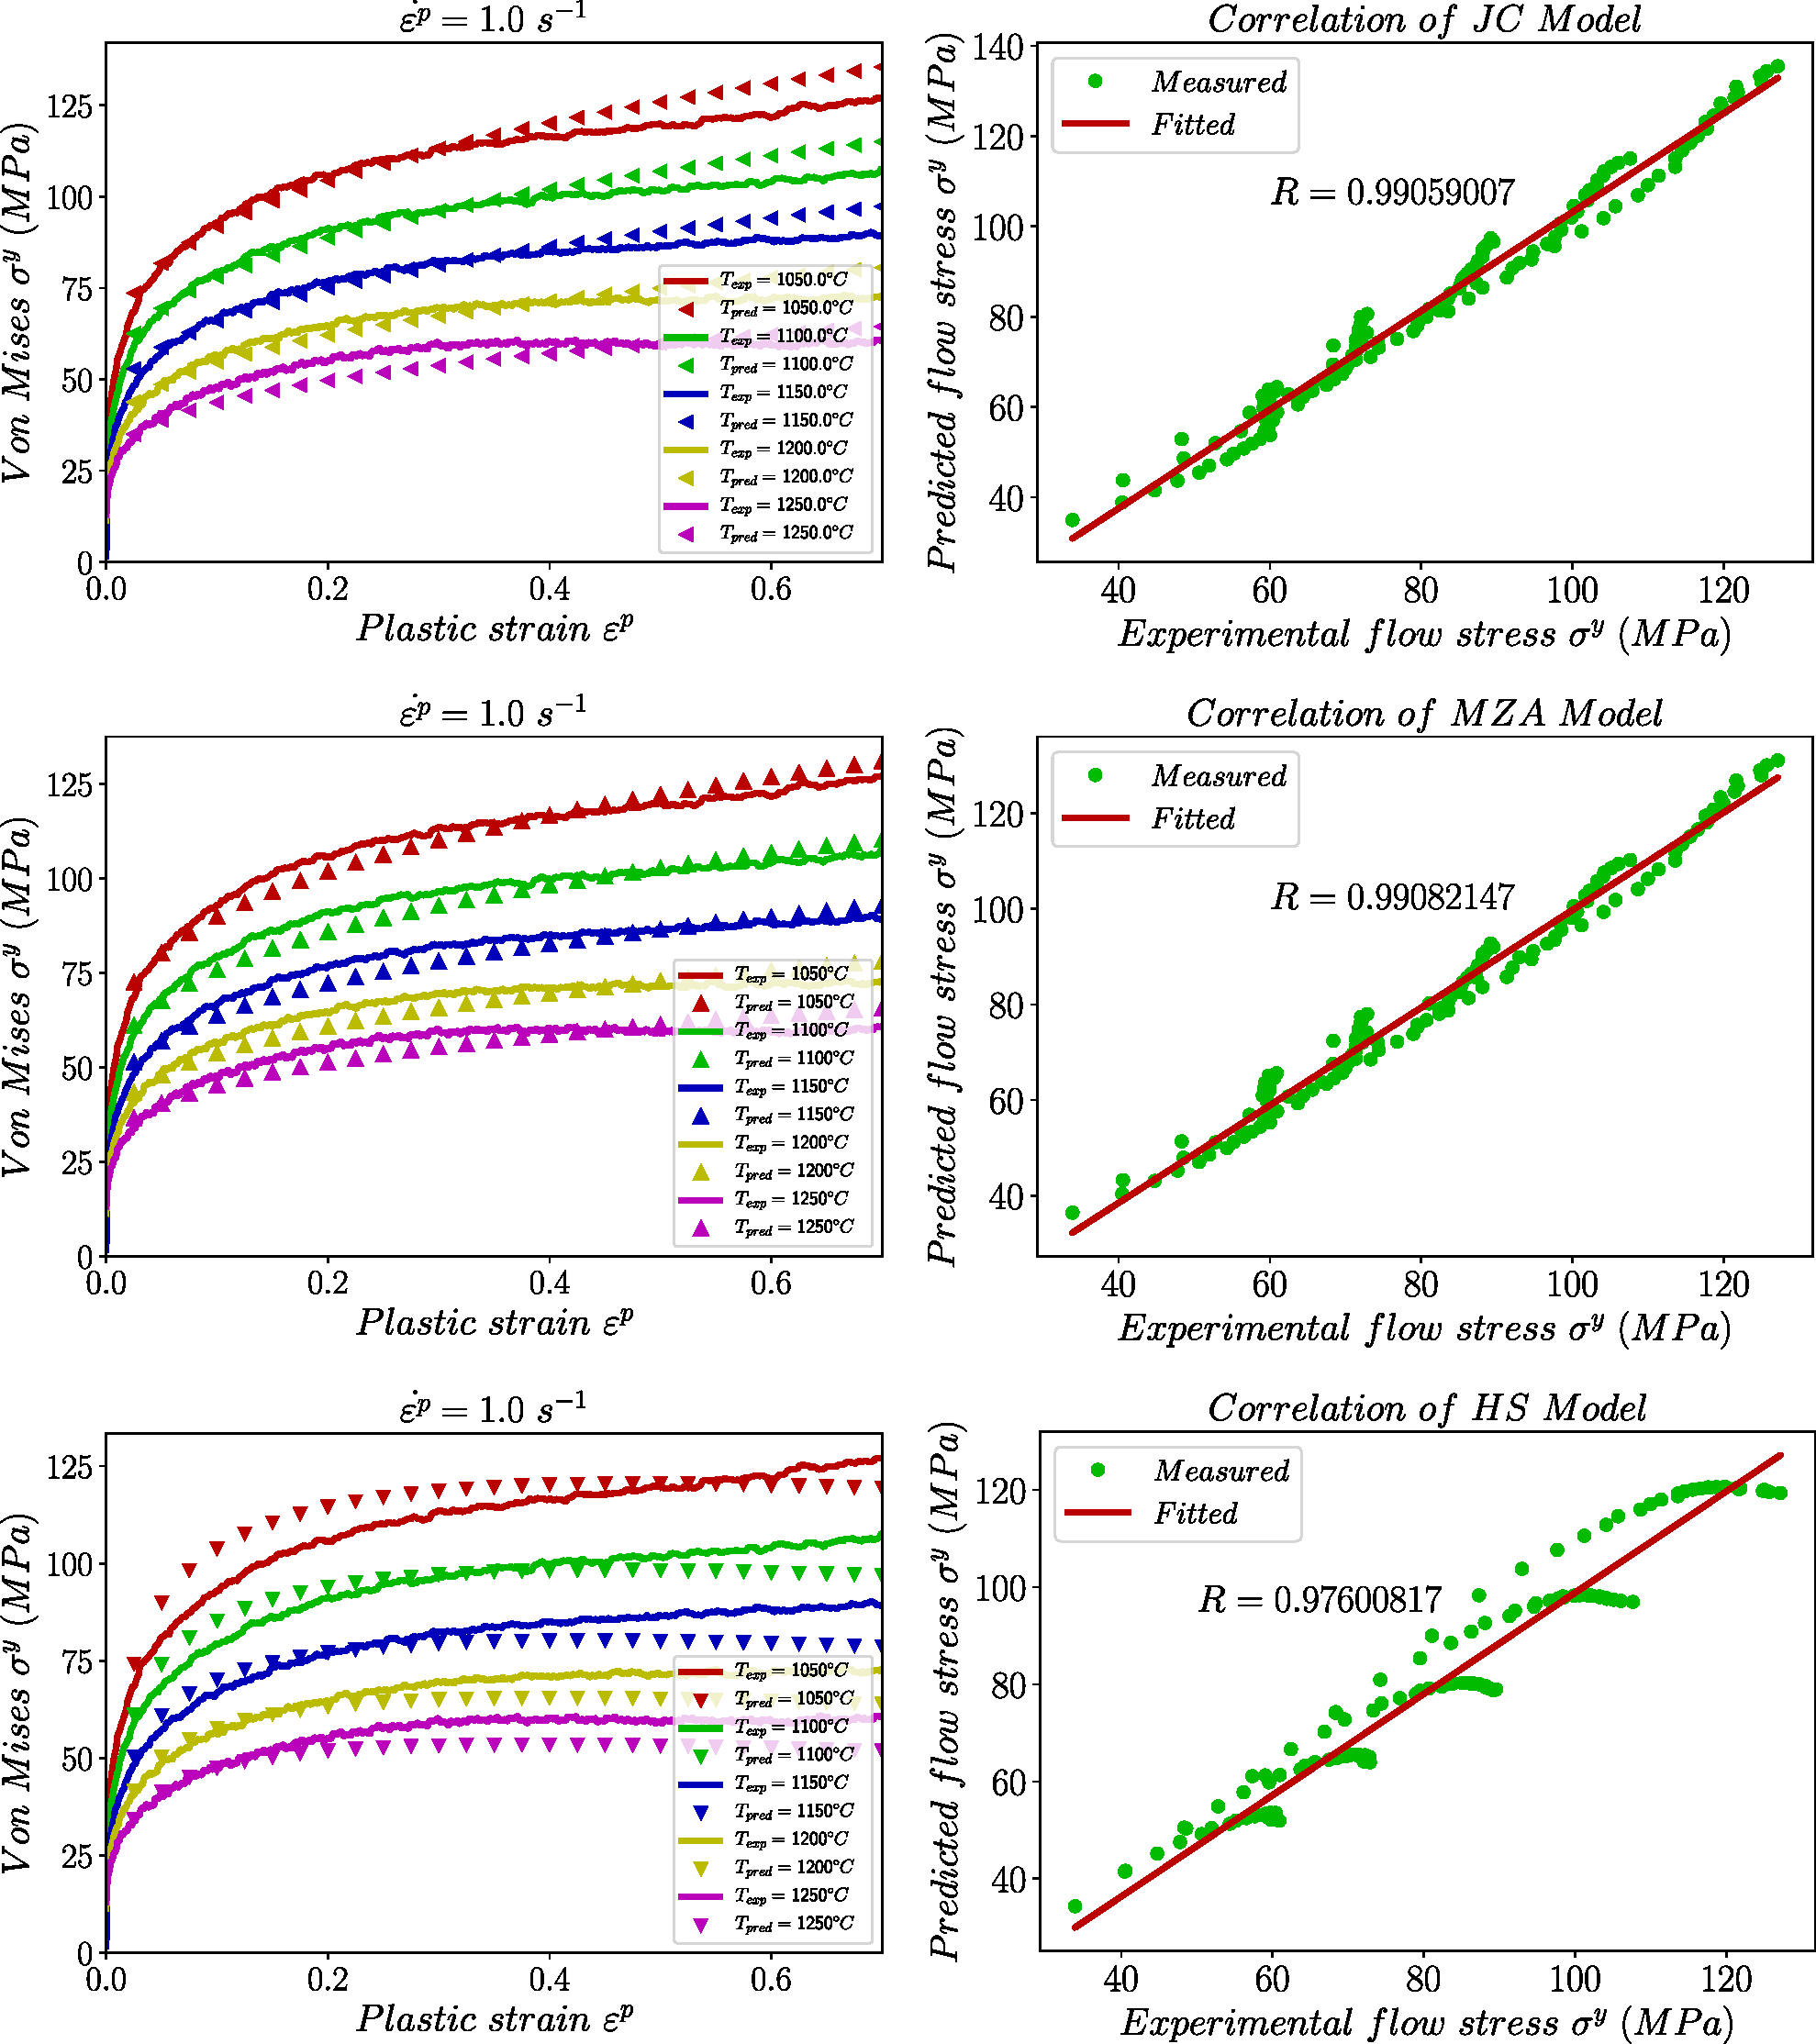
\includegraphics[width=1.02\columnwidth]
{newFigures/inCombinaison1}
\caption{Comparison between the experimental and predicted flow stresses by ANN model for extrapolation estimation}
\label{fig:inCombinaison1}
\end{figure}
For the validation of the extrapolation, the chosen strain rate is $\mdot{\varepsilon}^p = 5.0\ \text{s}^{-1}$ and those used for identification (training for ANN) are $\mdot{\varepsilon}^p = 0.001\ \text{s}^{-1}$ , $\mdot{\varepsilon}^p = 0.01\ \text{s}^{-1}$ , $\mdot{\varepsilon}^p = 0.1\ \text{s}^{-1}$, $\mdot{\varepsilon}^p = 1.0\ \text{s}^{-1}$  and $\mdot{\varepsilon}^p = 2.0\ \text{s}^{-1}$. Figure \ref{fig:exCombinaison1} and Figure \ref{fig:exCombinaison2} show the comparison between the predictions  and the experimental. Unlike interpolation, the predictions of the analytical models are not very good because the errors are between $3.2\%$ and $12.99\%$ while that of the ANN model is $1.74\%$. Again, the ANN model shows its ability to extrapolate data. This makes it possible to say that the ANN model remains the best tool to characterize the behaviour of a material subjected to certain deformation conditions. It can also be noted that the Arhenius and the proposed models still have some ability to extrapolate because their $\AARE$ are respectively $ 3.2 \% $ and $ 3.78 \%$; which is not bad.
\begin{figure}[!ht]
\centering
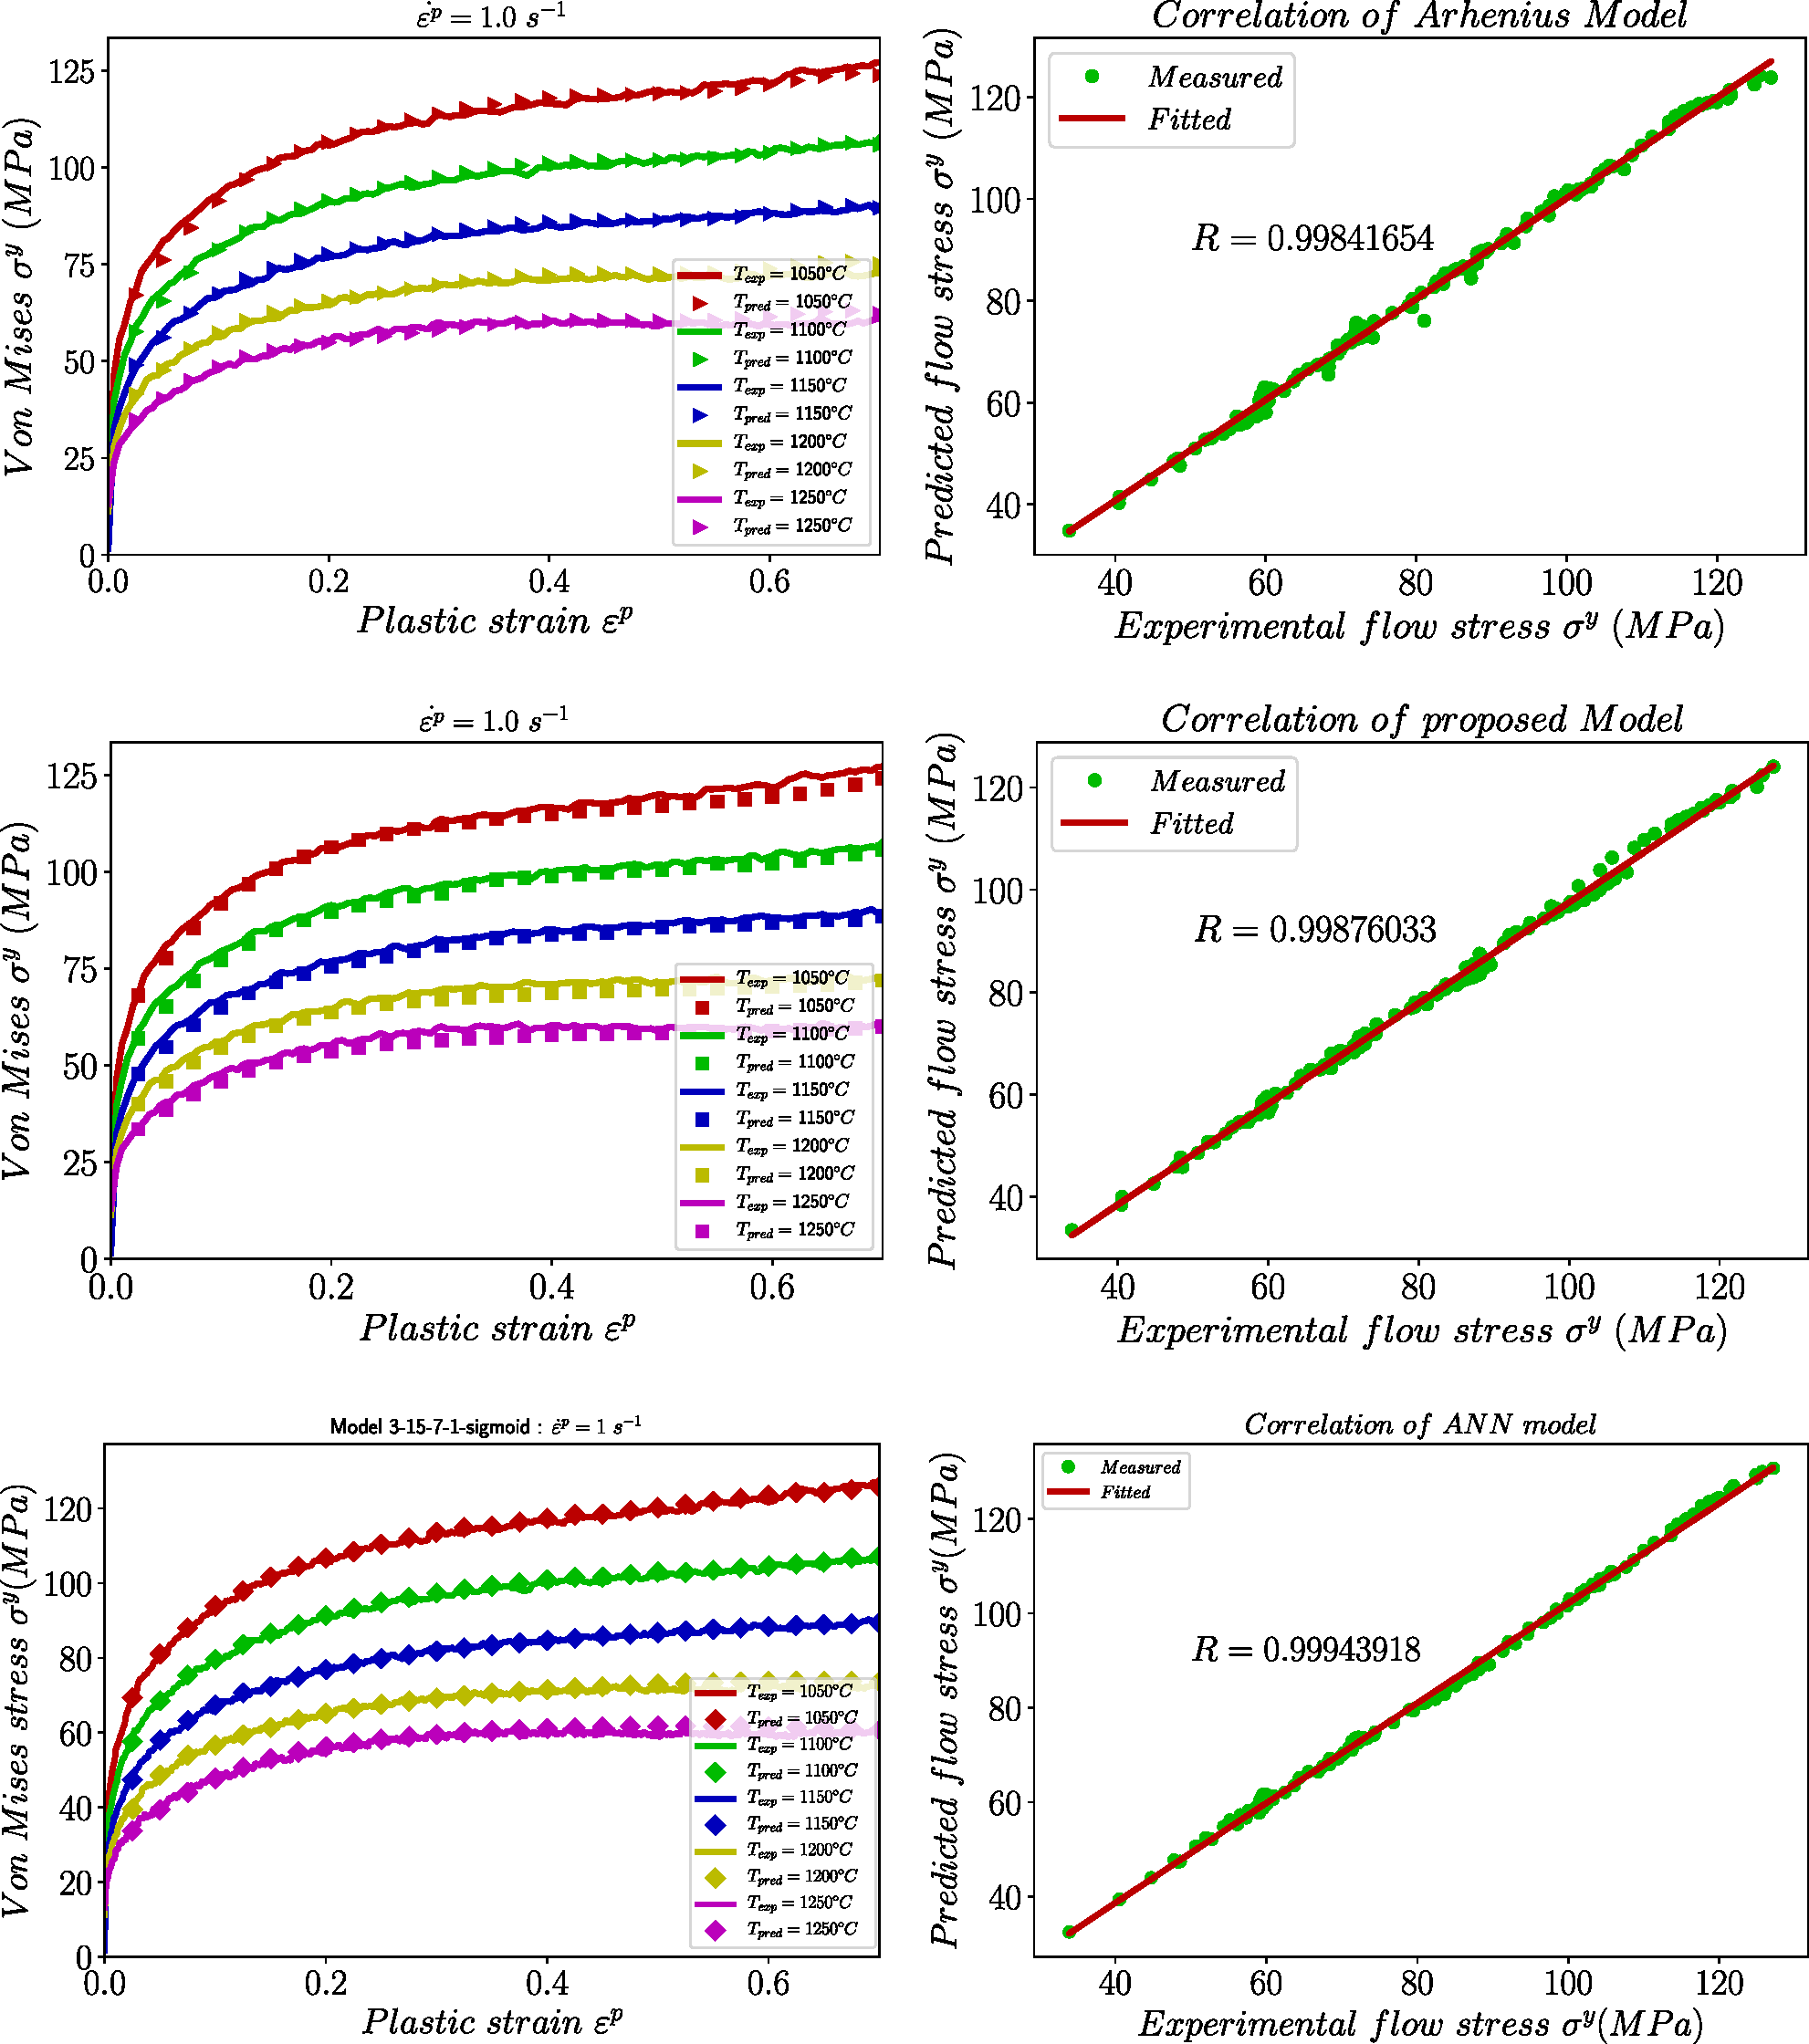
\includegraphics[width=1.02\columnwidth]
{newFigures/inCombinaison2}
\caption{Comparison between the experimental and predicted flow stresses by ANN model for extrapolation estimation}
\label{fig:inCombinaison2}
\end{figure}
\FloatBarrier
\begin{table}[h!]
\centering{}
\caption{Validatio of interpolation and extrapolation accurary coefficients}
\scalebox{0.92}{
\begin{tabular}{lccccccc}
\hline
&		&		&         &             &		   &		  &						\\
Coefficients&JC  & MZA  &HS  & Arhenius      & Proposed  &ANN &Validations 		    \\
&				&				&         &             &		   &	     &	    \\
\hline
$R(\%)$&$99.0590$&$99.0821$&$97.6008$&$99.8417$& $99.8760$&$99.9439$&Interpolation  \\
$R(\%)$&$99.2920$&$99.4879$&$93.9429$&$99.6870$& $99.7582$&$99.8047$&Extrapolation  \\
%\hdashline
$\AARE(\%)$&$4.2686$&$3.7440$&$6.1391$&$2.3321$&$2.7590$&$1.4018$&Interpolation   \\
$\AARE(\%)$&$4.8988$&$3.4506$&$12.9939$&$3.2008$&$3.8845$&$1.7433$&Extrapolation   \\
\hline
\label{tab:CoefInEx}
\end{tabular}}
\end{table}
\begin{figure}[!ht]
\centering
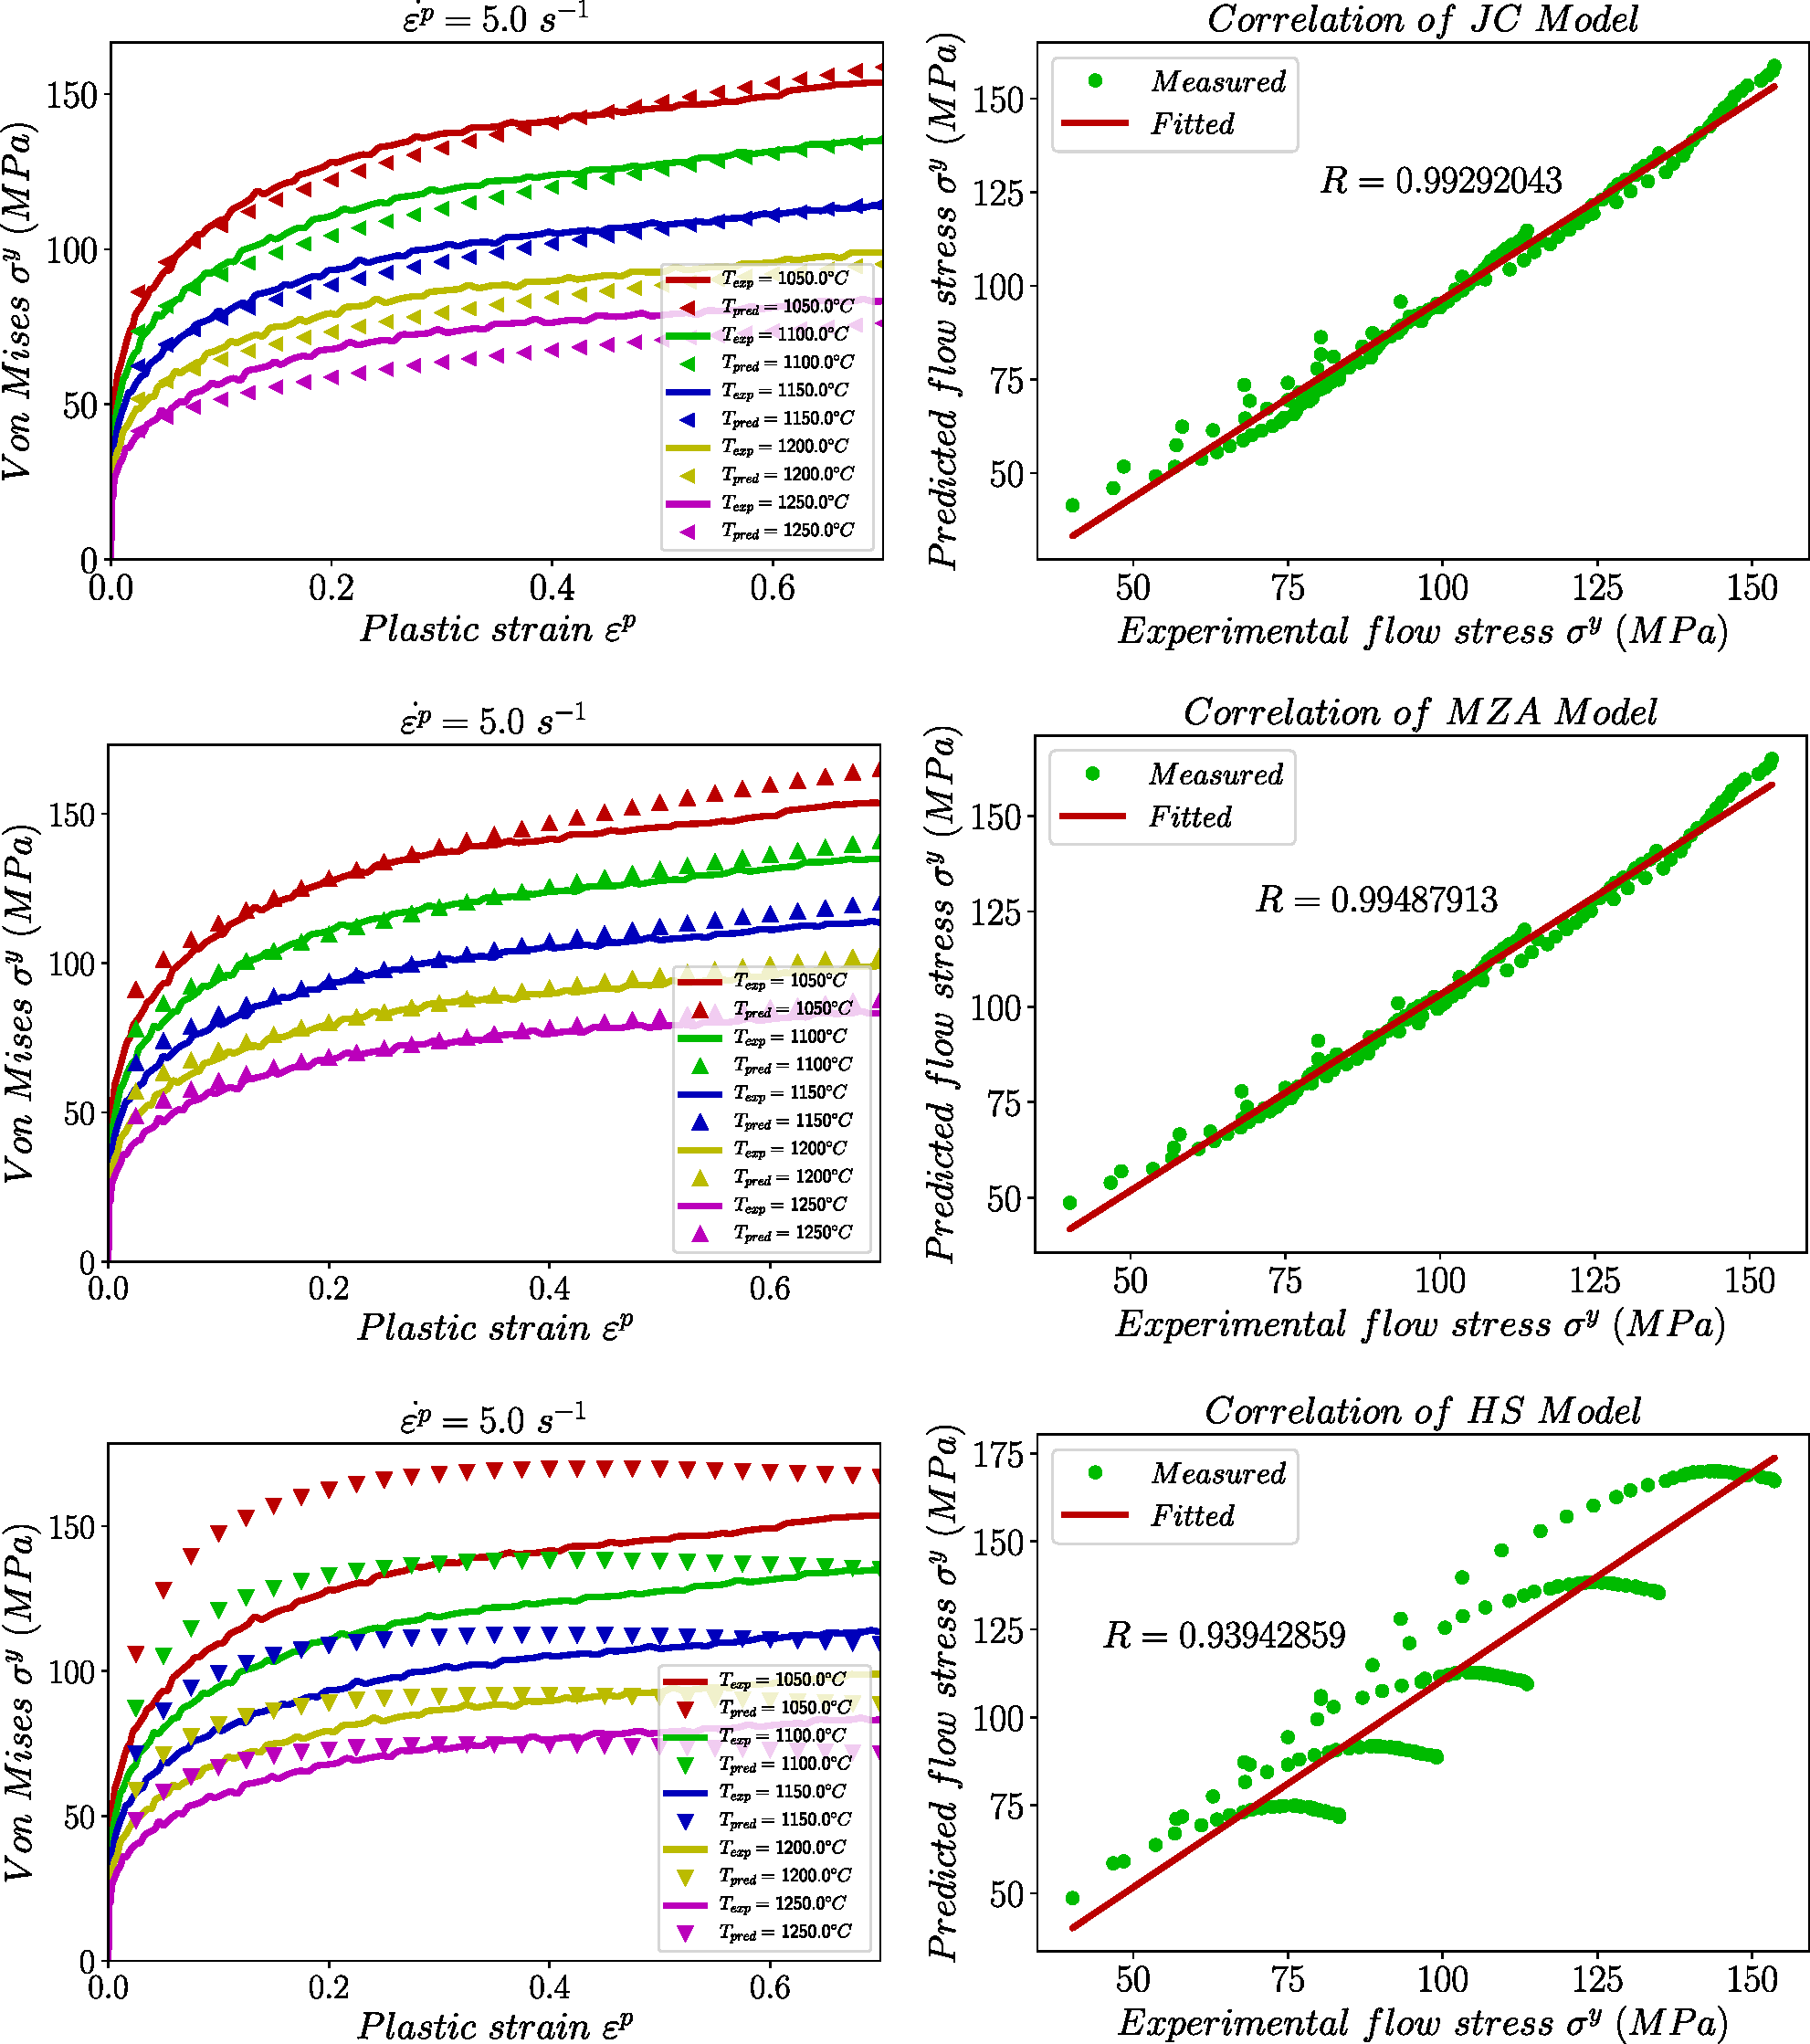
\includegraphics[width=0.98\columnwidth]
{newFigures/exCombinaison1}
\caption{Comparison between the experimental and predicted flow stresses by ANN model for extrapolation estimation}
\label{fig:exCombinaison1}
\end{figure}
\begin{figure}[!ht]
\centering
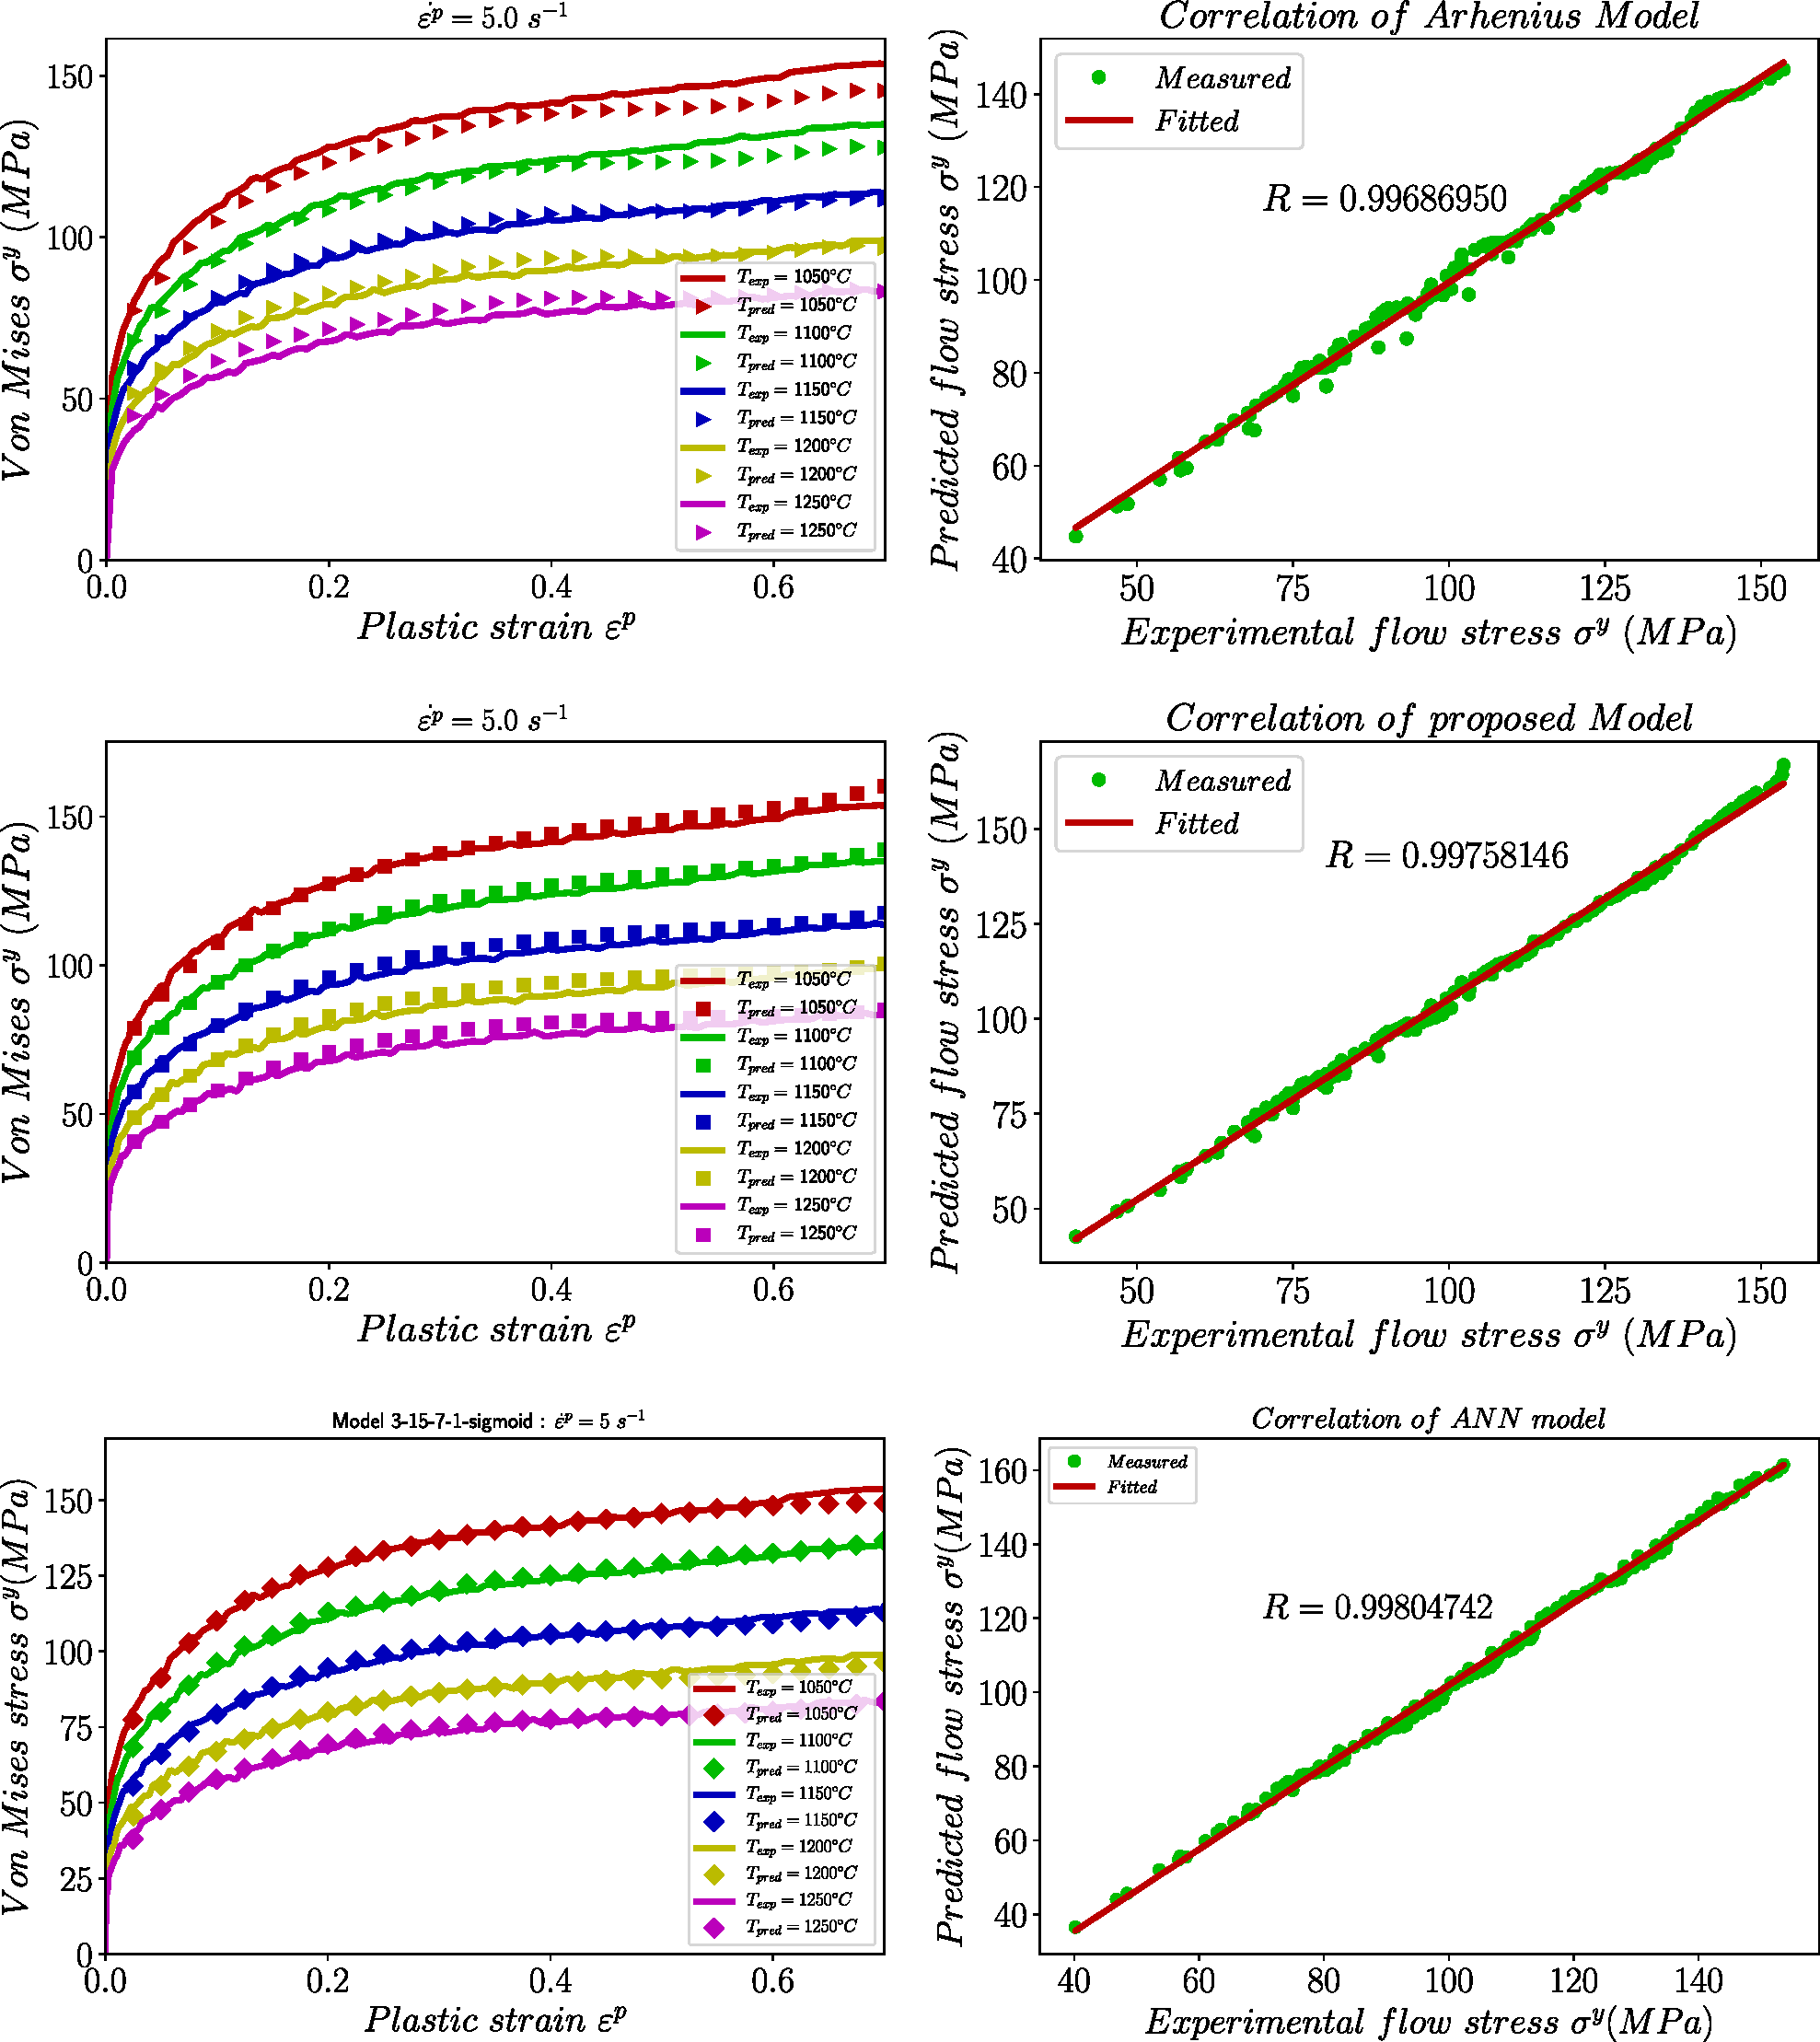
\includegraphics[width=1.02\columnwidth]
{newFigures/exCombinaison2}
\caption{Comparison between the experimental and predicted flow stresses by ANN model for extrapolation estimation}
\label{fig:exCombinaison2}
\end{figure}
\FloatBarrier

%---------------------------------------------------------------------
\section{Conclusion \label{sec:Conclusion}}
In order to describe the high temperature flow behaviour of the modified carbon alloy AISI P20, a comparative study between the phenomenologicalc(JC, MZA, HS, Arhenius and proposed) and ANN models was carried out. This study is done for temperatures ($1050$ -$1250^\circ$C ) and strain rates ($0.001 - 5.0\ \text{s}^{-1}$). Two fundamental works were compared in this study: on the one hand the flow stress prediction capacity of the studied models and on the other hand using these results to predict an interpolation test and another extrapolation test, all validated by experimental data. As a result of this study, the following conclusions were reached:
\begin{itemize}
\item The flow stress increases with strain rate and decreases with the temperature, and strain has significant influence on the flow stress. Analytical models including JC, MZA, HS, Arhenius, proposed and ANN models were developed and a comparison of their predictions was made. Based on the prediction of those phenomenological models, JC and MZA models are not suitable for the AISI P20 alloy because their $\AARE$ are $12.64\%$ and $12.79\%$ respectively. But the Arhenius and proposed models can be used to describe the flow behabiour of this alloy because they have reduced $\AARE$ which are $3.78\%$ and $3.96\%$ respectively. For the ANN model, this coefficient is $0.62\%$. Regarding these results, the ANN model remains the best in terms of predicting the hot flow behaviour of the AISI P20 alloy to which can be added the Arhenius model and the proposed one.
\item All models developed have been validated on interpolation and extrapolation tests. Based on these results, all models have a good prediction of the interpolation although the prediction of the ANN model remains the best. On the other hand, the analytical models do not have a good prediction of extrapolation compared to the ANN model. All these results are summarised in Table \ref{tab:CoefInEx}. 
\end{itemize}

% \bibitem{}
\bibliographystyle{elsarticle-num}
\bibliography{Bibliography}
%\end{thebibliography}
\end{document}
\endinput

